%%
%% This is file `sample-manuscript.tex',
%% generated with the docstrip utility.
%%
%% The original source files were:
%%
%% samples.dtx  (with options: `manuscript')
%% 
%% IMPORTANT NOTICE:
%% 
%% For the copyright see the source file.
%% 
%% Any modified versions of this file must be renamed
%% with new filenames distinct from sample-manuscript.tex.
%% 
%% For distribution of the original source see the terms
%% for copying and modification in the file samples.dtx.
%% 
%% This generated file may be distributed as long as the
%% original source files, as listed above, are part of the
%% same distribution. (The sources need not necessarily be
%% in the same archive or directory.)
%%
%% The first command in your LaTeX source must be the \documentclass command.
%%%% Small single column format, used for CIE, CSUR, DTRAP, JACM, JDIQ, JEA, JERIC, JETC, PACMCGIT, TAAS, TACCESS, TACO, TALG, TALLIP (formerly TALIP), TCPS, TDSCI, TEAC, TECS, TELO, THRI, TIIS, TIOT, TISSEC, TIST, TKDD, TMIS, TOCE, TOCHI, TOCL, TOCS, TOCT, TODAES, TODS, TOIS, TOIT, TOMACS, TOMM (formerly TOMCCAP), TOMPECS, TOMS, TOPC, TOPLAS, TOPS, TOS, TOSEM, TOSN, TQC, TRETS, TSAS, TSC, TSLP, TWEB.
% \documentclass[acmsmall]{acmart}

%%%% Large single column format, used for IMWUT, JOCCH, PACMPL, POMACS, TAP, PACMHCI
% \documentclass[acmlarge,screen]{acmart}

%%%% Large double column format, used for TOG
% \documentclass[acmtog, authorversion]{acmart}

\def\instructions{\instructions}
\def\instructions{\textcolor{red}}

%%%% Generic manuscript mode, required for submission
%%%% and peer review
%\documentclass[manuscript,screen,review]{acmart}
%\documentclass[acmlarge,screen]{acmart}
\documentclass[acmsmall,screen,authorversion,nonacm]{acmart}

\usepackage[dvipsnames]{xcolor}
\usepackage{graphicx}
\usepackage{float}
\usepackage{enumitem}
\usepackage{makecell}
\renewcommand{\cellalign}{tc}
\renewcommand{\theadalign}{tc}
\usepackage{longtable}

%% Fonts used in the template cannot be substituted; margin 
%% adjustments are not allowed.
%%
%% \BibTeX command to typeset BibTeX logo in the docs
\AtBeginDocument{%
  \providecommand\BibTeX{{%
    \normalfont B\kern-0.5em{\scshape i\kern-0.25em b}\kern-0.8em\TeX}}}

\newcommand{\TODO}[1]{\textsf{\textbf{\textcolor{blue}{[#1]}}}}
\newcommand{\QUOTE}[1]{\textsf{\textit{\textcolor{black}{``#1''}}}}

\usepackage{soul}
%% Rights management information.  This information is sent to you
%% when you complete the rights form.  These commands have SAMPLE
%% values in them; it is your responsibility as an author to replace
%% the commands and values with those provided to you when you
%% complete the rights form.
\setcopyright{none}
\copyrightyear{2022}
\acmYear{2022}

%% These commands are for a PROCEEDINGS abstract or paper.
\acmConference[EECS 593 - HCI - FA 2022]{EECS 593: Human-Computer Interaction (HCI)}{August 30--December 15, 2022}{Ann Arbor, MI}
\acmBooktitle{EECS 593: Human-Computer Interaction (HCI), Fall 2022, August 30--December 15, 2022, Ann Arbor, MI}
\acmPrice{00.00}
%\acmISBN{978-1-4503-XXXX-X/18/06}


%%
%% Submission ID.
%% Use this when submitting an article to a sponsored event. You'll
%% receive a unique submission ID from the organizers
%% of the event, and this ID should be used as the parameter to this command.
%%\acmSubmissionID{123-A56-BU3}

%%
%% The majority of ACM publications use numbered citations and
%% references.  The command \citestyle{authoryear} switches to the
%% "author year" style.
%%
%% If you are preparing content for an event
%% sponsored by ACM SIGGRAPH, you must use the "author year" style of
%% citations and references.
%% Uncommenting
%% the next command will enable that style.
%%\citestyle{acmauthoryear}

%%
%% end of the preamble, start of the body of the document source.
\begin{document}

%%
%% The "title" command has an optional parameter,
%% allowing the author to define a "short title" to be used in page headers.
\title{An Exploration of Miscommunciation Intervention in Text Entry}

%%
%% The "author" command and its associated commands are used to define
%% the authors and their affiliations.
%% Of note is the shared affiliation of the first two authors, and the
%% "authornote" and "authornotemark" commands
%% used to denote shared contribution to the research.
\author{Gregory Croisdale}
\authornote{All authors contributed equally to this research.}
\email{gregtc@umich.edu}
\author{Brent George}
\authornotemark[1]
\email{bdgeorge@umich.edu}
\author{Ruei-Che Chang}
\authornotemark[1]
\email{rueiche@umich.edu}
\author{Daniel Chechelnitsky}
\authornotemark[1]
\email{dcheche@umich.edu}
\author{Zhenning Yang}
\authornotemark[1]
\email{znyang@umich.edu}
\affiliation{%
  \institution{University of Michigan}
  \city{Ann Arbor}
  \state{Michigan}
  \country{USA}
  \postcode{48109}
}

%%
%% By default, the full list of authors will be used in the page
%% headers. Often, this list is too long, and will overlap
%% other information printed in the page headers. This command allows
%% the author to define a more concise list
%% of authors' names for this purpose.
\renewcommand{\shortauthors}{G. Croisdale, B. George, R. Chang, D. Chechelnitsky, and Z. Yang}

%%
%% The abstract is a short summary of the work to be presented in the
%% article.
\begin{abstract}
  % Summary of your project goes here. You will update it for each assignment to reflect the new work that you have done.
  % Does abstract properly summarizes whole assignment using the promise, obstacles, solution, and takeaways format in NO more than 250 words.
  %\instructions{Your abstract goes here. Summarize your current state of the project in broadly understandable terms, without use of citations. Word limit: 250 words.}
The communication of emotion is an important aspect of societal interaction. Digital messaging with more accurate emotional communication can make our worldwide connectivity more authentic and less prone to misunderstandings. Textual communication places limitations on implicit messaging, like tone and body language, when compared with face-to-face
interaction. Software interventions in commonly used technologies have the capability to ease these limitations and reduce misunderstandings when using textual communication mediums. Current literature does not extensively explore the nuances of misunderstandings in digital contexts as it relates to
sentimental and grammatical concerns. This paper presents a survey about communication over usable technology to explore this question. The survey results demonstrate the potential impact of a tool which uses sentiment
analysis in non-professional context, and the lack of current tools to address this concern. A contextual inquiry of digital messaging then gives birth to a set of user requirements for a new sentiment analysis tool for
non-professional contexts. Following the isolation of these user requirements and the creation of personas to represent them, prototyping and evaluation showed issues with conforming to existing standards, and this was incorporated into a final prototype designed with Figma. This final prototype was tested to determine user satisfaction, using iMessage as a baseline interface. The test results are statistically significant and demonstrate that users feel the final prototype assists them the emotional context of their non-professional digital conversations. Future digital conversation platforms can use this work to design more user-centered features around the emotional context of message threads.
  
  %Existing solutions emphasize grammatical and syntactical interventions and are more widely adopted in professional contexts.
\end{abstract}

%%
%% The code below is generated by the tool at http://dl.acm.org/ccs.cfm.
%% Please copy and paste the code instead of the example below.
%%
\begin{CCSXML}
<ccs2012>
   <concept>
       <concept_id>10003120.10003121.10003128</concept_id>
       <concept_desc>Human-centered computing~Interaction techniques</concept_desc>
       <concept_significance>500</concept_significance>
       </concept>
 </ccs2012>
\end{CCSXML}

\ccsdesc[500]{Human-centered computing~Interaction techniques}

%%
%% Keywords. The author(s) should pick words that accurately describe
%% the work being presented. Separate the keywords with commas.
\keywords{mobile text entry, sentiment analysis, digital miscommunication}

%% A "teaser" image appears between the author and affiliation
%% information and the body of the document, and typically spans the
%% page.
% \begin{teaserfigure}
%   \includegraphics[width=\textwidth]{sampleteaser}
%   \caption{Seattle Mariners at Spring Training, 2010.}
%   \Description{Enjoying the baseball game from the third-base
%   seats. Ichiro Suzuki preparing to bat.}
%   \label{fig:teaser}
% \end{teaserfigure}

%%
%% This command processes the author and affiliation and title
%% information and builds the first part of the formatted document.
\maketitle

\section{Introduction}
% Does introduction provide proper extended summary of the assignment using the promise, obstacles, solution, and takeaways format with proper citations where necessary. Note that this is a longer summary than the abstract. There is no word limit.

Face-to-face communication between people may be divided into three forms of communication: verbal, vocal, and facial, with the actual verbal content conveying only 7\% of the intended message \cite{in_person_comm_breakdown}. Purely textual communication is now ubiquitous in the digital age. Text, email, social media, and other mediums are used for one-on-one and group conversations. These mediums are purely verbal and cannot utilize vocal or facial messaging to convey the user's full intended meaning. Implicit messaging, like tone and body language, is limited when compared with face-to-face interaction. This can lead to misunderstandings between parties during textual communication that may not have occurred in a face-to-face interaction \cite{Kelly_Miller-Ott_2018}. 

Current literature has not fully explored the causes of misunderstandings across various devices and contexts. These causes may include, but are not limited to, concerns regarding clarity, concision, tone, syntax or grammar \cite{Kelly_Miller-Ott_2018}. Existing solutions focus on syntax and grammar issues in professional settings, on platforms like Microsoft Word and browsers \cite{shin_kim_2022}, while neglecting platforms in non-professional settings, like messaging apps. This paper presents a survey and contextual inquiry to explore this question. 

In this preliminary text-entry survey (n=50), our results demonstrate that participants widely value the use of appropriate tone, specifically in non-professional contexts. This is paired with the participant's view that existing auto-correct solutions overwhelmingly focus on syntactical and grammatical errors, a view supported by current research \cite{Shah_de_2020}, while not providing enough guidance on tone correction. The participants also indicated that misunderstandings are not always the result of mistypings or syntax and grammar issues. Existing auto-correct solutions may not be adequately addressing misunderstandings in these situations. 

In a face-to-face conversation, the intended tone is often communicated through vocal and facial means \cite{in_person_comm_breakdown}. Any imprecision in tone in a purely verbal context, such as textual communication, may have an out-sized effect on any potential misunderstandings. We propose the creation of a project which aims to reduce miscommunication through the provision of feedback and suggestions regarding appropriate tone in non-professional contexts.

Subsequently, we conducted a contextual inquiry to better understand the context of use for a prospective tool. Across various situations, breakdowns were focused on two key events: when an incoming message was first read, and when a drafted message was finished and considered before sending. This led to our formation of user requirements for a tool that would provide support during these key moments to avoid misunderstandings. The full results are listed in Appendix \ref{appendix:contextual_inquiry}.

Following the isolation of user requirements as part of the contextual inquiry as seen in Table \ref{tab:user_requirement}, 5 storyboards and sketch prototypes were generated and critiqued. These critiques were consolidated to a paper prototype, which is depicted by a final persona in a sketch and storyboard that show the context in which the design may be utilized.

Heuristic evaluation and simplified user testing with 5 participants are conducted on this paper prototype design to evaluate it against our user requirements. Table 6 shows the corresponding usability heuristic and severity scores from the heuristic evaluation across all five usability experts. Tables 7-14 show the quality interpretations of the five participants actions and utterances during the think-aloud. 

The key takeaway from this design process is the generation and evaluation of certain features that may be useful in meeting user requirements for a tool that helps users avoid misunderstandings in non-professional digital conversations. Helpful features include color coding words within a given message, and embedding emojis directly in the platform in use that summarizes the emotional context of the message. Additionally, implementations for mobile phones have higher priority because of our context of us. Many potential users will use this for text messaging, which is largely done on mobile devices. Future work may focus on the mobile platform.

With this focus on mind, critiques from the first round of evaluation were incorporated into a final design prototype using Figma. Various screens could be navigated that demonstrated a UI with an emotional color wheel, with each color corresponding to an emotion and a highlight color in the message thread. Users could then interact with this color wheel to select memes to attach to the message thread that matches the desired tone. 

This final prototype meets our user requirements more completely than the predominant iMessage platform. We demonstrate this in a final evaluation: Likert scale rankings by users and a statistical analysis comparing users' satisfaction with iMessage and with the final prototype. The results are statistically significant and indicate that our design has desirable features for navigating the emotional context of a message thread. These features may serve as a valuable starting point for incorporating emotion-based features into other digital conversation platforms.

%The introduction does not expand on the existing obstacles from the abstract. Try to improve that. The design part of the solution is not properly described in the introduction.
%Try to organize the solution by giving the context about why each of your solutions (e.g., survey, contextual inquiry, design) were important and what problems they address.

\section{Related Work}
% Does related work provide a proper summary of related work that describes the current understanding of context of use and how it informed the initial focus of this assignment using proper citations.
\begin{figure}
\begin{center}
    %\fbox{
    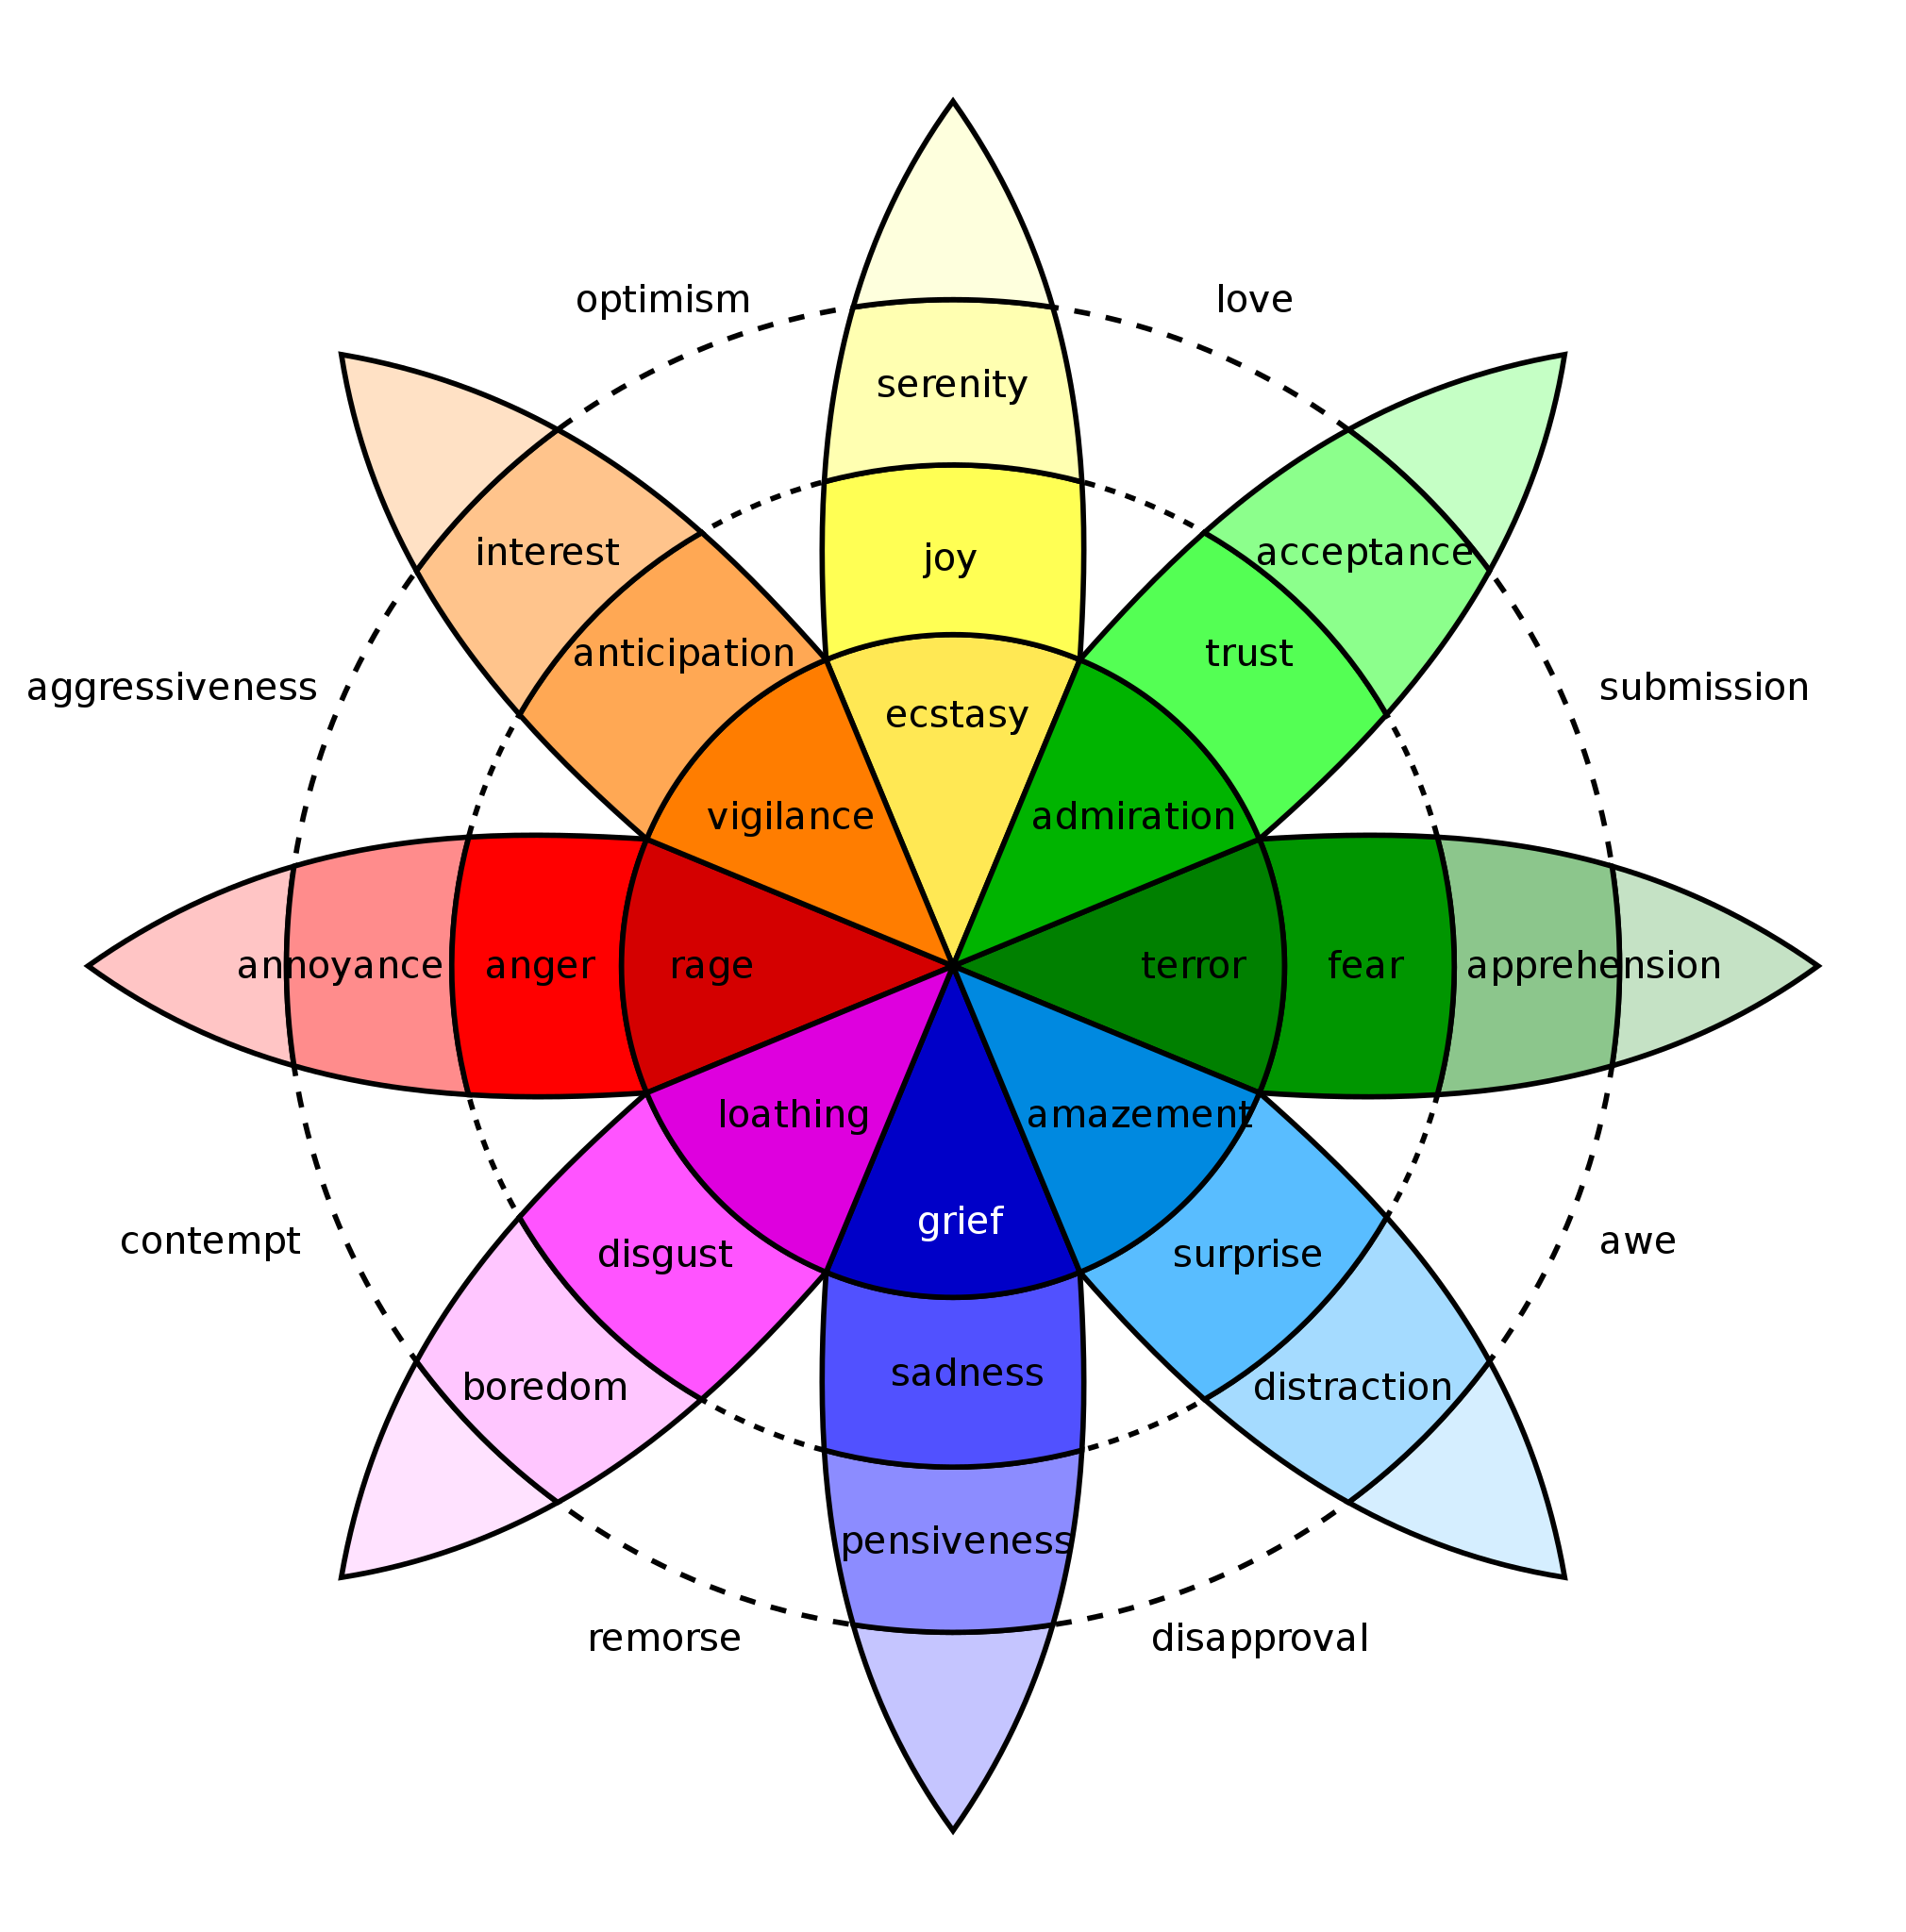
\includegraphics[
        width=0.6\textwidth
    ]{figures/plutchik.png}
    %}
    \caption{Plutchik's Wheel of Emotions}
    \label{fig:plutchik}
\end{center}
\end{figure}
Miscommunications in both personal and professional contexts are exacerbated in textual media such as email and chat \cite{in_person_comm_breakdown}. In personal textual communication, these miscommunications are categorized into the following groups: the interweaving of texting and other activities, a lack of nonverbal cues, use of acronyms and punctuation, and technical features and problems \cite{Kelly_Miller-Ott_2018}. In professional contexts, rather, miscommunications are often caused by information overload and issues which propagate through personalization of a message \cite{jackson2012understanding}.

There is substantial work, both academic and industrial, in the field of correction in text entry, particularly autocorrect. Historically, autocorrect implemented simple fuzzy dictionary lookups with spelling corrections. As advances in NLP allowed for greater machine understanding of text, many systems began implementing context-aware spelling and occasionally grammatical suggestions \cite{Shah_de_2020}, with modern autocorrects often using prediction features. However, beyond the relatively simple correction of spelling or grammar mistakes, correction systems leave much to be desired. Even with a sophisticated autocorrect system, users display an aversion to mispellings which, regardless of the autocorrect system, places a rigid limit on typing speed \cite{Banovic_Sethapakdi_Hari_Dey_Mankoff_2019}.

Digital communication is ultimately focused on the human parties, not on the digital medium. Current autocorrect tools vary in their sensitivity to this fact. Many autocorrect systems focus purely on the language model itself, such as ensuring proper English grammar \cite{shin_kim_2022}. Few systems go beyond language models by acknowledging the emotional contexts surrounding digital conversations. On the other end of the spectrum, tools exist that tap into brain-wave patterns of participants to more accurately express the true intent of the participants \cite{brain_activity_autocorrect}. There is currently a hole in between these two extremes, where a need exists for a correction or suggestion tool with sentiment awareness that doesn't require real-time health data.

Recent innovations in NLP present the opportunity for the creation of this kind of a correction or suggestion tool with sentiment awareness. GPT-3, a near state-of-the-art language model, is capable of text classification, generation, and understanding with remarkable style and tone awareness \cite{Brown_2020}. Furthermore, GPT-3 has proven itself successful in the training and application in new environments, as is evident by the success of the GPT-3-based model Codex, which has been trained on a variety of programming languages and is capable of generating coherent code \cite{Chen_Tworek._2021}. This suggests that GPT-3 could be trained to understand and generate text with a particular tone or sentiment, and that this model could be used to create a correction tool with sentiment awareness. A generally more powerful model, Google's PaLM, presents even more potential for sentiment-aware correction, as is evident through its joke explanation and academic reasoning demos \cite{Chowdhery_2022}.

The field of emotion detection through text is a long-standing one. Beginning with context-agnostic keyword counting, the evolution of this field has closely matched those of other NLP methods \cite{kao2009towards}. Subsequent approaches are identified as being corpus-based, drawing from contextually-labelled lexica (such as tweets) \cite{plaza2020emoevent}, rule-based through text preprocessing and statistical analysis \cite{asghar2017lexicon}, and broadly machine learning methods such as naive bayes or support vector machine \cite{hasan2019automatic}. Each of these approaches are grounded in a combination of emotional theories which attempt to numerically encode the emotional content of a message, such as Plutchik’s Wheel of Emotions as seen in Figure \ref{fig:plutchik} \cite{plutchik1980general}.

Finally, while there are already other automatic feedback program solutions like Grammarly, they  are only functionally efficient in a very specific context rather than flexible tools that can be used widely \cite{grammarlyGood}. Since Grammarly focuses on academic writing, specifically prescriptivist language that is trained on Standard Written English, it therefore doesn't include other important elements of language such as slang, sarcasm, regional dialect differences, and more \cite{grammar2}. More work can be done to further describe language use in daily occasions.

\section{Establishing Focus: Initial Survey}
% Does "Establishing Focus: Initial Survey" section contain a proper summary of the survey purpose, method, tasks and procedures, and participants? Does it contain description of the pilot run, pilot results, and how the results informed the final survey.
%\instructions{This is where details about your work from Assignment 1 goes. Make sure to summarize the purpose of the survey here.}

The purpose of this survey is to understand the context of use for text entry. The team wanted to explore how misunderstandings and mistypings/typo in text entries affect communication, and what can be developed to ease this issue. The survey serves as a guide that helps the team to gain a better understanding of the user groups and the current state of text entry, exposing existing issues within some of the most popular text assistant applications and features in order to elicit user requirements. This section consists of 3 sub-sections: method, tasks and procedures, and participants. The method section includes how the initial survey was developed, a description of each pilot run, and how this pilot runs informed the final survey. Detailed initial and final surveys are attached on appendix (\ref{initial_Questionnaire_Design} and \ref{final_Questionnaire_Design}). Tasks and procedures section includes instructions that were given to participants prior and during the survey, and time span. Lastly, demographic information of participants such as gender, education, etc. will be presented anonymously in its corresponding section. 

\subsection{Method}
% \instructions{What did the survey consist, including the protocol and questionnaire? Make sure to include detailed instruments in the appendix.}

Initially, 4 sections were established for the survey. Each was tailored towards a few specific ideas the group came up with, along with the goal of having the results narrow the scope of the final project. Once the initial structure of the survey was established, the group wrote down a questionnaire sketch for each section. Then, each member took the sketch and created a variant of the survey for the initial pilot run (5 initial questionnaire designs are attached on Appendix \ref{initial_Questionnaire_Design}).

The survey consisted of 4 sections as follows:
\begin{enumerate}
    \item \textbf{Misunderstandings}: In this section, the team aims to gain a better understanding of why, when, and how it happens, and what actions people take to deal with or to prevent misunderstandings in the context of common digital formats, ranging from emails, text messages, social media posts and so on. In the final survey, there are 8 questions in the misunderstandings section. 

    \item \textbf{Mistypings / Typos}: Questions in this section centered around the auto-correct feature and how mistypings/typos negatively affect communication efficiency. Auto-correct is a feature that can detect typos, and some can even detect grammatical errors in real-time. It provides a list of suggestions on how the user might want to fix the error. Modern PC and smartphone operating systems like Windows, macOS, and Android often have auto-correct installed by default. The mistypings/typos section contains 7 questions in the final survey. 
    
    \item \textbf{Tools}: In the tools section, a few commonly used typing assistant software were listed. Follow-up questions were designed to poll the participant's experience with these tools, with the goal of deriving user requirements for a future tool from the results. 
    
    \item \textbf{Demographics}: The demographics section aims to categorize participants by gender, age and education. To further understand the context of use for text entry, this section also includes questions about which social media platforms participants use, what technologies they use for text entry, and how frequently they post or send text messages. The final version of the demographics section contains 7 questions and it is marked completely optional. 
\end{enumerate}

The final survey was implemented using Google Forms. Instructions were given in the header of each question indicating whether a multiple choice, Likert scale, select all that apply, or long-form response was expected.

Each member took their survey and piloted it with 1 participant individually, and wrote down detailed notes on participants' responses, and how they informed the final survey. 

\begin{itemize}
    \item \textbf{Pilot Participant \#1} (Survey Variant \#1, Appendix \ref{var1}): This participant indicated that the misunderstanding section should have a better breakdown of questions, potentially adding questions about the frequency, severity, distribution, types of misunderstandings, etc. The team took this advice and designed a more detailed breakdown of the misunderstanding section in the final survey. 
    \item \textbf{Pilot Participant \#2} (Survey Variant \#2, Appendix \ref{var2}): The participant pointed out that some questions and options from the demographics section were ambiguous and biased. For instance, is the question ``How many languages do you speak'' asking how many languages the participant speaks daily or how many languages the participant can speak. The team then took a closer look at the demographics section, adjusted wordings, removed a few questions that are not closely related but might cause confusion, and edited some of the given options. One revision was having more options for gender and education levels. And making sure that the given options are balanced, no force-answering question, and remove biases as much as possible. 
    \item \textbf{Pilot Participant \#3} (Survey Variant \#3, Appendix \ref{var3}): This participant was confused about the descriptions of ``language of keyboard''. Because a language may includes several keyboard layouts. This is very common in Chinese for instance. This should be further clarified. The original tools section was also confusing in that the questions were too general and not targeted to specific software/hardware keyboard's layout and appearance. So the questions in this section were unanswered. %Ruei-Che's pilot
    \item \textbf{Pilot Participant \#4} (Survey Variant \#4, Appendix \ref{var4}): This participant was not a native speaker of English, so their main comment was to make sure the questions are concise and easy to read (use less "big" words for example). Furthermore, they also agreed that some questions in the misunderstandings section seemed to contain bias. Thus, the team made sure to rewrite and reword the questions that the participant noted as ``long and confusing'' while also accounting for biases. % [Daniel's Pilot]
    \item \textbf{Pilot Participant \#5} (Survey Variant \#5, Appendix \ref{var5}): This participant provided direction into the revision of questions to give them concrete grounding. For example, in the question ``What devices do you use?'', the participant noted the ambiguity of ``use''. The question was rephrased as ``Which devices have you used in the past week?''. Further, the participant indicated that demographics sections for surveys targeted at the general public should generally be at the end so as not to dissuade participation. Finally, this participant indicated that users may have longer-form stories they wish to share regarding miscommunication, so optional long answer questions were added to the survey. %[Gregory's Pilot]
\end{itemize}

The pilot run was effective and informative; the team gathered notes and results from these 5 pilot participants and developed the final survey (the complete final survey can be found in Appendix \ref{final_Questionnaire_Design}). The team decided to put the demographics section towards the end of the survey and made it completely optional. Through research, the team found that having demographics up front is not encouraging. The participant loses patience quickly and is more likely to put ``convenient'' answers and even submit an unfinished survey. 

The 4 sections and their focuses reminds unchanged. As the questions were re-evaluated, additional ambiguous, biased, and focus-answering questions were discovered and subsequently revised, along with the ones that were captured by pilot participants. 


\subsection{Tasks and Procedures}
% \instructions{How was consent for participation sought and administered? What did the task entail? Were participants given any prior instructions? What were they? How long did the task take on an average? How did you go about ensuring quality control of tasks?}

There are four main tasks, each of them included several questions as mentioned above. Before proceeding to the questions sections, we provided an informed consent to notify our participants of our purpose of survey, the confidentiality, and whom they can reach out to if there is any question. Participants were also informed their participation was entirely voluntary, meaning there was no further compensation for taking the survey. Moving on to the next section represents their consent to our survey. The survey took about five to ten minutes to complete.




\subsection{Participants}\label{demo_section}
% \instructions{Please provide demographic information of participants: number of participants, by age, by gender, by disability if relevant for the study, by experience with task, location, any other criteria for recruitment, how they were recruited, were they given any incentives, mode of study conducted (virtual or in-person). How did you decide on the number of participants for your study?}

\begin{figure}[h]
\begin{center}
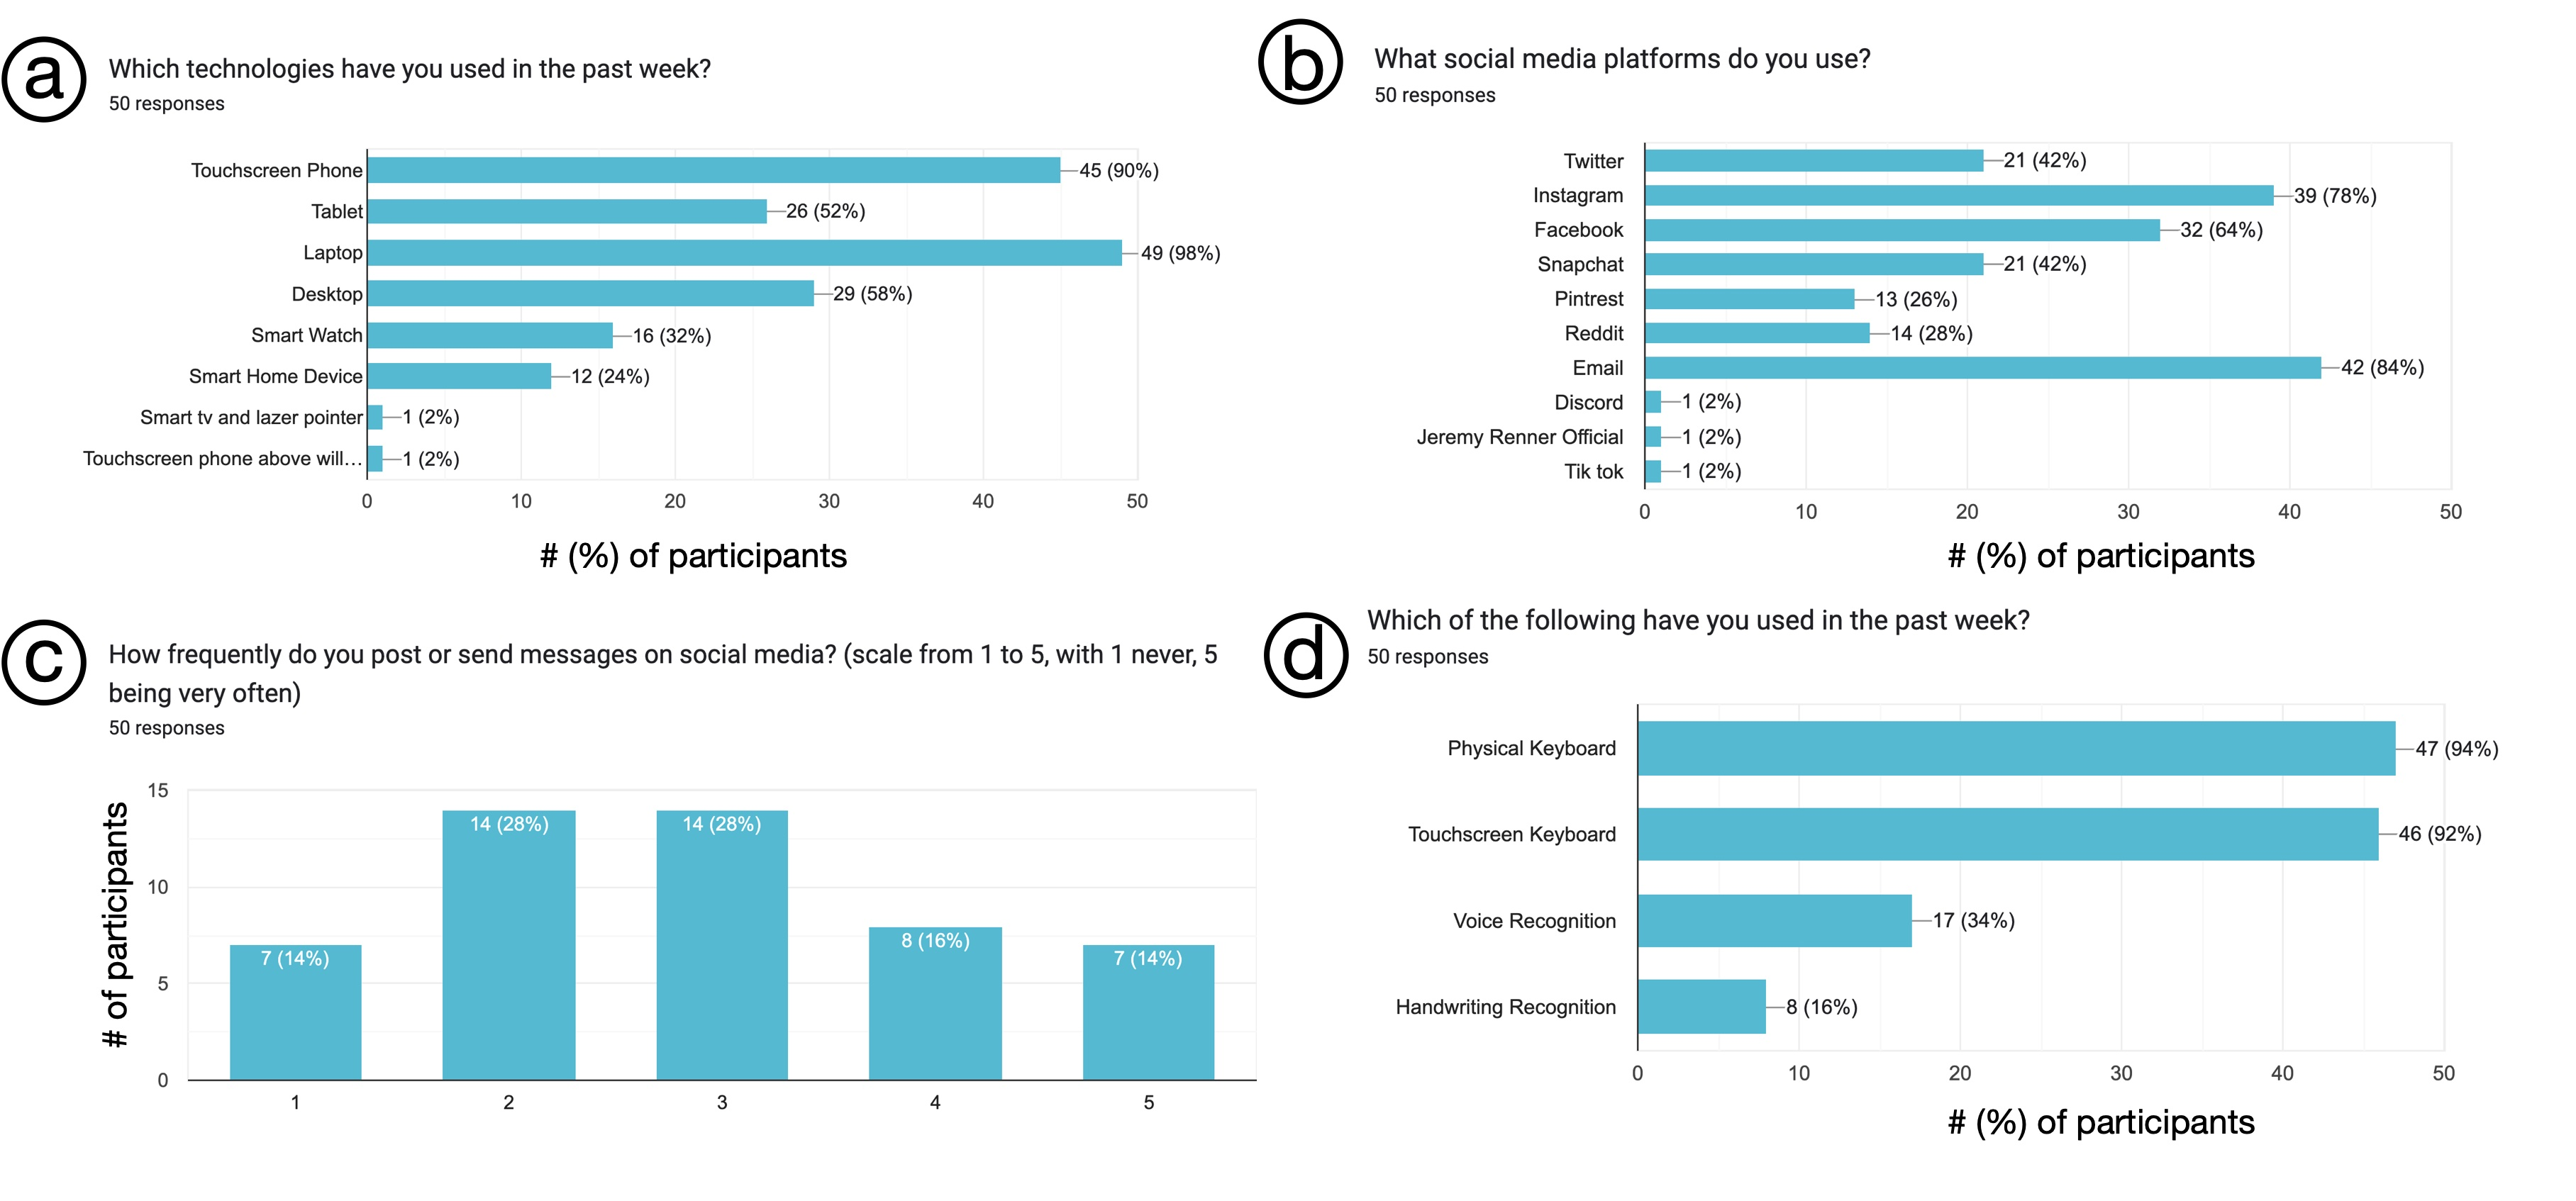
\includegraphics[width=1.0\linewidth]{figures/demographic.jpg}
\vspace{-1.5pc}
\caption{Bar charts for the questions in Demographic section, including the options, number of responses and the percentage of distribution.}
\label{fig:demographic}
\vspace{-1pc}
\Description{}
\end{center}
\end{figure}

Through public posts on social media and word-of-mouth from authors' connections, we received a total of 50 responses in our initial survey. The survey was formatted in Google Forms, and made accessible by internet connection. Thus, participants were not restricted to any location or time to complete our survey. The survey was opened for four days to collect the data. No incentives were offered for completing the survey. 

The distribution of age across our participants is: 4\% (under 18), 62\% (18-24), 22\% (25-34),  2\% (35-44), 8\% (45-54) and 2\% (55-64). 48\% of participants identified as male, 50\% female, and 2\% non-binary. The participant's educational demographics are (from highest to lowest percentage): 44\% (Bachelor's Degree), 34\% (Advanced Degree), 10\% (High School Diploma), 6\% (Some High School), 4\% (Associate's Degree), and 2\% (Certifications from UTK Children's Summer Camp).  

In terms of device usage, 98\% of our participants reported that they used laptop in the past week, 90\% used a touchscreen phone, 58\% used desktop, 52\% used tablet, with several other devices at a significantly smaller percentage (see \autoref{fig:demographic}a for more details). We were also interested in the usage of different forms of text-entry methods. 92\% of our participants used a touchscreen keyboard in the past week, 94\% used a physical keyboard, 34\% used voice recognition and 16\% used handwriting recognition (\autoref{fig:demographic}d). 

To explore miscommunications with text-entry among a broad audience, we were also interested in the communication platforms participants use. Overall, participants used email most frequently (84\%), as well as Instagram (78\%), Facebook (64\%), Twitter (42\%), and other platforms (see more details in \autoref{fig:demographic}b). 

\subsection{Results}

In this section, we present our survey results regarding misunderstandings, mistypings/typos, and tools. 

% Does "Results" subsection in the "Establishing Focus: Initial Survey" section contain a proper summary of survey results including figures containing charts that summarize data using appropriate visualizations.
% \instructions{Please provide detailed results here for each of the questions you asked. Consider combining answers from multiple questions to explore relationships and trends between answers.}





\subsubsection{Misunderstandings}

Tables \ref{tab:difficulty_of_expression}, \ref{tab:damage_misunderstanding}, and \ref{tab:goals_of_comm} summarize the statistical results for the first questions of the misunderstanding section. Figure \ref{fig:misunderstanding} helps further visualize this data.

% In terms of results of question \QUOTE{How difficult is it to express yourself and be understood properly in the following formats (\autoref{fig:misunderstanding}a), on a scale of 1 to 5?}, the average scores reported by the 50 participants were: Text (Mean= 2.6, SD= 1.18), Email (Mean=2.7, SD=1.15), Social Media (Mean=2.74, SD=1.05), Video Chat (Mean=1.84, SD=1.02), and Phone Call (Mean=2.14, SD=1.03). 

\begin{table}[]
\begin{tabular}{|l|l|l|}
 \hline           
             & \textbf{Mean} & \textbf{Standard Deviation} \\ \hline
Text         & 2.6  & 1.18               \\\hline
Email        & 2.7  & 1.15               \\\hline
Social Media & 2.74 & 1.05               \\\hline
Video Chat   & 1.84 & 1.02               \\\hline
Phone Call   & 2.14 & 1.03               \\\hline            
\end{tabular}
\caption{\label{tab:difficulty_of_expression} ``How difficult is it to express yourself and be understood properly in the following formats, on a scale of 1 to 5? (1 is not difficult at all, 5 is very difficult)''}
\end{table}

% For the results of question \QUOTE{How damaging is the average misunderstanding in the following formats, on a scale of 1 to 5?}, the average scores reported by the 50 participants were: Text (Mean= 2.84, SD= 1.11), Email (Mean=3.34, SD=1.11), Social Media (Mean=3.38, SD=1.19), Video Chat (Mean=2.3, SD=0.99), and Phone Call (Mean=2.46, SD=1.07). More detailed distribution can be found in \autoref{fig:misunderstanding}b.

\begin{table}[]
\begin{tabular}{|l|l|l|}
 \hline           
             & \textbf{Mean} & \textbf{Standard Deviation} \\ \hline
Text         & 2.84  & 1.11               \\\hline
Email        & 3.34  & 1.11               \\\hline
Social Media & 3.38 & 1.19               \\\hline
Video Chat   & 2.3 & 0.99               \\\hline
Phone Call   & 2.46 & 1.07               \\\hline            
\end{tabular}
\caption{\label{tab:damage_misunderstanding} ``How damaging is the average misunderstanding in the following formats, on a scale of 1 to 5? (1 is harmless, 5 is very harmful)''}
\end{table}

% For the results of item \QUOTE{Rank the following goals in a non-professional context (for example, communicating with a friend or family member)}, the average scores for each goal reported by the 50 participants were: Clarity (Mean= 2.22, SD= 0.91), Efficiency/Concision (Mean=2.73, SD=1.09), Accuracy (Mean=2.66, SD=0.85), and Tone (Mean=2.4, SD=1.26). More detailed distribution can be found in \autoref{fig:misunderstanding}d. In contrast, to professional context, the average scores for each goal reported by the 50 participants (\autoref{fig:misunderstanding}e) were: Clarity (Mean= 2.2, SD= 1.11), Efficiency/Concision (Mean=2.69, SD=1.06), Accuracy (Mean=2.28, SD=1.11), and Tone (Mean=2.9, SD=1.06). 

\begin{table}[]
\begin{tabular}{|l|l|l|}
 \hline           
\textbf{Non-Professional Context} & \textbf{Mean} & \textbf{Standard Deviation} \\ \hline
Clarity                 & 2.22  & 0.91               \\\hline
Efficiency/Concision    & 2.73  & 1.09               \\\hline
Accuracy                & 2.66  & 0.85               \\\hline
Tone                    & 2.4   & 1.26               \\\hline 
\textbf{Professional Context} & \textbf{Mean} & \textbf{Standard Deviation} \\ \hline
Clarity                 & 2.2  & 1.11               \\\hline
Efficiency/Concision    & 2.69  & 1.06               \\\hline
Accuracy                & 3.28  & 1.11               \\\hline
Tone                    & 2.9   & 1.06             \\\hline            
\end{tabular}
\caption{\label{tab:goals_of_comm} ``Rank the following goals in a professional/non-professional context (1 is most important, 4 is least important)''}
\vspace{-1.5pc}
\end{table}


For the question \QUOTE{What do you do when you are worried about a digital message (text, email, social media post) being misunderstood by the recipient(s)?}, 88\% of our participants would revisit a message in the moment, 72\% would consult another person, 50\% would revisit a message at a later time before sending, 40\% would choose not to send the message, and the 30\% would use a software tool (e.g., Grammarly, etc), indicated in \autoref{fig:misunderstanding}c. 

For the open-ended question \QUOTE{Is there a particular time a message you wrote was misunderstood and there were substantial consequences?}, our participants had diverse situations such as: \QUOTE{Writing an email to the instructor to say that I might be lake for the class this week, but the instructor supposed that I would be late for every class this semester}, or \QUOTE{misplacing a comma I managed to convince a coworker that a project was horribly off schedule and not on schedule.}

Another open-ended question was \QUOTE{Is there a particular time you misunderstood a message and there were substantial consequences?}. Our participants responded \QUOTE{I tend to assume a worse/aggressive tone is intended in text I read than was actually meant, which led to stronger and uncalled for responses}, and \QUOTE{I once spent half a week trying to decipher an email from a coworker who hastily left a “todo” before leaving for vacation.}


\begin{figure*}[h]
\begin{center}
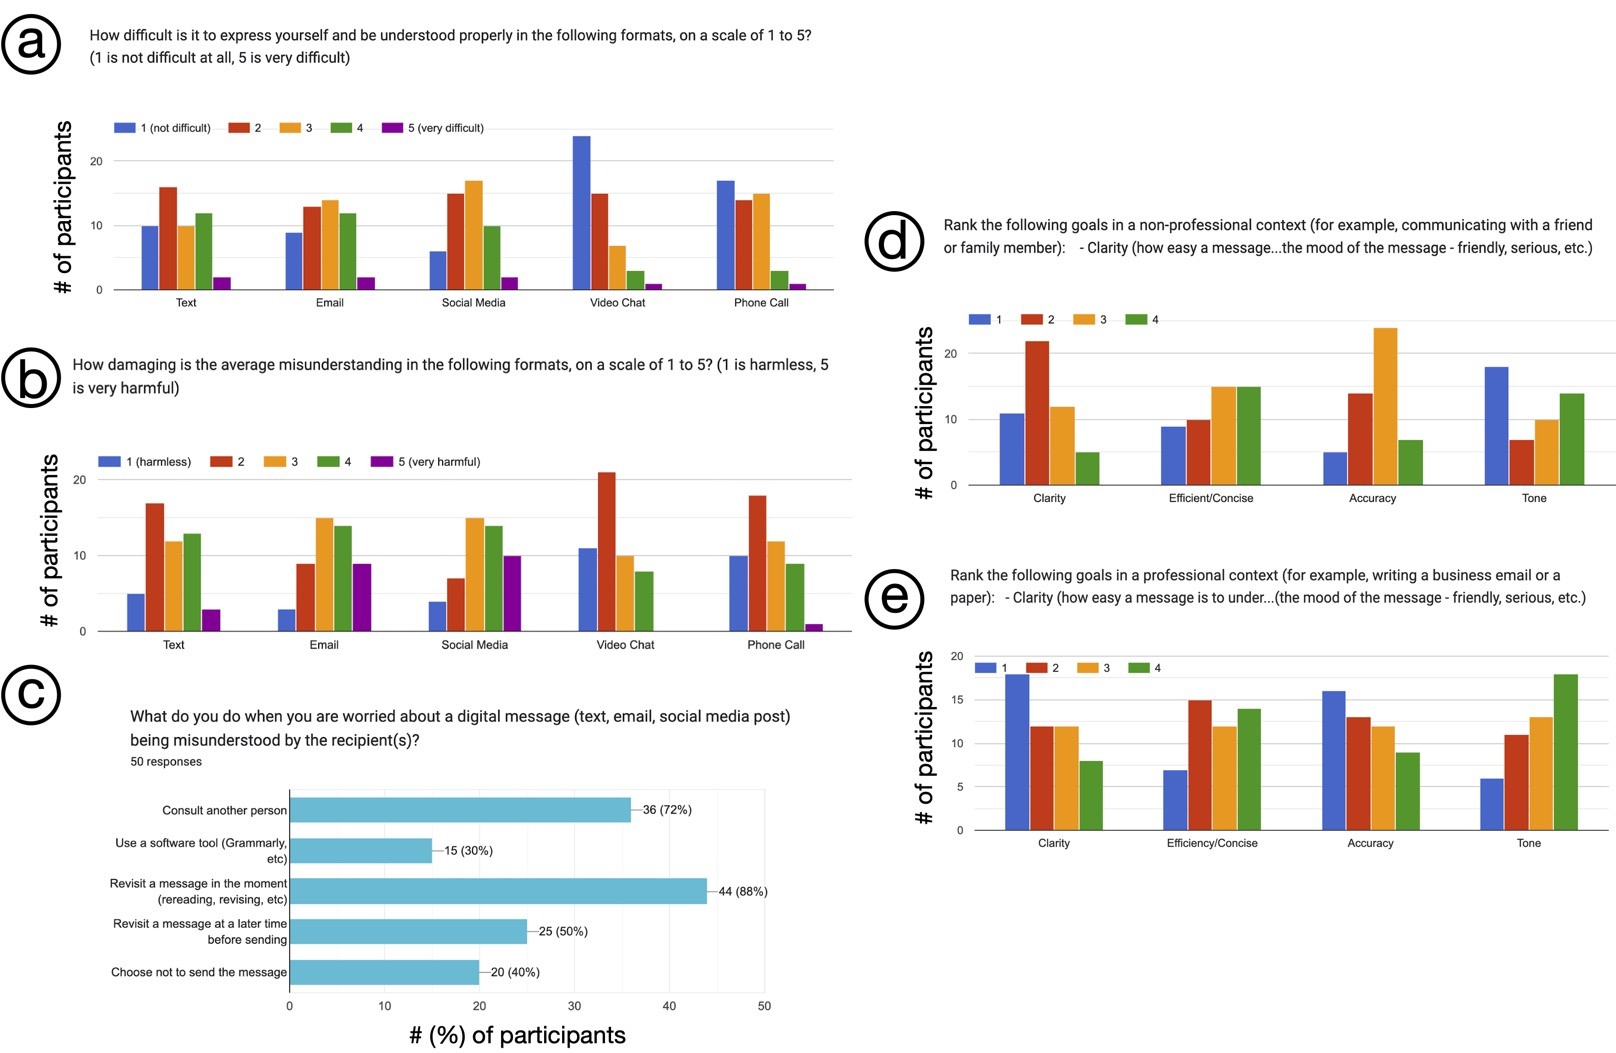
\includegraphics[width=1.0\linewidth]{figures/misunderstanding.jpg}
\vspace{-1.5pc}
\caption{Bar charts for the questions in Misunderstandings section, including the options, number of responses and the percentage of distribution.}
\label{fig:misunderstanding}
\vspace{-1pc}
\Description{}
\end{center}
\end{figure*}



\begin{figure*}[h]
\begin{center}
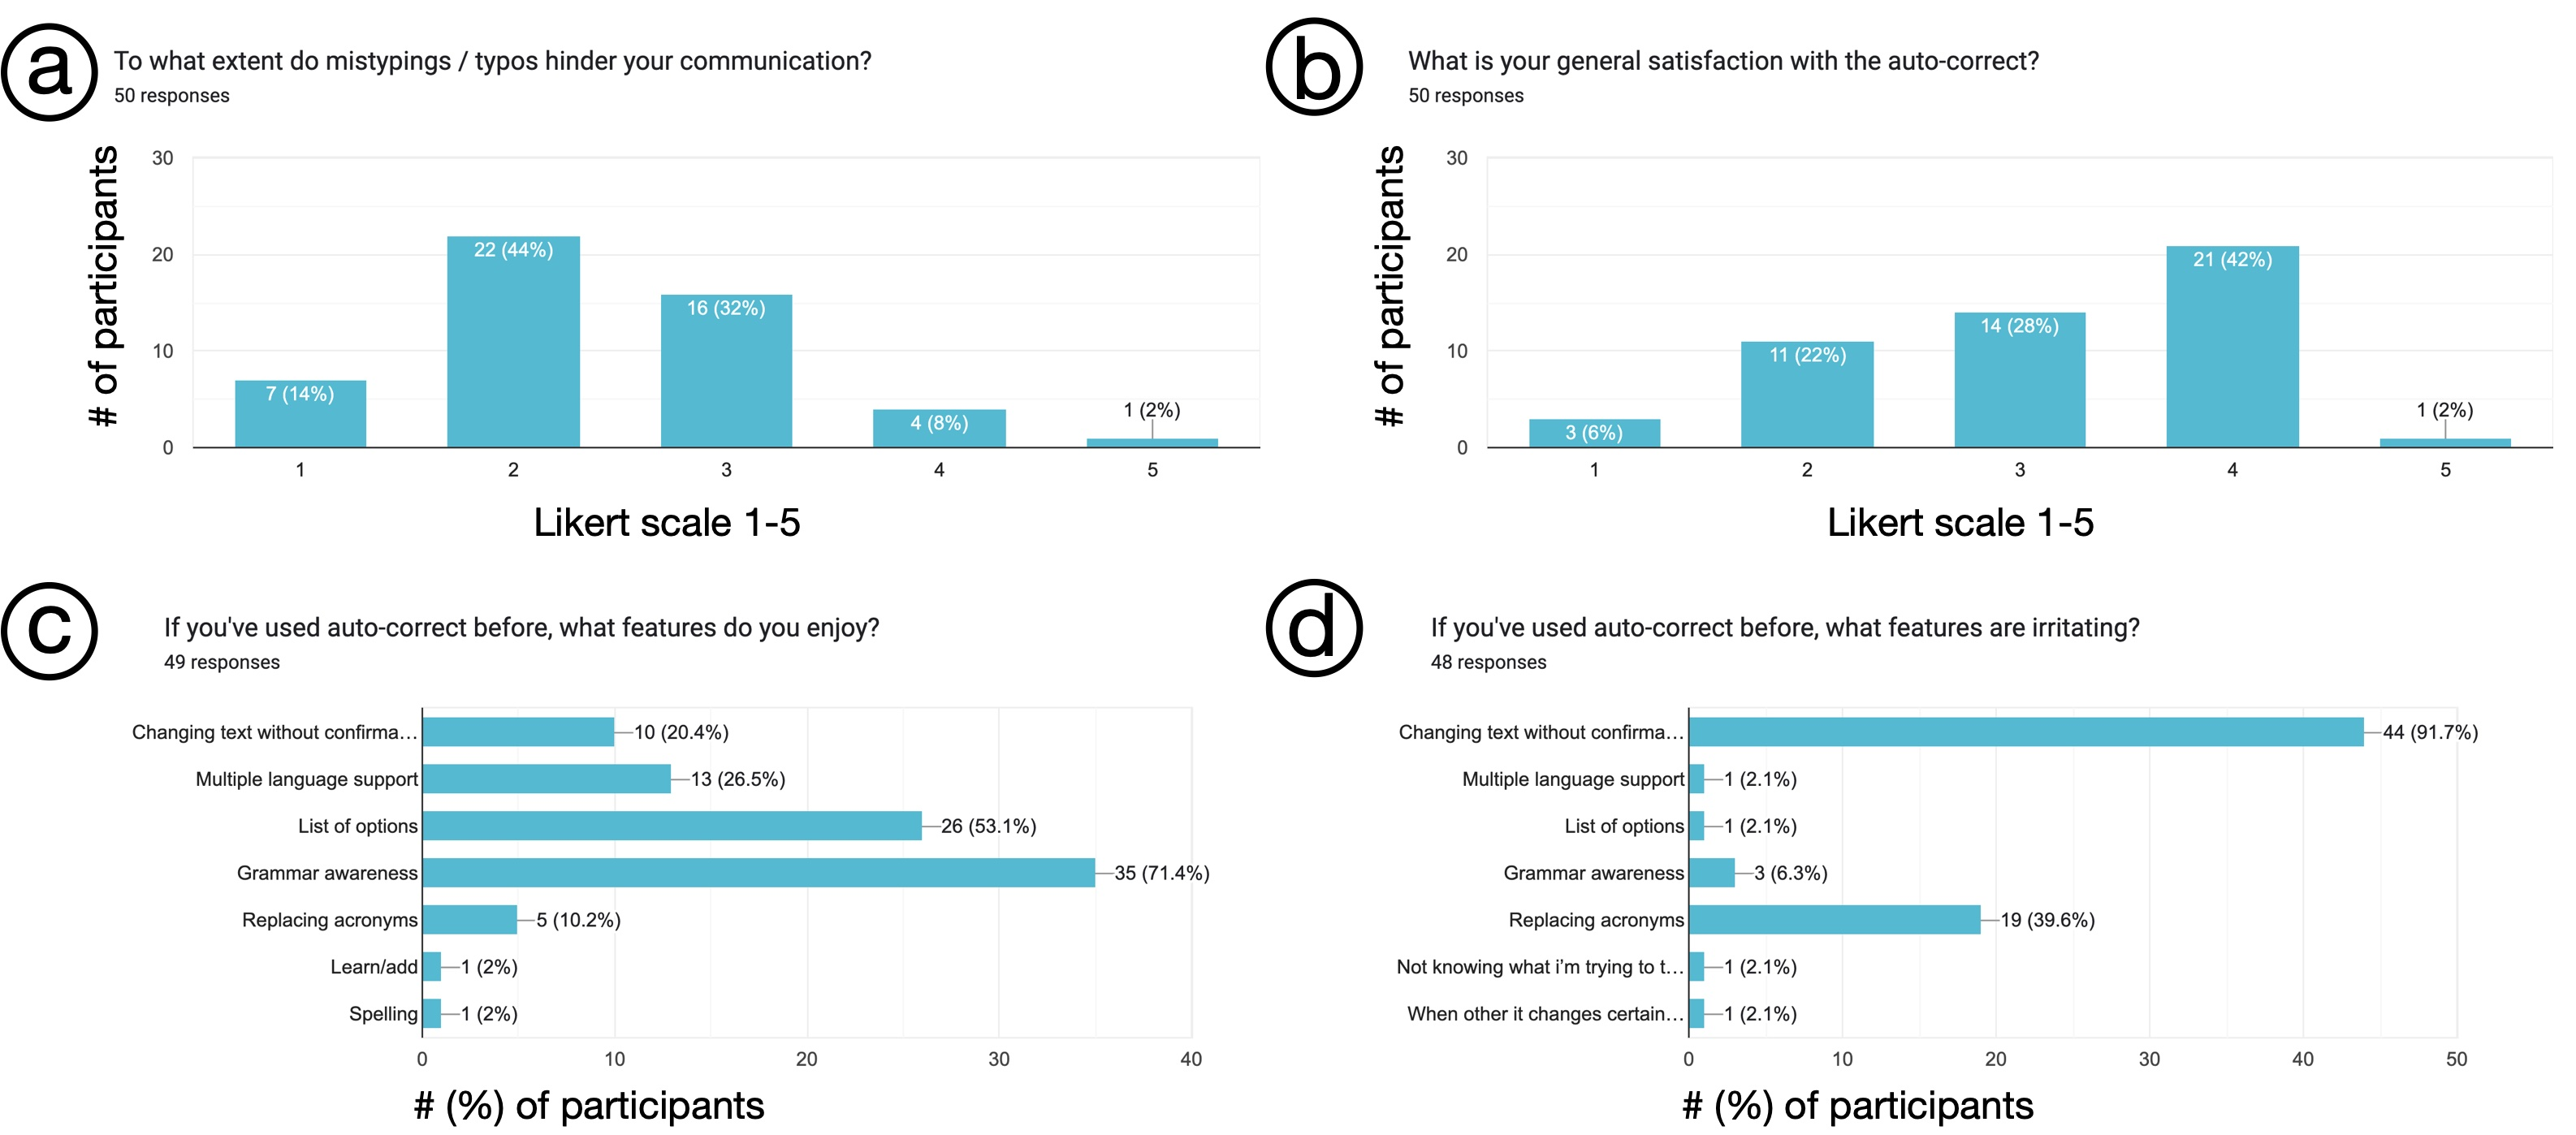
\includegraphics[width=1.0\linewidth]{figures/mistyping.jpg}
\vspace{-1.5pc}
\caption{Bar charts for the questions in Mistypings/typos section, including the options, number of responses and the percentage of distribution.}
\vspace{-1.pc}
\label{fig:mistyping}
\Description{}
\end{center}
\end{figure*}


\subsubsection{Mistypings/Typos}


The first question in this section is \QUOTE{To what extent do mistypings / typos hinder your communication?}. Responses had an average of 2.4 (SD=0.9) under the scale of 1 (not at all) to 5 (extremely). For general satisfaction with auto-correct on a scale of 1 (very dissatisfied) to 5 (extremely satisfied) (\autoref{fig:mistyping} b), participants answered with an average of 3.12 (SD=0.98). Interestingly, 42\% of participants described themselves as satisfied with auto-correct, but only 2\% were extremely satisfied. Also, we found that 45 out of 50 participants regularly use auto-correct while five participants do not (\autoref{fig:mistyping}a). 

As most participants use auto-correct and are generally satisfied, we had varied responses to the question \QUOTE{If you've used auto-correct before, what features do you enjoy?}. 71.4\% of our participants enjoy grammar awareness, 53.1\% enjoy a list of options, 26.5\% enjoy multiple language support, with other choices receiving <=20\% selection rates (\autoref{fig:mistyping} c). 

These results contrast interestingly with the question \QUOTE{If you've used auto-correct before, what features are irritating?}. An overwhelming majority of participants (91.7\%) indicated that ``changing text without confirmation'' is irritating, and some participants (39.6\%) consider ``replacing acronyms'' irritating, with all other answer choices receiving very little support (>7\%) (see \autoref{fig:mistyping}d for more details).

We also had optional open-ended questions, such as \QUOTE{If you had to recommend a feature to an auto-correct system, what would you like to see?} Participants mentioned novel features such as ``context-aware selection'' for the system to switch on/off auto-correct depending on whom they are talking to, or adding a mechanism to allow the user to control the correction instead of being entirely automatic. Another question, \QUOTE{Are there particular situations where you have found yourself mistyping more often than usual? If so, when?}, prompted participants to record various moments they mistyped, including when they are \QUOTE{going fast}, \QUOTE{trying to type out quickly},  \QUOTE{multitasking}, or \QUOTE{[there are] people watching my typing}.   

\begin{figure*}[h]
\begin{center}
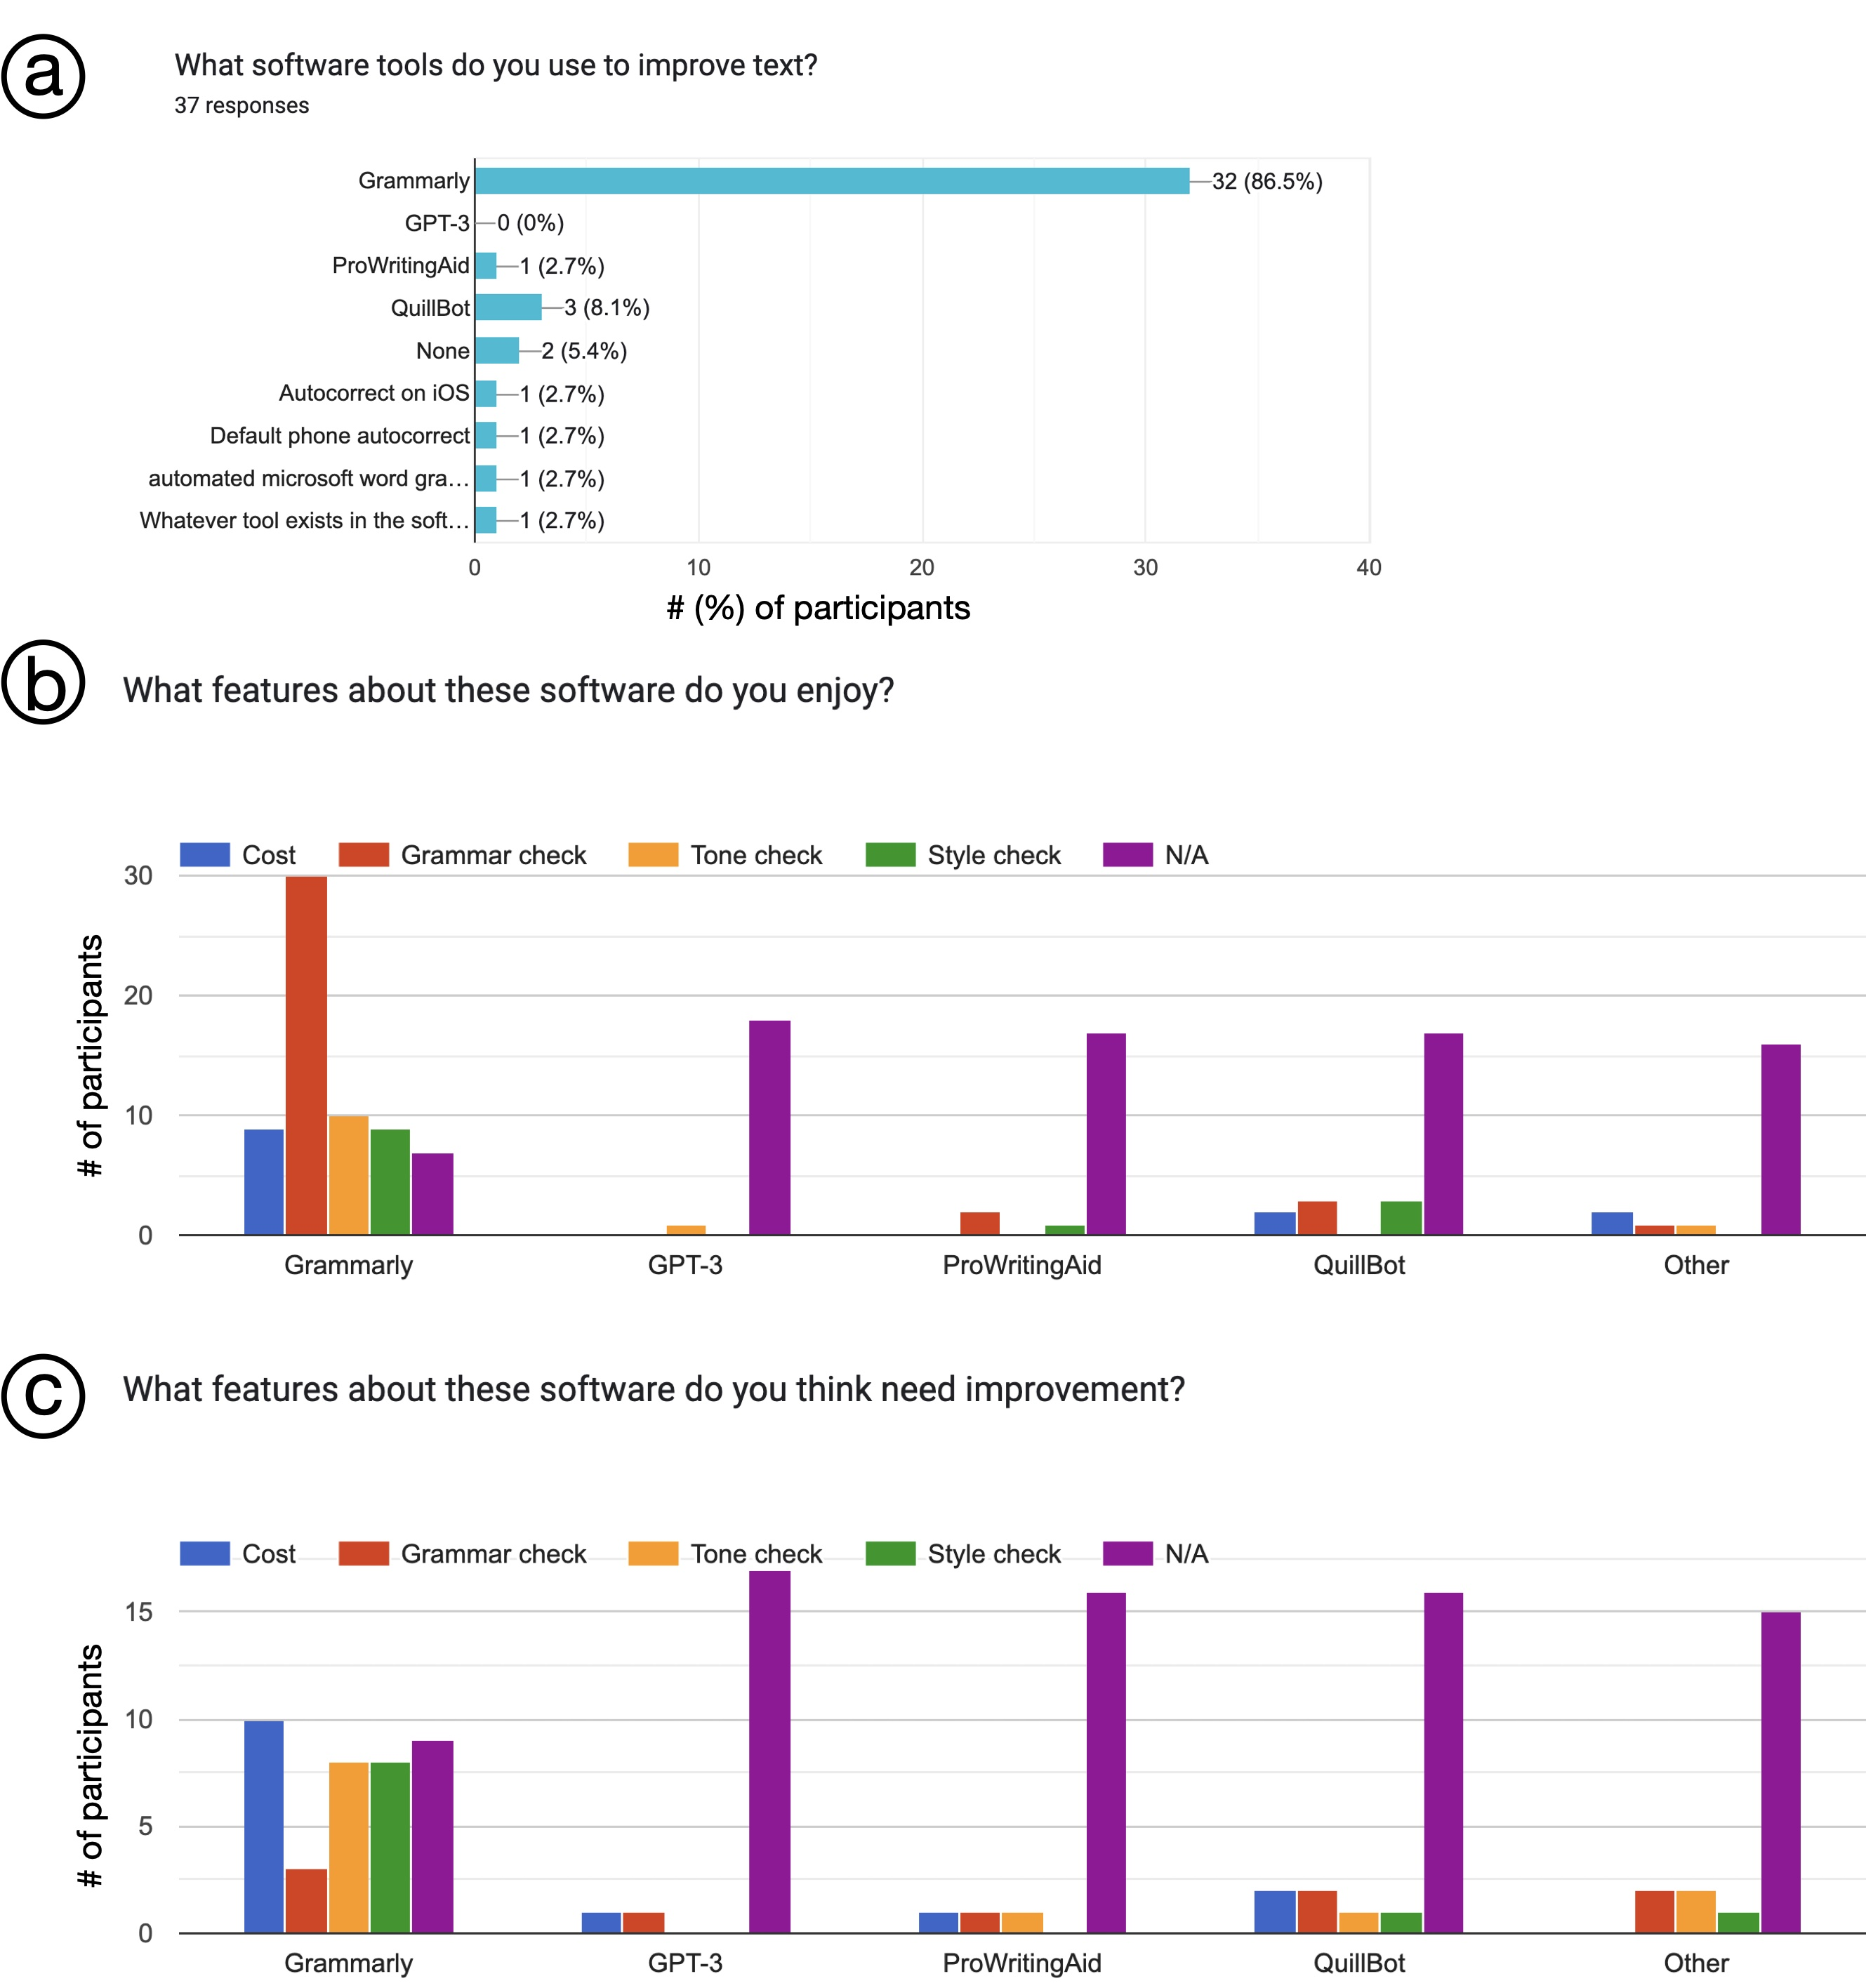
\includegraphics[width=0.7\linewidth]{figures/tools.jpg}
\caption{Bar charts for the questions in Tools section, including the options, number of responses and the percentage of distribution.}
\label{fig:tools}
\Description{}
\end{center}
\end{figure*}


\subsubsection{Tools}
The most popular tool among our participants was Grammarly (86.32\%, \autoref{fig:tools}a). This aligns with the results for the question \QUOTE{What features about these software do you enjoy?}. Participants generally enjoyed grammar check (\autoref{fig:tools}b), which is the primary feature of Grammarly. 

When polled for desired improvements, participants mentioned cost, tone check, and style check (\autoref{fig:tools}c). When asked \QUOTE{How can these tools (for example, Grammarly) be further improved?}, our participants asked for future tools to \QUOTE{predict my next word but not auto-finish}, or \QUOTE{[offer] more customization like with the keyboard short cuts}.

\subsubsection{Demographic information}
The detailed demographic information can be found in section \ref{demo_section}. From the result, we observed that our participants mostly situates in the age of 18-24, which could potentially bias the results due to their higher proficiency in technologies. Also, no participants over 65 years old responded the survey, which could introduce potential bias to the results in that their ways of communication (e.g., tone, words, text, speak, etc) could be different. However, these were what we speculate in the context of current demographic information. 
% More works can be done to understand how the age could potentially affect the results in the context of miscommunication in text-entry.

% For future works or surveys, the range of age should be more evenly assigned and distributed to minimize the potential bias of ages. 


\section{Understanding Context of Use: Contextual Inquiry}

After the initial surveys, our focus was to see how informal writing can be improved using technology.

\subsection{Purpose}
This contextual inquiry is being performed in order to better identify the most impactful project focus, specifically determine user requirements, and determine the platforms and situations in which users would be most to appreciate tonally aware revision assistance.

\subsection{Method}
The project group met beforehand to determine different scenarios to pose to our respective interviewees and which people might be important targets for the interviews. The group developed 10 scenarios, some with specific context including texts. We ordered these scenarios from most important to least important, and agreed to do as many as would fit in a reasonable timeframe (~45 minutes). Through the course of this contextual inquiry, five interviews were performed, each by a different interviewer.

\subsection{Participants}

The 5 participants interviewed can be identified as follows: U01, a 55-64 year old non-native English speaker; U02, a 18-24 year old non-native English speaker; U03, a 25-34 year old non-native English speaker; U04, a 45-54 year old native English speaker; and U05, a <18 year old native English speaker. These participants were selected in order to provide context for a broad range of users.

\subsection{Tasks and Procedures}
The contexts that were explored during the course of this contextual interview were among the following:
\begin{enumerate}
    \item Sending a logistic text
    \item You’re meeting up for lunch with someone soon and you don’t know where
    \item Posting a life update on social media
    \item You’re changing schools and moving away from your city
    \item Sending an emotionally charged text
    \item You want to apologize for something you said earlier
\end{enumerate}

To begin the contextual interview, the context of the research was communicated to the participant followed by the collection of demographic information. After this, participants were presented with a scenario with some individualized context (i.e., you receive a discord message, you see a post on Reddit). Upon being given the scenario, the participant showed the navigation to the application they desired to use and spoke aloud as they approached the scenario, generally on their phone. During their explanation of what their actions and their thoughts, the interviewer asked clarifying questions. Sometimes, the interview would provide potential responses to the interviewee’s messages in order to fully understand the interaction. The interview target length was 45 minutes.

\subsection{Results}
% Does "Results" subsection in the "Understanding Context of Use: Contextual Inquiry" section contain a summary of all Contextual Interviews including a summary of different aspects of the participants' context as specified by consolidated sequence and flow diagrams, and the affinity diagram. Do the results point to specific interpretations and diagrams?

\begin{center}
\begin{table}[h]
\begin{tabular}{|c|c|c|c|}
\hline
\textbf{Participant} & \textbf{Age} & \textbf{Native English Speaker} & \textbf{\#Scenario} \\ \hline
1(DC)                    & 55-64           & No                              & 2                   \\ \hline
2(ZY)                    & 18-24           & No                              & 4                   \\ \hline
3(RC)                    & 25-34           & No                              & 4                   \\ \hline
4(BG)                    & 45-54        & Yes                             & 4                   \\ \hline
5(GC)                    & <18           & Yes                             & 3                   \\ \hline
\end{tabular}
\caption{\label{tab:participant_overview} An overview of participant demographics and the provided number of scenarios. }
\vspace{-1.7pc}
\end{table}
\end{center}

\textbf{Participant \#1}: 2 scenarios were provided to this participant, to explore the context of "Sending a logistic text" and "Posting a political opinion on social media".

\begin{center}
\begin{enumerate}
    \item \textbf{It’s 10 a.m. and you had discussed yesterday over email to meet up with another coworker for lunch later today. You agreed on the time 1 a.m. but you don’t know where this will take place}: The participant opens their laptop, clicks to open Chrome, and then clicks opens Gmail (DC-U01-01-01). If a login is prompted, they put in their login information. The participant then types the name of the person into the “Search in mail” bar and find the prior conversation (DC-U01-01-02). If they cannot find the previous conversation they simply click “Compose” for a new message. If they do find the previous message, they re-read the thread to make sure they don’t see a location or a reference to one. The participant then clicks “Reply”(DC-U01-01-03). If a location was not mentioned, they will write a sentence asking where the location is, and then sign their name. If the location was mentioned, they will write a sentence asking to make sure the location was coffect, and sign their name. If at this time the Google correct feature appears to rephrase, the participant will read aloud the rephrase to make sure to themselves that it sounds good (DC-U01-01-04). If the correction sounds better than what was written before, they accept the correction. Otherwise not (DC-U01-01-05). If the colleague responds in a reasonable time before the meeting, the participant will reply with a short message to acknowledge that the conversation is over (DC-U01-01-06). If the colleague does not respond, and no location is mentioned, the participant will simply ask and follow-up with them later at the weekly in-person staff meeting. Detailed interpretation, sequence, and flow diagrams are attached in Appendix (\ref{C-DC}, \ref{ISeqDiag} and \ref{IFlowDiag}). 
    
    \item \textbf{The Roe v Wade Supreme Court announcement has just come out, and there is a flood of posts already from your friends on Facebook. You are going to make a post as well}: The participant will first open up their laptop, click to open Chrome, and then click to open Facebook (DC-U01-02-01). If a login is prompted, they put in their login information. The participant will then see the other posts and like whichever ones they agree with (DC-U01-02-02). Here, they will also check to see if they have received any Facebook Messenger messages and respond to those if seen. Since these messages are informal and or in a language that does not have auto-correct, they will simply read over the message quickly before sending it (DC-U01-02-03). Next, the participant will click “Make post”. Here, they will insert a relevant article they have found online or a picture, since the post needs to “attract attention” (DC-U01-02-04). Next, they will write their opinion, but also make sure to keep away from “crude” language since my participant likes to consider their public image as a polite person (DC-U01-02-05). They will then ask their partner who has lived in the United States longer to read over the message for them to “get another pair of eyes” on it to make sure it is free from grammar mistakes (DC-U01-02-06). They then might also run it through Grammarly to triple check it is free of any overall thematic errors (DC-U01-02-07). Next, one they post, they will keep checking in to see how many people like/comment (DC-U01-02-08). If many people are upset, they will remove the post, otherwise they will leave it up (DC-U01-02-09). Detailed interpretation, sequence, and flow diagrams are attached in Appendix (\ref{C-DC}, \ref{ISeqDiag} and \ref{IFlowDiag}). 
\end{enumerate}
\end{center}

This participant prefers using the laptop as their main driver for communication, sending logistic texts, and posting on social media. Once the message is fully written down, they read through the text and make sure it is free of errors, and the tone is sound and polite. Some advantages of using laptops are easier to type, and tools provided easy access to tools like Grammarly compare to smartphones. 

\vspace{7pt}

\textbf{Participant \#2}: 4 scenarios were provided to this participant, to explore the context of "sending an emotionally charged text" and "set up a meeting for the first time".

\begin{center}
\begin{enumerate}
    \item \textbf{You want to apologize for something you said earlier}: The participant first took out an android smartphone from the pocket and unlocked it (ZY-U02-1a-01). He uses WhatsApp as a major communication tool. He unlocked the phone and located the WhatsApp icon, then clicked to enter the user interface. Then the participant scrolled through many existing threads and found the old thread with the friend (ZY-U02-1a-04). He simply opened the thread and started typing. He explained that, for the given context, he tends to write a long text, talk about the earlier situation with the friend, and explain why he said what he said, like “he was having a rough day”, etc. If it is his fault, he will admit and apologize in the message. Before sending the long message to the friend, he double-checked the text and made sure there were no grammatical errors, and that the tone was sincere and honest (ZY-U02-1a-06). Once the text is sent, he puts the phone away; because he assumes that the friend might still be mad and may not reply to his message right away. But he checked the phone more frequently than usual, waiting for responses from the friend. Detailed interpretation, sequence, and flow diagrams are attached in Appendix (\ref{C-ZY}, \ref{ISeqDiag} and \ref{IFlowDiag}). 
    
    \item \textbf{You are very nervous about the big presentation tomorrow, you want to text someone close to you for comfort}: The participant mentioned that he doesn’t usually do that. But if he were to perform this task, he will likely use WhatsApp again, since many of his close friends are on WhatsApp (ZY-U02-1b-02). Similar process as above, he entered the interface and located an old thread with a close friend. Then, start typing right away (ZY-U02-1b-05), his general mindset is that he is not trying to start a conversation with this friend, rather he will talk about how he feels about the presentation, and hope to feel better afterward. He also mentioned that it would still be great if the friend replies. But it is okay if that didn’t happen. He will send many short messages in a short period of time, and it is not likely that he is going to double-check the text. Afterward, he put the phone away, since he did not expect a response (ZY-U02-1b-07). Detailed interpretation, sequence, and flow diagrams are attached in Appendix (\ref{C-ZY}, \ref{ISeqDiag} and \ref{IFlowDiag}). 
    
    \item \textbf{Set up a meeting with someone in a different time zone}: The participant prefers using his laptop to send a formal email. He first located his laptop, then started looking for the laptop charger, since the laptop is old and the battery doesn’t last for a long time; he almost always has it plugged in (ZY-U02-2a-01). Then he opened up a browser and navigated to the Gmail page, and created a new email thread. Then he typed a very formal email, including greetings, and a virtual link, date, and time for both time zones (ZY-U02-2a-03). The participant mentioned that he doesn’t use any external text assistance tool like Grammarly, only the built-in spell-checker. He also mentioned, if it is not urgent, he often left the email in the draft and plans to come back later for the final refinement (ZY-U02-2a-05, 06). Since he might have new ideas or new perspectives later on. Once the draft is ready, he sends it to the person and waits for responses. Detailed interpretation, sequence, and flow diagrams are attached in Appendix (\ref{C-ZY}, \ref{ISeqDiag} and \ref{IFlowDiag}). 
    
    \item \textbf{You wanted to set up an informal meeting with someone at a coffee shop}: The participant decided to use his smartphone. As usual, he opened WhatsApp and created a new thread with this person (ZY-U02-2b-02). Even though WhatsApp is connected to phone numbers, the participant still prefers using the app, instead of using phone numbers. He explained that he received many scam messages and he tends to ignore phone messages. Then he typed a casual text asking about what would be a good time and location (ZY-U02-2b-05). Since the participant always plans things ahead of time, he doesn’t expect to hear from the other person right away. So he put the phone away (ZY-U02-2b-06). Detailed interpretation, sequence, and flow diagrams are attached in Appendix (\ref{C-ZY}, \ref{ISeqDiag} and \ref{IFlowDiag}). 
\end{enumerate}
\end{center}

Although participant \#2 is not a native English speaker, he speaks fluent English and is very confident about his writing. In most cases, he does not use any text assistance tool. But when sending long emotionally charged messages with his smartphone, he is more likely to check the tone, and fine-tune the text to prevent misunderstanding. In contrast to participant \#1, this participant noted that software like Grammarly often alters their intents slightly. If it is not urgent, the message will be left in the draft and they come back later to edit. 

\vspace{7pt}

\textbf{Participant \#3}: 4 scenarios were provided to this participant, to explore the context of "Sending a logistic text" and "Posting a life update on social media".

\begin{center}
\begin{enumerate}
    \item \textbf{You’re meeting up for lunch with someone soon, and you don’t know where}: The participant first took her phone out and tried to open WeChat to search the previous chatroom with her friend. The interpretation of choosing WeChat was due to the assumption that her friend will be most likely receive and respond the message in time, as this is their primary communication channel. Searching on the chatroom also helps to minimize the time for searching on the long contact list. However, if the time becomes urgent or her friend still not respond, she would directly have a phone call to her friend to ensure to get the immediate response, as she assumed her friend turned off the notification of WeChat or in situation that cannot observe the message. Detailed interpretation, sequence, and flow diagrams are attached in Appendix (\ref{C-RC}, \ref{ISeqDiag} and \ref{IFlowDiag}). 

    \item \textbf{You’re gonna get interviewed remotely in half-hour but the link to the virtual room is missing}: The participant chose to use her laptop and opened the email app to searched for the previous email thread with the HR. The interpretation of this behavior is that replying the previous thread can help HR to locate and identify her more quickly which can save more time. Aside from looking for the link for meeting, another reason to check the emails is to ensure if she did miss the email and the link, and should be responsible to this mistake. After sweeping out through the emails and finding nothing, she will directly contact HR by all means. At the same time, if she was aware of who would be her interviewers or one should be involved, she would also inquire about and notify them of the missing link. The interpretation behind this is that she wanted to demonstrate her efforts in addressing this problem and hope the other side can understand this situation. Detailed interpretation, sequence, and flow diagrams are attached in Appendix (\ref{C-RC}, \ref{ISeqDiag} and \ref{IFlowDiag}). 

    \item \textbf{You’re moving away from your city and you want to share with friends.}: The participant said she was not a person who are eager to share such private news. But when it comes to a required thing, she would also choose WeChat either as her friends also use it. The workflow is to take pictures on the new decorations of her new house, add location information, add descriptions. The reason to add location is to make people know the rough area she is currently in, like now in Ann Arbor. By doing this, her friends nearby Ann Arbor can also come and maybe she can host a party. Before posting everything, there is an interesting feature in WeChat - they can block some people from seeing the post or they can also notify selected people of this post. The reason to do so is to prevent someone from seeing the post (i.e., teachers, parents, etc). After setting up these all configurations, she will just post it, put away the phone and wait for responses because collecting replies take time. Detailed interpretation, sequence, and flow diagrams are attached in Appendix (\ref{C-RC}, \ref{ISeqDiag} and \ref{IFlowDiag}). 

    \item \textbf{You just get married and want to post your wedding pictures and describe them.}: As wedding is a very private thing to her, she did not want to post on the WeChat, where many acquaintances still are there. However, she also wanted to share her wedding and take this share a diary or alive memory online. She thus chose Xiaohongsu, which is an app that keep all authors anonymous on their posts. Same workflow to post things, she started by selecting photos on her wedding, but this time, she would like to add hashtag \#wedding to increase the visibility on the search engine. By doing so, she expected to get many replies and inquiries from strangers who might also be planning a wedding. Another reason to keep this post anonymous is that she did not want to be criticized by her friends how good or bad her wedding is, and did not want to be compared with others, which makes her stressful. After posting, she will just put the phone away and wait for the responses. Detailed interpretation, sequence, and flow diagrams are attached in Appendix (\ref{C-RC}, \ref{ISeqDiag} and \ref{IFlowDiag}). 
\end{enumerate}
\end{center}


\vspace{7pt}

\textbf{Participant \#4}: 4 scenarios were provided to this participant, to explore the context of "Sending a logistic text", "Posting a life update on social media" and "sending an emotionally charged text".

\begin{center}
\begin{enumerate}
    \item \textbf{User receives a text asking for clarification on existing plans}: The participant clicked on the notification and it opened the app directly (BG-U04-101). Once the participant decided to read the entire message after reading the preview. They opened up the thread, read the entire message, then reply with a simple message like "ok" (BG-U04-105), then put the phone away, and don't expect any responses. Detailed interpretation, sequence, and flow diagrams are attached in Appendix (\ref{C-BG}, \ref{ISeqDiag} and \ref{IFlowDiag}). 
    
    \item \textbf{User recently got married and is going to make a social media post}: The participant first took her phone out, and located Facebook, since this is the only platform she uses (BG-U04-201). And she clicked on create a post and typed out short and straightforward messages like "Just got married!". Then she scrolls through the Photo app and found a single photo she likes that includes her and her spouse (BG-U04-203). And attached it to the Facebook post. Once the post is sent, she will keep track of the comments. Detailed interpretation, sequence, and flow diagrams are attached in Appendix (\ref{C-BG}, \ref{ISeqDiag} and \ref{IFlowDiag}). 
    
    \item \textbf{User had a recent in-person interaction with a friend where they said something that hurt the other person’s feelings. User is going to apologize using a digital medium}: The participant unlocked her smartphone through about how to phrase her apology. And typed out some text describing the situation and explain herself (BG-U04-303). While typing the participant actively checks for error and tone. Once the message is sent, the participant waited for the responses (BG-U04-306). Detailed interpretation, sequence, and flow diagrams are attached in Appendix (\ref{C-BG}, \ref{ISeqDiag} and \ref{IFlowDiag}). 
    
    \item \textbf{User had a recent in-person interaction with a friend where the user’s feelings were hurt. User receives an apologetic text}: The participant saw received a notification, and it is an apology from the other person (BG-U04-401). If the apology is just a simple acknowledgment of the wrongdoing, then the participant will respond by saying both should move on, and let "time heal the wound" (BG-U04-404). If it is sincere and honest, the participant will respond with positive text accepting the apology (BG-U04-405, 6). Detailed interpretation, sequence, and flow diagrams are attached in Appendix (\ref{C-BG}, \ref{ISeqDiag} and \ref{IFlowDiag}). 
\end{enumerate}
\end{center}

Different from previous participants who correct/check for errors after the entire message was written down; participant \#4 corrects/checks errors actively while writing the message. This participant relies on smartphones more than laptops, and does not use text assistance tools, but does pay attention to the tone and sentiment depending on the context. 

\vspace{7pt}

\textbf{Participant \#5}: 3 scenarios were provided to this participant, to explore the context of "Sending a logistic text" and "Posting a life update on social media".

\begin{enumerate}
    \item \textbf{You have been communicating with someone over Discord and are planning on meeting them for lunch. As the meeting approaches, you realize that you never decided where to meet. You decide to communicate with the person in order to determine where you are going to meet.}: J first unlocks their phone, opens the Discord application, scrolls through to find the relevant user, and rereads the context of the conversation to ensure that the location was not previously decided by scrolling through their phone (GC-U05-1-1). If J is unable to find the location in the previous conversation, they draft a message asking for clarification. If auto-correct corrects the message incorrectly, J corrects it manually before sending unless it is already sent. If it is already sent, then J corrects it by sending another message with an asterisk (GC-U05-1-2). After this, J waits for a response. If there is a response in a reasonable amount of time, J may still be concerned about their understanding of the meeting. If so, J will send a message clarifying the time and the location again (GC-U05-1-3). If there is no response after a reasonable time waiting, J is likely to keep sending messages on the same platform (Discord, in this scenario). J is unlikely to reach out on other platforms or call on the phone in order to avoid being bothersome (GC-U05-1-4). J ended his walk-through of this scenario by indicating that things like this happen often in their social life in the planning of DND events, often with other people his age (GC-U05-1-5). Detailed interpretation, sequence, and flow diagrams are attached in Appendix (\ref{C-GC}, \ref{ISeqDiag} and \ref{IFlowDiag}). 

    \item \textbf{Your family is moving away from the city that you currently reside in and you want to tell your friends}: J indicated that he would wait until he had a lot of time to handle this situation, as it would be really important to him that it was handled delicately (GC-U05-2-1). Once they have set aside a large amount of time to tackle the situation, they unlock their phone, open the appropriate app (in this case, Discord), and review the current context of the conversation (GC-U05-2-2). Once they have a solid grasp of the previous context, they begin drafting an outline for the message (GC-U05-2-3). The outline will roughly follow the pattern of 1. Establishing his appreciation for his friends, 2. Introducing the reason for the move, 3. Attempting to set up a time to get together with his friends (either online or in person), and 4. Expressing their willingness to continue the friendship after moving (GC-U05-2-4,5,6). If he is particularly worried about the quality of the message, he would ask someone he trusts, like his father, to look over the message before sending it (GC-U05-2-7). The participant noted that they would not consider using Grammarly unless they were absolutely desperate, as they substantially dislike their business model and find the interface obtrusive, especially for a personal message (GC-U05-2-8). J also noted that they may consider deliberately leaving grammatical or spelling mistakes so as to appear more genuine and less rehearsed (GC-U05-2-9). After sending the message, J would check the app regularly for around 30 minutes, hoping to see positive responses to their message (GC-U05-2-10). Detailed interpretation, sequence, and flow diagrams are attached in Appendix (\ref{C-GC}, \ref{ISeqDiag} and \ref{IFlowDiag}). 

    \item \textbf{You had an argument over text with someone and want to send a message apologizing}: J started this scenario by ensuring that they were in the right mental state to send the message. If they were still feeling angry, they would reread the previous messages and try to understand from the other person’s perspective (GC-U05-3-1). Once they’ve reviewed the previous contexts of the message and tried to understand the source and aggravators of the argument (GC-U05-3-2), they write a stream-of-consciousness message with emphasis on sincerity and brevity (GC-U05-3-3). J is unlikely to spend much time editing or revising the message, as they value speed in this situation over technical correctness (GC-U05-3-4). If the response is positive, J would offer to talk longer and spend time together diagnosing the argument and trying to prevent a future iteration (GC-U05-3-5). If the response is perceived as negative, J would probably just give up (GC-U05-3-6). Detailed interpretation, sequence, and flow diagrams are attached in Appendix (\ref{C-GC}, \ref{ISeqDiag} and \ref{IFlowDiag}). 

\end{enumerate}

This participant is from a younger age group compared to the other 4 participants. Similar to other participants who are native English speakers, he does not rely on text assistance software like Grammarly. Additionally, he not only dislikes their user interfaces and functionalities but also has privacy concerns about using these tools. Another observation is that this participant sometimes leaves grammatical or spelling errors in the message to create a more relaxed atmosphere with less tension. Overall, it is very unlikely that this participant will spend a long time editing or revising a message. 

\section{User Requirements and Functional Constraints}
% \subsection{User Requirements}
% Does the User Requirements section contain a comprehensive list of objective and testable user requirements properly grounded in the context of use? Is each requirement properly explained and justified?
\autoref{tab:user_requirement} shows the user requirements distilled from the codes in our \href{https://miro.com/app/board/uXjVPNqwFH8=/?share_link_id=525314346088}{Miro} board with corresponding interpretation codes, justification and explanation.

\begin{table}[h]
  \caption{User Requirement.}
  \vspace{-1pc}
  \label{tab:user_requirement}
  \begin{center}
  \begin{tabular}{|p{0.15\textwidth}|p{0.3\textwidth}|p{0.55\textwidth}|}
    % \toprule
    \hline
    Code & User requirements & Explanation \\
    \hline
    % \midrule
    RC-U03-2b-01, \newline RC-U03-1b-01, \newline RC-U03-1a-05, \newline DC-U01-02-01, \newline GC-U05-2-8, \newline GC-U05-1-3 
    & 
    Upon navigation to a conversation page, users need convenient access to information about the emotional context and content from the previous messages. 
    & 
    The emotional context here refers to not only the textual conversation but also what platforms should be adopted for further communication. Users consider urgency, privacy, and the relationship history for their selection of communication platform and message drafts. The information regarding the broader context of a conversation is helpful in understanding the tone of the initial message, which was a consistent breakdown during the contextual inquiries.
    \\
    \hline    
    DC-U01-02-06, \newline DC-U01-02-07, \newline ZY-U02-2a-06, \newline GC-U05-3-1, \newline  GC-U05-3-5
    & 
    After composing a message, users need preemptive feedback on the emotional tone of their draft message in the context of the previous conversation, prior to the message being sent.
    & 
    We observed that many users double-checked and refined their messages through the helps of friends, partners, Grammarly, etc. They hoped to get immediate feedback to ensure the emotional context of their message matching with the current context appropriately.
    \\
    \hline
    DC-U01-02-04, \newline RC-U03-2a-03, \newline BG-U04-204, \newline RC-U03-2b-02, \newline DC-U01-02-02
    & 
    After drafting a message, users need additional ways to enhance the textual content of a message (i.e., emoji, images, emotional indicator, etc.) in order to deliver their intent unambiguously.
    & 
    Users were worried about if the text messages can convey their intent properly. To address, some would review the previous threads of communication or recent posts to clarify context, while others would add photos or relevant article to support the meaning behind the messages. 
    \\
    % \hline
    % code
    % &
    % Users 
    % &
    % fvnlsdfjvnlj
    % \\
    \hline
    % \bottomrule
  \end{tabular}
  \end{center}
  \Description{}
\end{table}


\section{Initial Design and Low Fidelity Prototypes}

\begin{figure*}[h]
\begin{center}
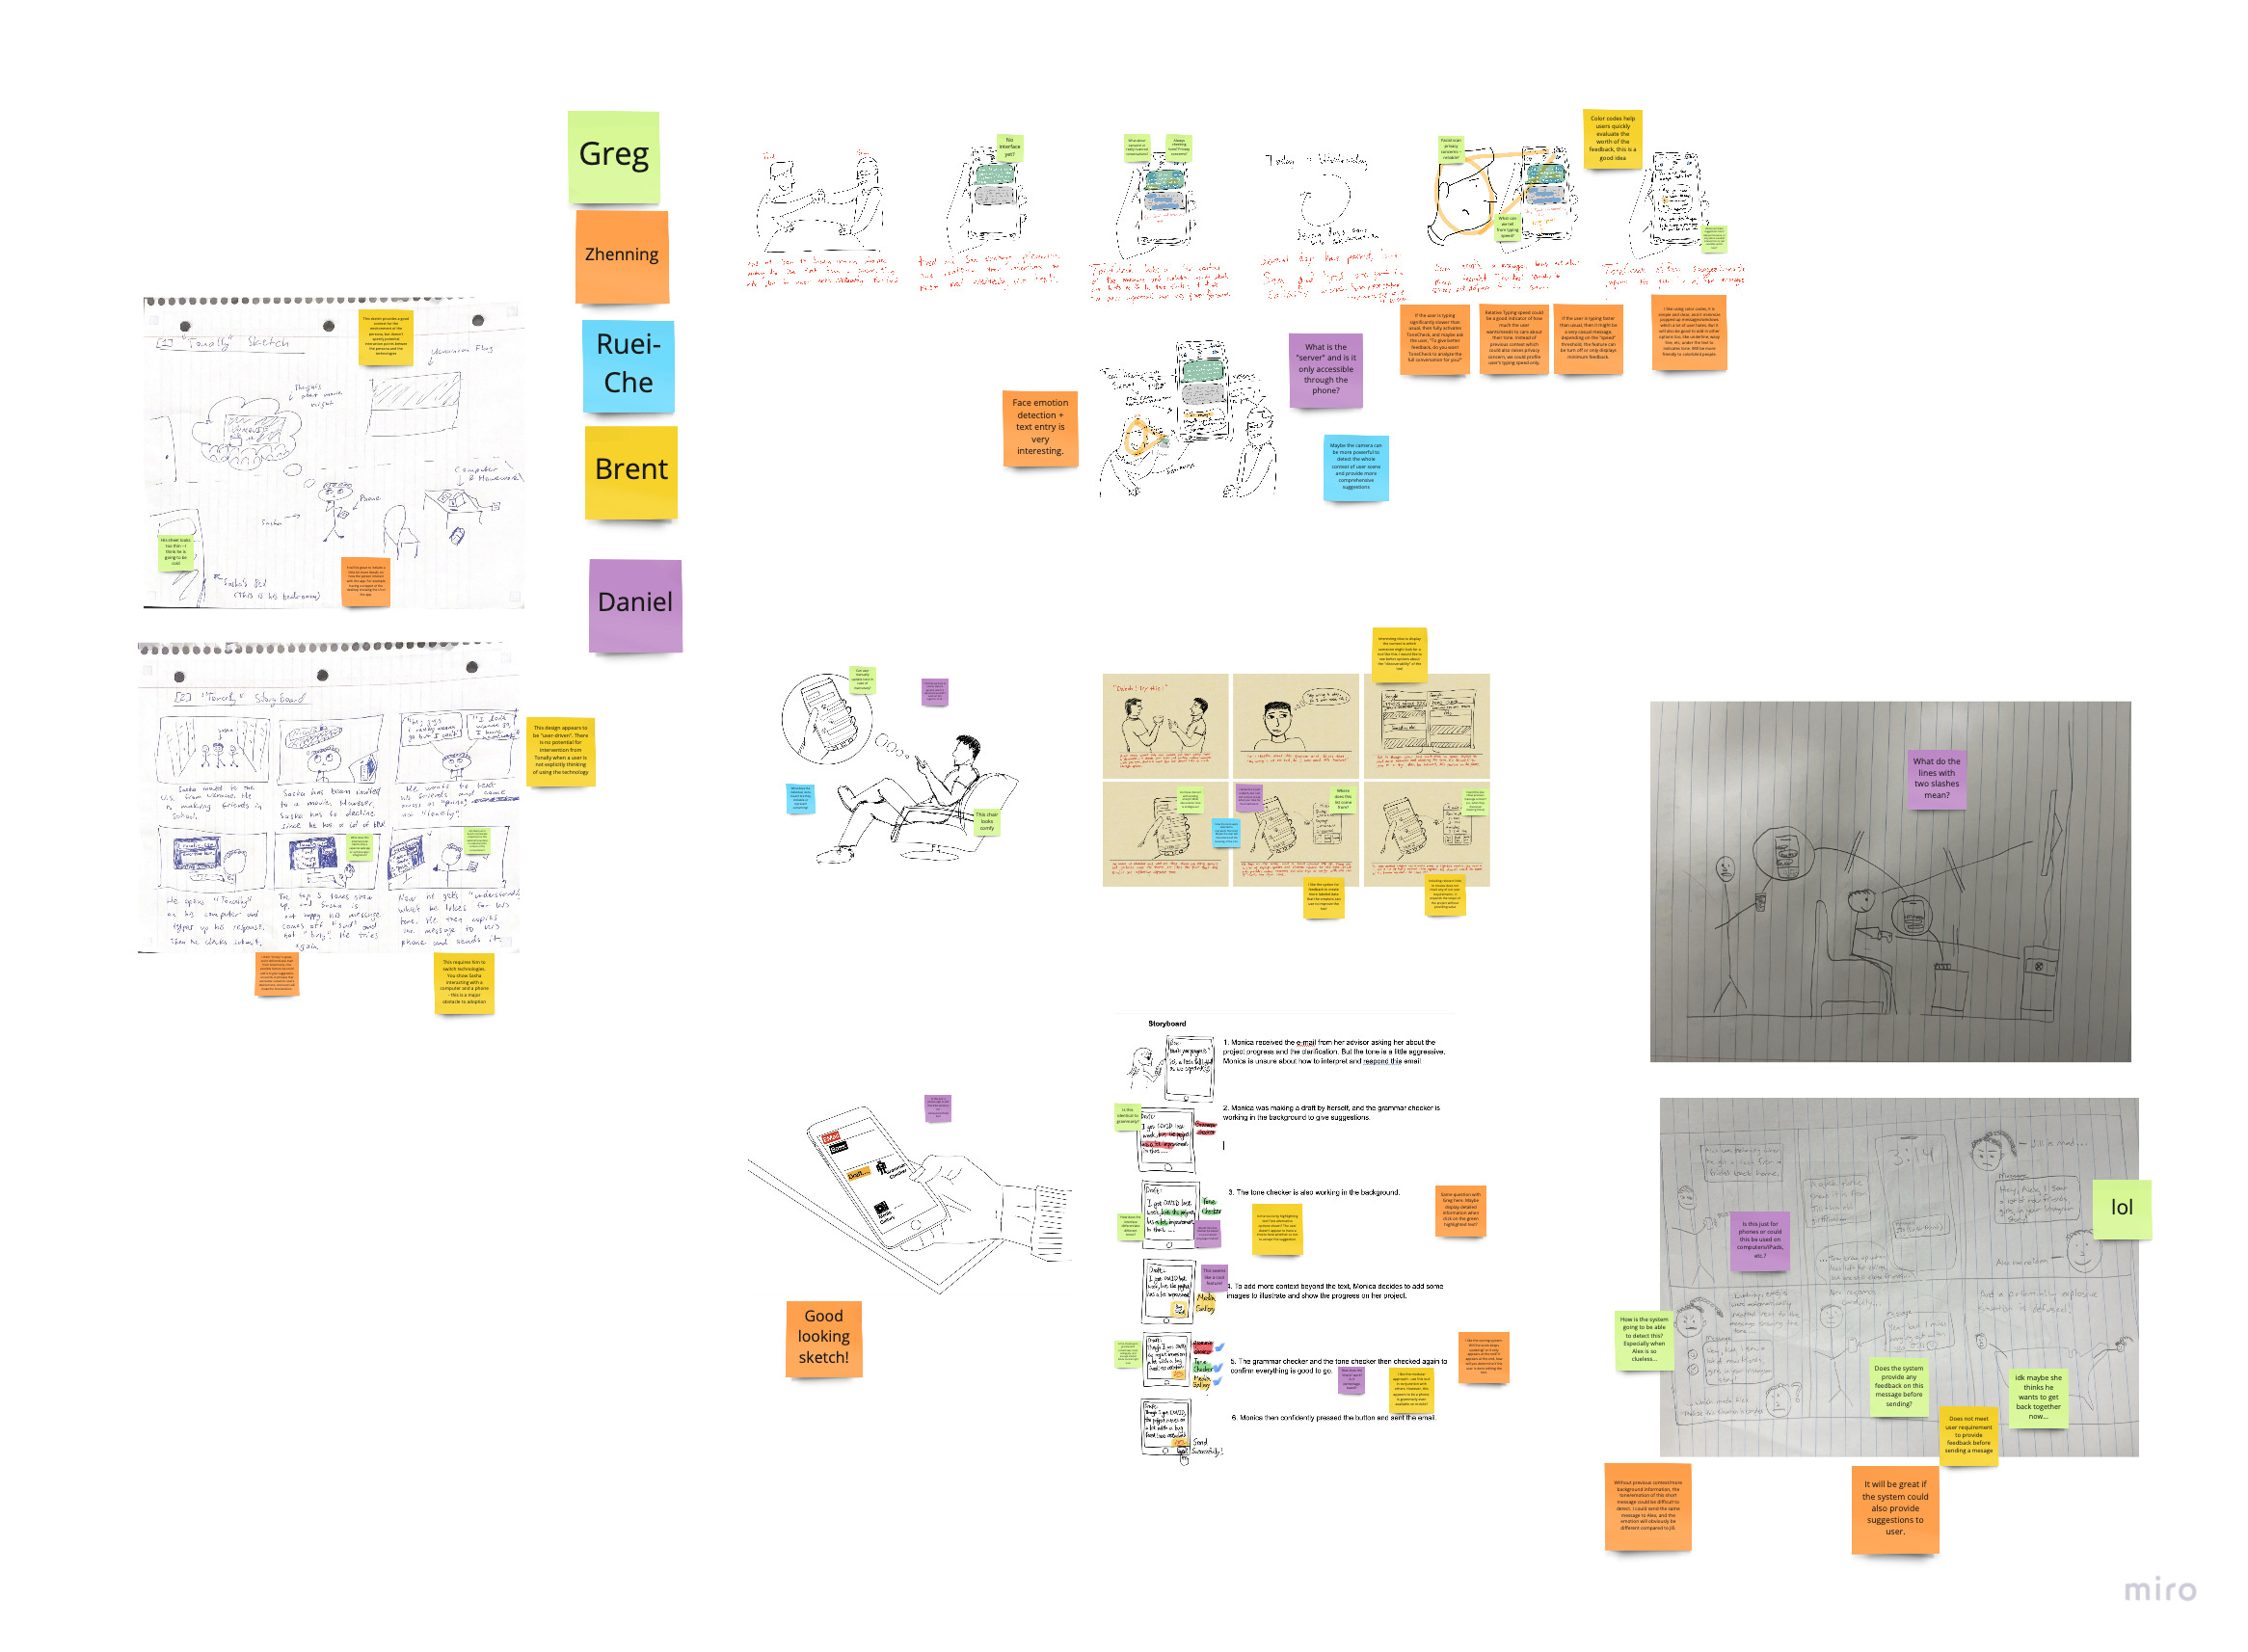
\includegraphics[width=1.0\linewidth]{figures/Assignment_3/DesignCritiques.jpg}
\caption{Miro Board which contains critiques of Individual Sketches and Initial Designs as depicted in Individual Storyboards}
\label{fig:critiques}
\Description{}
\end{center}
\end{figure*}

Initial designs were created by each team member, and a critique of designs was done through critiques of individual sketches and storyboards. The critiques were consolidated in order to form a final design, which is portrayed in a final sketch and storyboard that includes a final persona. A description of a "Wizard of Oz" prototype of our design is also listed in Section \ref{paper_prototype}.

\subsection{Personas}

Individual personas were created and are listed in Section \ref{appendix:personas}. These were consolidated into a final persona that is listed in Section \ref{appendix:final_persona}.

This final persona, Monica, is a graduate student at the University of Michigan. 
Monica, shown in Figure \ref{fig:final_persona}, is based on the individual persona described in Section \ref{indiv_persona_rc} and edited to consolidate useful parts of each of the individual personas.

Monica is a 25-year-old international graduate student majoring in computer science and engineering. She is from China. She does research for a professor and is trying to decide whether to pursue a PhD or not. She likes to play video games and go shopping with her friends. She uses English only when posed in professional settings, such as meeting with her advisors, conducting research with participants, and attending formal academic events. 

She regards herself as an open-minded and outgoing person. She is confident to be talkative with every person and tries to interact with people to understand them. However, when talking to native English speakers, her cognitive load is very high after talking for a long time. 

She regularly uses email to communicate with her professor and other researchers. She gets stressed when drafting emails, and spends lots of time revising to avoid misunderstandings.

In non-professional settings, she feels more comfortable using Chinese. She has many friends that are still living in China that she likes to talk to. Because she has been gone for so long, she only gets to use WeChat and iMessage to talk with her friends back home. Without face to face interaction, she doesn't have many emotional conversations with her friends in China, and those friendships are weaker because of it.

The online communication tools she uses are her personal iPhone and Macbook Pro. For the
app for chatting or texting, she typically uses WeChat and iPhone built-in message app. For the laptop applications, she uses Slack to communicate with labmates and folks at University, or she uses emails to communicate with people depending on others' preferences.

She is a subscriber of Grammarly to help her to correct grammar mistakes in real-time. If
Grammarly fails to provide feedback or gives ambiguous suggestions, she turns to her friends to ask if they can have a look. 

\subsection{Sketches}

Individual sketches are listed in Appendix \ref{appendix:individual_sketches}, and similarly, there were consolidated into a final sketch, Figure \ref{fig:final_sketches}. 

Based on the critiques, some sketches have too many potential platforms. For the final sketch, the team reduced information regarding the surrounding environment and platforms, instead focus on the persona and one single platform (smartphone) only. The team envisions this feature to be an add-on for any Mobile communication software; that is also extendable to other platforms later on. In the scope of this project, the final sketch depicted the persona casually sitting on a chair interacting with her phone with the feature activated. 

The snippets of the phone is depicting the general use-case of the feature where the full conversation are color-coded, and colors are mapped to tones/emotions. The team have decided to use color as default. Unlike emojis, color is able to provide denser feedback with minimum pop-up windows which could potentially disrupt the conversation. 

\subsection{Storyboards}
Individual storyboards are included in Appendix \ref{appendix:individual_storyboards}.

The design depicted in the Figure \ref{fig:storyboard_dc} included too many potential platforms. The interface for the tool was unclear, whether it was supposed to be a web or native application, or a plugin in an existing program. It was also desktop based, which produced friction when the persona wanted to have a conversation on their phone. The design was also completely user-drive, and didn't have potential for intervention when a user is not explicitly thinking of using the technology. There was also no suggestions produced for the user, which is a desirable feature.

The design depicted in Table \ref{tab:storyboard_gc} was effective due to its use of color coding. However, it is not specified when the interface will appear over a messaging app - if it is always present, or triggered. This created privacy concerns - is this app always running in the background? The color coding approach has the potential to mis-characterize a sarcastic or nuanced message - these cases require looking at the message as a whole, not just individual words. The tool also used mainly biometrics and the raw text as input. There is potential here to use metrics like typing speed - a slower relative typing speed could be an indicator of how much the user wants/needs to care about the tone of a message. Another issue with the color codes is that this would violate principles of universal design. Blind and color-blind people would not be able to use this tool, and other markers, like underlining and boldface fonts, would be more inclusive.

The design depicted in \ref{fig:storyboard_zy} included providing links to online resources and other conversations with a similar tone to allow the user to build the context for themselves. There wasn't any indication in the design as to how to navigate to this interface, which is potentially a discoverability concern. The emojis were a clear way to convey tone to our final persona, who is a millennial, but may not be easily understood by those from older generations. Additionally, this design only uses a single emoji, which may be inadequate when the tone is ambiguous or complex. The emojis were a metaphor for a button of some sort and were supposed to be pressed, however, this design didn't clearly signify that the emojis were to pressed, or what would happen if they were pressed, and the user might be confused. Finally, the design also included links to ads or to movies and other outside content that did not meet any user requirements in terms of understanding the tone of the conversation. These design features may be superfluous and could be removed to limit the scope of the final product.

The design depicted in \ref{fig:storyboard_rc} was one of the only designs to explicitly allow for interactions with other existing tools, and this was a positive. However, the design did not specify how this interaction may take place when there is a conflict. For example, what if the "tone checker" and the "grammar checker" both want to highlight a piece of text. The storyboard specifically had some ambiguity as to what was being done by outside tools, and what was being done by the design to help the persona understand the message. Additionally, this design only highlighting emotional language, without classifying it for the user.

The design depicted in \ref{fig:storyboard_bg} does not clearly define how a given message is going to be parsed - this is an implementation detail, but it important to help the persona know how to use the tool. Additionally, this design only provides simple feedback on incoming messages, but does not attempt to meet the user requirement to provide feedback on outgoing messages. 

Taking pieces of each of the prototypes and the feedback they generated, we specified a final design which color codes grammar and tonal mistakes in distinct colors (which could be replaced with emojis for the color-blind), provides content context when needed, and acts as a buffer before the final submission of a message. Figure \ref{fig:final_sketches} is a sketch of our final persona, Monica, in context of the final design. Figure \ref{fig:final_storyboard} depicts a storyboard of Monica using this design to help her avoid any misunderstanding in a text conversation with a colleague.

The captions on the final storyboard give full details of the interaction between Monica and a colleague, Sam. Monica meets Sam and has a brief text conversation with him. The design aids in understanding the beginning of this message, and also intervenes when Monica revisits the conversation after several days and drafts a follow up message.

\subsection{Paper Prototype}
\label{paper_prototype}
% Does the Initial Design and Low Fidelity Prototypes section contain a description and figures depicting the the "final" group design paper prototype? Does the description contain justification for changes based on the design critiques? Does the section contain a brief description of how an investigator could Wizard of Oz the prototype?

% \begin{figure}[H]
% \begin{center}
% \includegraphics[width=1\linewidth]{./figures/Assignment_3/paper_prototype.png}
% \caption{Final Paper Prototype}
% \label{fig:final_paper_prototype}
% \Description{}
% \end{center}
% \end{figure}

According to the individual designs and their critiques, the group has developed the final paper prototype \ref{fig:final_paper_prototype} based on the final design. We envision it as an add-on feature for communication tools such as WhatsApp, WeChat, Facebook and so on. Smartphones are used to demonstrate the usage in the final paper prototype. As mentioned before, the team reduced all potential platforms to one (smartphone), but it can be extendable to other platforms. 

Two individual designs employed color codes to indicate tones/emotions and grammar errors. This style is preferred by most group members. As the critiques suggested, emojis might be easy for millennial to understand, but may not be easily understood by those from older generations. The use of color minimized the appearance of pop-up information which can take up precious screen real-estate while still able to provide helpful signals about tone and error. Overlaying color on texts can provide very dense feedback on a message, but the control of feedback density is given to users as shown in the prototype (refer to the "Setting" screen). Color codes are activated by default when this feature is on, but colorblind users have the option to switch to emojis. 

Not to mention, user privacy was brought up by a few team members. We think that, for better performance, tone-check needs to have access to the full conversation. But to address this issue, the team decided to still add the "Privacy" section in the setting, and when it is turned off, this feature will only analyze the user's ongoing text. 

In addition to colors and emojis, when users click on the area, a little window will pop up displaying a little bit more information; the user can click on the dots, and it will switch to a different page in order to bring up even more information. For example, a sentence is classified as "happy", this sentence will be colored green, and a little window showing 1 to 2 synonyms and one quote. More synonyms, sayings, quotes, and pictures will be shown on the detailed page. 

For grammar errors, a list of suggestions will be provided, and they will replace the current text on click. This feature can also be completely turned off (refer to the last screen). Noted that this "grammar-check" is not specified in the user requirements. In the scope of this project, the main focus is "tone-check" but our implementation should not interfere with any built-in auto-correct feature. Instead, as the final paper prototype suggested, both should function in parallel. 

Before any serious implementation, this final design also can serve as a cheap, fast, and disposable prototype for users to experience. Initially, the user holds the first paper phone screen with color-coded texts, and we will hold all the other screens. The user can click on the paper phone screen, and we will hand the user the corresponding piece of paper representing the "next" screen. This will simulate user interactions with a phone so we can "Wizard of Oz" this prototype. The user's feedback will inform the team how to proceed, including potential improvements and additional iterations of prototyping. 

\section{Usability Evaluation}

\subsection{Heuristic Evaluation}

Heuristic evaluation is an essential part in the user-centered design process. To develop an effective interface, designers want to optimize usability and remove or minimize any design deficiencies. In heuristic evaluation, designers are given the opportunity to demonstrate how their low-fidelity prototype works to usability expert(s). By showcasing how we as designers expect the targeted audiences or users to interact with the design prototype in order to fulfill the selected user requirements. Feedback from usability expert(s) will expose any observed usability issues and design flaws. As a group, these valuable insights gathered from multiple experts will further inform the next iteration of the prototyping. 

\subsubsection{Method}

To perform heuristic evaluation, the team discussed and ranked the defined user requirements, then selected the top requirement(s). Each team member recruited 1 usability expert. Using the final design prototype, we each demonstrated how we expect the user to interact with this design to accomplish the goal (user requirements). Then the expert described each problem they detected based on these 10 usability heuristics: 

\begin{enumerate}
    \item Visibility of system status
    \item Match between system and the real world
    \item User control and freedom
    \item Consistency and standards
    \item Error prevention
    \item Recognition rather than recall
    \item Flexibility and efficiency of use
    \item Aesthetic and minimalist design
    \item Help users recognize, diagnose, and recover from errors
    \item Help and documentation
\end{enumerate}

Usability experts then rated each of the problems they described from scale of 1 to 5 regarding severity of the issue. 

\begin{itemize}
    \item 0 = I don't agree that this is a usability problem at all
    \item 1 = Cosmetic problem only: need not be fixed unless extra time is available on project
    \item 2 = Minor usability problem: fixing this should be given low priority
    \item 3 = Major usability problem: important to fix, so should be given high priority
    \item 4 = Usability catastrophe: imperative to fix this before product can be released
\end{itemize}

\subsubsection{Tasks and Procedures}

The team identified four tasks to perform during hueristic evaluation. The tasks are as follows:

\begin{enumerate}
    \item Review the emotional context of a message
    \item Disable Grammar checking
    \item Get tonal feedback using emojis
    \item Draft a response to an emotionally charged message
\end{enumerate}

Tasks 1-3 will use a Powerpoint slide representing possible phone screens (included in Appendix \ref{appendix:paper_prototype_slides}). Task 4 will be simulated using live-highlighting and annotation by the interviewer (on a Google doc).

The procedure is as follows:

\begin{enumerate}[label*=(\arabic*)]
    \item Gather relevant participant information.
    \item Inform the user of the general context of use and provide them with a copy of the user requirements (goals).
    \item Navigate to the SharePoint link (Appendix \ref{appendix:paper_prototype_slides}), which will be used to “Wizard of Oz” the low-fidelity prototype for Tasks 1-3.
    \item Begin on slide 1. Explain that this is an existing message thread inside a non-specific messaging app. Explain that the tool is working in the background to analyze the emotional content of the message, and has highlighted the messages based on the result.
    \item Emphasize the meaning of the colors
    \subitem Yellow is “question”
    \subitem Green is “nuanced”
    \subitem Grey is “disinterest”
    \subitem Blue is “explanation”
    \subitem Pink is “complaint”
    \item Click on one of the highlighted lines, and illustrate the change in state by changing slides to the appropriate display, where the popup provides more details on the phrase you just clicked. Read aloud the information provided, as well as the emojis included and the settings button. “Exit” the popup by clicking on any of the blank areas of the screen, which will “return” you to the main screen (slide 1).
    \item Repeat step 2 several times for different colors to illustrate this thoroughly to the expert evaluator. This will comprise Task 1.
    \item Begin Task 2 by clicking on one of the highlighted phrases, navigating to the appropriate popup slide, and then clicking the gear emoji and navigating to slide 10. Narrate the settings options available. 
    \item Click on the grammar slider, and navigate to slide 11 to show the change in state. Then click the left arrow button on the left side of the screen to exit, and return to slide 1. Explain that grammar highlighting would now be disabled (there were no existing grammar issues, so no highlighting changed).
    \item Start Task 3 by, again, clicking on a highlighted phrase, clicking on the settings button, and going to slide 10.
    \item This time, click on the color/emoji slider, and navigate to slide 12 to show that the tool is now in “emoji” mode. Click the back button, and change to slide 13 to show a sample screen of the emoji output.
    \item Shift to Task 4 by switching to the “live edit” Google Doc. Explain that the highlighting will follow a slightly different paradigm here, as this is a different prototype of the design to be used for drafting messages. In this prototype, green highlights mean a positive message, red means negative, and yellow means ambiguous/complex/nuanced. Note that this is the same conversation as the powerpoint.
    \item Read the message aloud, noting the highlighted sections. Then, begin drafting a response. 
    \item Purposely include a typo, and show how the red underline indicates a typo. Fix the typo, and explain that the tool also has a spell and grammar checker, as seen earlier in the settings screen.
    \item Type the negative response, “Well you need to get it all done.” Highlight this phrase in light red to show that it is “negative”. Comment on the live highlighting, and “click” on the phrase. Verbally explain that the popup would explicitly state that this is a negative phrase, and that the meaning/synonym of the phrase is “you aren’t doing enough.” Comment that this isn’t the message you are trying to convey, and delete your message draft.
    \item Try again to draft a message, this time typing, “That sounds really hard, what can I do?” This time, highlight the phrase in light green to show it is “positive”. Say you are now satisfied that you have drafted a message that will be received positively, and “send” it. 
    \item Continue the conversation, making up responses from the friend and drafting and live-highlighting responses, for two or three more messages.
    \item Indicate to the expert evaluator that the demo is completed. Display both prototypes (Powerpoint and Google doc), and ask them what usability problems they recognized. For each individual problem, record a detailed description, which of the 10 categories it belongs to, and the severity rating. 
\end{enumerate}

\subsubsection{Participants}
\\
% \instructions{Please provide demographic information of participants: number of participants, by age, by gender, by disability if relevant for the study, by experience with task, location, any other criteria for recruitment, how they were recruited, were they given any incentives, mode of study conducted (virtual or in-person) How was consent for participation sought and administered? How did you decide on the number of participants for your study?}
\textbf{Participant 1: }The expert participant is a current student in the class EECS 593. The expert is studying for a master’s degree in ECE and will have an engineering job in HCI Lab at Huawei after graduation. 
%rueiche

\textbf{Participant 2: }The usability expert is a first-year Master's student here at the University of Michigan, studying computer science. He interacts with technology very frequently, and is interested and keeps track of new incoming tech too. 
%ZY

\textbf{Participant 3} The expert was an 18-25 year old individual who identified as female. The highest education they have completed is a Bachelor’s degree. This individual is currently enrolled in an HCI class at the University of Michigan, and this gives them the background and expertise to be able to serve as a usability expert for this heuristic evaluation. 
% BG

\textbf{Participant 4} This expert is a first year Master's student in Computer Science at the University of Michigan, also with an undergraduate degree from the same institution. They are currently enrolled in the 593, HCI, as part of their graduate coursework. Heuristic evaluation is a core component of the course, qualifying them to participate in an expert evaluation of this interface.
% GC

\textbf{Participant 5} The participant is a first year Computer Science PhD student at the University of Michigan and is enrolled in EECS 593: HCI taught by Professor Nikola Banovic for fall 2022. Therefore, by being enrolled in this course they are able to be the usability expert to access this project.


\subsubsection{Results}

Table \ref{tab:hueristic_evaluation} summarizes the feedback received from the expert evaluators.

\begin{center}
\begin{longtable}{|l|p{0.15\linewidth}|l|p{0.6\linewidth}|}
\caption{Heuristic Evaluation Results} \label{tab:hueristic_evaluation} \\

\hline \multicolumn{1}{|c|}{\textbf{Issue \#}} & \multicolumn{1}{c|}{\textbf{Hueristic}} & \multicolumn{1}{c|}{\textbf{Severity}}  & \multicolumn{1}{c|}{\textbf{Description}} \\ \hline 
\endfirsthead

\multicolumn{4}{c}%
{{\bfseries \tablename\ \thetable{} -- continued from previous page}} \\
\hline \multicolumn{1}{|c|}{\textbf{Issue \#}} & \multicolumn{1}{c|}{\textbf{Hueristic}} & \multicolumn{1}{c|}{\textbf{Severity}}  & \multicolumn{1}{c|}{\textbf{Description}} \\ \hline 
\endhead

\hline \multicolumn{4}{|l|}{{Continued on next page}} \\ \hline
\endfoot

\hline \hline
\endlastfoot

1 & Visibility of System Status & 2 & Not evident how the tool is scraping conversation history behind the scenes, and therefore can’t build trust with tool \\ \cline{1-4}
2 & Visibility of system status & 2 & The only spot where I can see a user not immediately understanding the outcome of their interaction would be when adjusting something in the settings. For example, if one were to toggle Grammar or Tone, the effects wouldn’t be clear until the user went back to the chat screen. \\ \cline{1-4}


3 & Match between system and real world & 1 & Unsure how to immediately exit out of popups \\ \cline{1-4}
4 & Match between system and the real world & 1 & Generally speaking there doesn't seem to be any jargon that might confuse a user; however, perhaps ‘Density’ in the Settings section would not be immediately interpretable in context. \\ \cline{1-4}
5 & Match between system and the real world & 2 & The “Quote” function in our tool is confusing, as it wants to explain the targeted sentence through another’s perspective but still in an “emotional” way. \\ \cline{1-4}

6 & User Control and Freedom & 1 & Unclear how to turn the tool off. “Off” switch is buried on a settings screen \\ \cline{1-4}
7 & User Control and Freedom & 1 & the one action that is not perfectly clear right now is how a user might go back to the chat screen after going to the pop-up screen with text analysis (can they click on a blank space on the screen? Will there eventually be a back button?) \\ \cline{1-4}
8 & User Control and Freedom & 1 & It is not clear how first-time users can return to the previous page. This can be presented in the early stage first and gradually disabled once the user is familiar with it. \\ \cline{1-4}


9 & Consistency and Standard & 1 & The pop ups aren’t formatted like well known dictionaries or other common tools \\ \cline{1-4}
10 & Consistency and Standards & 1 & Emojis can be interpreted in new ways over time due to pop culture so this could add a layer of confusion.  \\ \cline{1-4}
11 & Consistency and Standards & 1 & Highlighting the entire phrase is not conventional, underlining and muted highlighting is more common \\ \cline{1-4}
12 & Consistency and Standards & 1 & Mostly good, the use of the toggle buttons and sliders are appropriate and intuitive to use in the settings screen. That being said, there’s a possibility that it could come off as confusing to have various types of buttons consecutively on that screen, especially if they’re in the same section; if Grammar and Tone don’t have the same functionality (if I misunderstood that, then disregard this!) then perhaps they should be in fully separate sections altogether.\\ \cline{1-4}
13 & Consistency and Standards & 2 & I really liked the engaging idea of using various colors to represent each tone. However, this might cause some confusion without proper user guidance since mapping the colors to tone is primarily dependent on the user's intuition. \\ \cline{1-4}
14 & Consistency and Standards & 2 & The setting icon (gear) is presented everywhere but not a fixed space that people can know where to access. \\ \cline{1-4}

15 & Error Prevention & 2 & When tapping on a highlighted phrase, room for ambiguity and mistakes. Is the user trying to enter a popup, or move the cursor to that word? \\ \cline{1-4}
16 & Error Prevention & 2 & The paper prototype lacks an error prevention feature. When the user chooses one of the synonyms from the list of recommended words, the user might make a mistake due to the size of the interface. It could be solved by using error prevention techniques (e.g., adding a confirmation to double check user’s choice, making the UI bigger …) \\ \cline{1-4}
17 & Error Prevention & 2 & With the changes that can be made in the settings, I think that these might benefit from some failsafes, or at least some pop-ups over different sections (e.g. if a user tries to toggle the Grammar section, then a pop-up can explain what that action will do and confirm if that is what a user wants as opposed to the Tone toggle button). \\ \cline{1-4}

18 & Recognition and Recall & 3 & The highlighted colors force recognition of what they mean instead of being easily recalled. \\ \cline{1-4}
19 & Recognition and Recall & 3 & The titles of the different sections of the settings are not easily interpretable right away (e.g. what does toggling the ‘Tone’ button do, especially since ‘Tone’ isn’t part of the text analysis bubble) \\ \cline{1-4}

20 & Flexibility and Efficiency of Use & 1 & For the expert user, this won’t help someone who is already in touch with the emotions of a conversation.  \\ \cline{1-4}
21 & Flexibility and Efficiency of Use & 1 & Tool doesn’t explain how it is personalizing the content/suggestions to the specific user.  \\ \cline{1-4}
22 & Flexibility and Efficiency of Use & 1 & No way to filter suggestions based on complexity - i.e. only highlight text that is higher than a certain level of emotional complexity \\ \cline{1-4}

23 & Aesthetic and Minimalist Design & 4 & The highlight colors are “awful” - jarring and distracts from the messaging app \\ \cline{1-4}
24 & Aesthetic and Minimalist Design & 3 & The popup is very intrusive in that it blocks out all the other messages on the screen. \\ \cline{1-4}
25 & Aesthetic and Minimalist Design & 2 & Scrollable box (as popup to show content) seems out of place in a messaging app \\ \cline{1-4}
26 & Aesthetic and Minimalist Design & 1 & Highlighting/indicating the entire phrase in “color mode” is excessive  \\ \cline{1-4}
27 & Aesthetic and Minimalist Design & 2 & Content within popup is uniform text size/style, which doesn’t look good or draw attention to most relevant information. \\ \cline{1-4}
28 & Aesthetic and Minimalist Design & 1 & Content categories (sayings, quote, etc) are still visible even when there is not content for that specific phrase, doesn’t need to be displayed \\ \cline{1-4}
29 & Aesthetic and Minimalist Design & 2 & The emojis are presented everywhere and their underlying meaning is confusing. The expert suggests deleting them to make the functions clear. \\ \cline{1-4}

30 & Help users recognize, diagnose, and recover from errors & 2 & I’m not sure if there’s any functionality right now to do any tutorials for users to get out an error. \\ \cline{1-4}

31 & Help and Documentation & 2 & Settings page missing a key that describes each of the settings, what colors mean, what information may be presented \\ \cline{1-4}
32 & Help and Documentation & 2 & Same issue as stated in "Error prevention", but we can also allow users to recover from the error instead of preventing it from happening. The most general way would be adding an Undo function which allows the user to switch back to the original sentence if they made a mistake. \\ \cline{1-4}
33 & Help and Documentation & 3 & No full tutorial available - should be presented at installation time or upon first use of the tool \\ \cline{1-4}
34 & Help and documentation & 1 & It is a minor issue but I think it would be helpful if there is a user guide that indicates how to interact with your software. \\ \cline{1-4}
35 & Help and documentation & 2 & The meaning behind each color is unclear and can be added to the instruction page. \\ \cline{1-4}
36 & Visibility of system status & 2 &  No way to see how close to being completed the tone checker is. \\ \cline{1-4}
37 & Match between system and the real-world & 1 & Explain what synonym is. \\ \cline{1-4}
38 & Match between system and the real-world & 1 & Change the “Sayings” to be “Simplified” for better clarification of what the phrase actually means. \\ \cline{1-4}
39 &  User control and freedom & 3 & Add a backspace option on any of the pop ups as seen in slides 2-9. \\ \cline{1-4}
40 &  User control and freedom & 1 & Maybe make the setting page swipeable at all times (instead of it being a button or swipeable) for consistency. \\ \cline{1-4}
41 & Consistency and standards & 1 & Add dictionary mode for individual words. \\ \cline{1-4}
42 & Error prevention & 3 & Add “error reporting” function (where the user can report to someone if a “synonym” or “simplification” if it doesn’t seem correct). \\ \cline{1-4}
43 & Recognition rather than recall & 1 &  Include a tutorial for what different colors mean for first time users of app (like how Google does it first time you open email, docs, etc.). \\ \cline{1-4}
44 & Flexibility and efficiency of use & 2 & Have a swipe left/right function to go to the last/next highlight. \\ \cline{1-4}
45 & Flexibility and efficiency of use & 2 & Have a function to “unhighlight” if the user doesn’t feel like they want see the specific highlight/declutter the screen option. \\ \cline{1-4}
46 & Aesthetic and minimalist design & 1 & Get rid of the “Quote” feature (doesn’t seem to add anything). \\ \cline{1-4}
47 & Aesthetic and minimalist design & 1 & Same with emojis (also emojis don’t always appear on all phones). \\ \cline{1-4}
48 & Help users recognize, diagnose, and recover from errors & 2 & Add question marks into different places that can be grounded into different contexts (so there aren’t any intersecting opposing tones). \\ \cline{1-4}
49 & Help and documentation & 2 & Have a question mark on the setting page that reviews the demo that shows for first time users. \\ \cline{1-4}
50 & Help and documentation & 2 & Include searching FAQs and commonly asked questions pop up from the settings page. \\ \cline{1-4}

\end{longtable}
\end{center}

\subsection{Simplified User Testing}

Simplified User Testing is a method which enables researchers to testify if their solution could actually satisfy their user requirements, using less effort, resources, and time into the design and implementation of the prototype. At this stage of our design process, there is still a likelihood that the prototype cannot meet the requirements and target user scenarios. Therefore, low-fidelity prototyping is an ideal proxy to ensure the path that the researchers are conducting is on the right track. After completing the user testing, the researchers will know the insufficiency of the current functionalities of the prototype and then driven by these insights, the researchers can then develop the next iteration of the prototype, which is likely of a higher fidelity.

\subsubsection{Method}

For the simplified user testing, each researcher in our team presented the paper prototype in powerpoint form (Appendix \ref{appendix:paper_prototype_slides}) to a non-expert user to see how the users interact with the prototype and testify if the proposed solutions have addressed it, and will end up with five participants in total as a group. Specifically, as we presented the low-fidelity paper prototype, each researcher will act as a “wizard” to simulate the functionalities manually. The starting screen was first presented, and we asked users to try to accomplish the tasks and achieve our goals during the experiment. The users were asked to follow the think-aloud protocol to provide their thoughts of each step in time. If certain actions would change the output of the screen, the presenter would navigate to the appropriate slide to show this to the participants.

\subsubsection{Tasks and Procedures}

The tasks for the users are as follows:

\begin{enumerate}
    \item Navigate the UI
    \item Draft a response to the existing text message
\end{enumerate}

The procedure for simplified user testing was:

\begin{enumerate}
    \item We notify our participants of the purpose and method of this experiment and the goals to accomplish, and remind them that only de-identified information will be collected. We then also let them know they can quit at any time and that they are in no way obligated to stay to complete the usability test if they do now wish to do so.
    \item The researcher next informs the user of which task they will try to complete: the navigation of the UI task (using the slides), and then as a text message responder (using the word document). Also remind them to perform think-aloud (verbalize their thoughts while interacting with the prototype) and let them know you will be able to answer simple clarifying questions but nothing more until after the usability study is complete. 
    \begin{enumerate}[a]
        \item It’s important to note here that since our prototype isn’t functional, the researcher will “Wizard-of-Oz” the functionality of the current design, using the low-fidelity design prototype, while the user attempts to complete the task. Two of our contexts of use will be used.
        \begin{enumerate}[i]
            \item Upon navigation to a conversation page, users need convenient access to information about the emotional context and content from the previous messages.
            \item After composing a message, users need preemptive feedback on the emotional tone of their draft message in the context of the previous conversation, prior to the message being sent.
        \end{enumerate} 
    \end{enumerate}
    \item For the first task, navigate to the SharePoint link, which will be used to “Wizard of Oz” the low-fidelity prototype for Task 1. Here, use the first slide with the messages as the starting screen. Tell the participant that if they wish to click on anything, to move their mouse over it and verbally say “I am clicking on [whatever they are clicking on].” Likewise, if the user is swiping in any direction, they will verbally say “I am swiping left.” or “I am swiping up.”, etc. This will then give the interviewer the opportunity to “Wizard of Oz” and open the subsequent slide based on what the user clicked on/swiped.
    \begin{enumerate}[a]
        \item Explain that this interface is like an iPhone/Android phone and that anything can either be clicked on or swiped.
        \item If certain actions would change the output of the screen, the presenter will navigate to the appropriate slide to show this to the participants.
        \item Record any difficulties users encountered and errors they make.
        \item Make sure the users are following the think-aloud protocol to provide their thoughts of each step in time. 
    \end{enumerate}
    \item For the second task, navigate to the Google Docs link, which will be used to “Wizard of Oz” the low-fidelity prototype for Task 2. Here, use the first text blurb as a message from a friend on a phone text message interface. Tell the participant that they can type up a response as they normally would: a response that doesn’t need to be grammatically correct or overtly formal. Tell the participant that while doing so our tool will have the interviewer “Wizard of Oz” the word highlighting functionality into the message as the participant types it in.
    \begin{enumerate}[a]
        \item Explain that the word document functions as a “text box” on a phone and that the user can type in a response they normally would to their friend on a phone.
        \item Record any difficulties users encountered and errors they make.
        \item Make sure the users are following the think-aloud protocol to provide their thoughts of each step in time.
    \end{enumerate}
    \item Once the simplified user testing is complete, indicate to the participant that the test is complete and thank the participant for their time.
\end{enumerate}

\subsubsection{Participants}
% \instructions{Please provide demographic information of participants: number of participants, by age, by gender, by disability if relevant for the study, by experience with task, location, any other criteria for recruitment, how they were recruited, were they given any incentives, mode of study conducted (virtual or in-person) How was consent for participation sought and administered? How did you decide on the number of participants for your study?}

\textbf{Participant 1:} The participant is a female student in a Master's Degree program to become a nurse practitioner. They are in the 18-25 age range, and regularly uses a mobile phone to access multiple platforms where they have non-professional conversations with other individuals. They are a native English speaker.

\textbf{Participant 2:} The participant is in the 18-25 age range, and is a male international undergraduate student. He is a native Chinese speaker with fluent non-native English ability.

\textbf{Participant 3:}
This participant is a male, 2nd year PhD student at the University of Michigan. He interacts with technology frequently, he sends and receives many messages everyday, and he uses WeChat as his main communication tool. The user is not a native English speaker, and they pay extra attention to their messages before sending them. 

\textbf{Participant 4:} %rueiche
The participant is female and aged 24. She is an international student from China and fluent in English. She is currently studying computer science and engineering and does not know usability and usability heuristics. She uses Wechat and some message apps, like Telegram and Gmail. 

\textbf{Participant 5:} %dchechel
The participant for the simplified user testing is a 22 year old female Kazakh, Russian, and English speaker who has been living in the U.S. for the past 4 years. She currently works at a tech-start up in Minneapolis and regularly uses Slack and iMessage for communication with coworkers.

\subsubsection{Results}

The results for simplified user testing are encoded in Tables \ref{tab:SimpUser1Task1}, \ref{tab:SimpUser1Task2}, \ref{tab:SimpUser2Task1}, \ref{tab:SimpUser2Task2}, \ref{tab:SimpUser3Task1}, \ref{tab:SimpUser3Task2}, \ref{tab:SimpUser4Task1}, \ref{tab:SimpUser4Task2}, \ref{tab:SimpUser5Task1}, and \ref{tab:SimpUser5Task2}.

\begin{center}
    \begin{longtable}{|p{0.75\linewidth}|p{0.2\linewidth}|}
    \caption{Participant 1 UI Navigation}
    \label{tab:SimpUser1Task1}
    
    \hline \multicolumn{1}{|c|}{\textbf{Utterance/Interpretation}} & \multicolumn{1}{c|}{\textbf{Action}} \\ \hline 
    \endfirsthead
    
    \multicolumn{2}{c}%
    {{\bfseries \tablename\ \thetable{} -- continued from previous page}} \\
    \hline \multicolumn{1}{|c|}{\textbf{Utterance/Interpretation}} & \multicolumn{1}{c|}{\textbf{Action}} \\ \hline 
    \endhead
    
    \hline \multicolumn{2}{|l|}{{Continued on next page}} \\ \hline
    \endfoot
    
    \hline \hline
    \endlastfoot
    
    \hline
    The participant was presented with slide 1. The participant read the entire conversation aloud, and then made a mistake by trying to scroll on the screen, when it was already at the bottom of the interface and there was no new content to scroll to. & Skimming conversation thread \\ \hline
    The participant then tried to exit the conversation by swiping up on the screen. They didn’t recognize that there was a way to interact with the highlighted text. They then re-entered the conversation, and wondered why there are colors all over the screen. & Exiting and re-entering app \\ \hline
    The participant then attempted to guess on their own what the colors meant. They came up with the following categories: questions are yellow, ellipses are green, complete sentences are purple, incomplete sentences are blue, bad grammar is gray. The participant was incorrect in inferring category types for all colors except for yellow. & Inferred meaning of color highlights \\ \hline
    The participant then clicked on “How are you”, and the researcher navigated to slide 2. The participant read each line of the content, specifically noting that they appreciated the quote. After reading all of the text, the participant recognized that the popup is telling them what the highlighted phrase means. This means that through self-discovery, the participant noted the tool’s use is to provide “convenient access to information about the emotional context and content from the previous messages,” as specified in the user requirement. This shows the participant at least recognized one of the user requirements the tool is attempting to meet. & Clicked highlighted message and read popup \\ \hline
    The participant wondered what the settings button does. They clicked on the button, and the researcher switched to slide 10. The participant scanned through the options in the settings. They were confused by the color button and weren’t sure what its functionality would be. Their first assumption was that it was an on/off switch for the entire tool, but then they re-read the text and realized it toggled between color and emoji. They were also confused by the density setting. They recognized that it was a slider and could be dragged from left to right, but didn’t read the small explanatory text, and weren’t sure what its functionality would be. They were also confused by the on/off switch, and weren’t sure what its functionality would be. They guessed that the on/off switch would have the same effect as the privacy switch, but then didn’t understand why there would be two settings for one thing. This made them guess that the two switches controlled two different settings, but they didn’t know what those settings would be. & Navigated to and explored settings page \\ \hline
    The participant then clicked on the color/emoji toggle, which changed the state and went to slide 12. The participant then was confused how to exit settings. The participant made a mistake and clicked the gear button to try to exit, but it didn’t do anything. They then clicked the left button on the side of the screen, and it navigated back to the original conversation on slide 13. & Exited settings page \\ \hline
    The participant then guessed that the colors are associated with different types of emojis. The participant clicked on the mad face emoji, which navigated to slide 7. The participant verbally expressed appreciation for the quote and found it helpful, meeting the user requirement that “users need convenient access to information about the emotional context and content from the previous messages.” & Assessed meaning of emojis and clicked on one \\ \hline
    The participant clicked on settings button, which navigated to slide 10. They commented that they expected the slides to be different, but it’s the same settings screen. They clicked on the off switch, and then clicked on the back button. There wasn’t an existing slide to demonstrate this behavior, so the researcher described that all the highlighting would disappear. The participant interpreted this as the “master on off switch”. They then wanted to turn the tool back on, but didn’t see any way to do that natively in the messaging app. After being stuck in this state for a while, the researcher navigated to slide 11 and commented that the design was incomplete and led to the participant getting stuck in an undesirable state. & Explored more settings and found some lacking features in prototype \\ \hline
    The participant then clicked on a highlighted section, which went to slide 2, and then clicked on the settings gear, which went to slide 10. The participant clicked the privacy switch, and then the back button which went to slide 1. They were surprised that the interface was the same because they were expected there to be a visual difference. (Note: after the testing was complete, the researcher explained the purpose of the privacy toggle and how the difference would be only apparent on the backend, and that the quality of the tool’s results would ultimately be the only difference, i.e. no visual difference in the interface). & Explored "Privacy" setting functionality \\ \hline
    The participant clicked the back button and went to slide 1. They then clicked on the grey highlighted text, which took them to slide 4. They made a mistake by clicking on the emoji in the top left expecting something to happen, but nothing happened. & Made an error (mistake) and clicked on emoji in popup \\ \hline
    The participant then tried to go back to the main page, but this was the first time going back to the main page in a pop-up screen. All previous attempts to return to the main conversation were from the settings screen. The participant was influenced by the layout of the settings page, so they were looking for a back arrow on the pop-up page. However, there was no arrow, so they weren’t sure what to click. They tried clicking on a blank area of the screen on the top right, which took them back to slide 1. They wanted to continue to experiment with navigation, so they clicked on the grey text again to go to slide 4, and this time they clicked a different blank area of the screen, which again returned them to slide 1. In this way they discovered how to exit the pop-up view. & Discovered how to exit a pop-up view \\ \hline
    At this point, while viewing the main page, the participant had a verbal realization that the color highlighting is associated with the emotional tone of the phrase. They wanted to go to settings to verify their understanding. They navigated to the settings page, turned off tone, and saw that highlights disappeared, and only grammar/spelling issues were underlined. This verified their understanding, so she turned the tone toggle back on in the settings page and went to the main screen. & Made the connection that color highlighting is associated with emotional tone of the phrase \\ \hline
    The participant then clicked on blue highlighted text, which navigated to slide 6. The calendar emoji had a “31” on it, and the participant interpreted the number in the calendar to be how many days ago their last conversation was. This was a mistake - it is just the default calendar emoji. & Participant mischaracterized the meaning of a helper emoji. \\
    \end{longtable}
\end{center}

\begin{center}
    \begin{longtable}{|p{0.75\linewidth}|p{0.2\linewidth}|}
    \caption{Participant 1 Typing a Message}
    \label{tab:SimpUser1Task2}
    
    \hline \multicolumn{1}{|c|}{\textbf{Utterance/Interpretation}} & \multicolumn{1}{c|}{\textbf{Action}} \\ \hline 
    \endfirsthead
    
    \multicolumn{2}{c}%
    {{\bfseries \tablename\ \thetable{} -- continued from previous page}} \\
    \hline \multicolumn{1}{|c|}{\textbf{Utterance/Interpretation}} & \multicolumn{1}{c|}{\textbf{Action}} \\ \hline 
    \endhead
    
    \hline \multicolumn{2}{|l|}{{Continued on next page}} \\ \hline
    \endfoot
    
    \hline \hline
    \endlastfoot
    
    \hline
    The participant read the existing message thread, which exactly matched the messages in the slides in the Appendix. The participant then drafted a message,  “I’m sorry, that must be really hard for you”. “I’m sorry” was highlighted in green, which indicated a positive tone. The participant was confused why it was highlighted green since they don’t perceive that phrase as positive. & Participant drafted and sent initial reply. \\ \hline
    The researcher typed a response, “I’m going to go away, don’t feel like eating”. Most sections of the response were highlighted in red, indicating a negative tone. The participant said the other person sounded depressed, and didn’t comment on or notice the highlighting at all. & Participant ignored syntax highlighting on incoming message. \\  \hline
    The participant drafted and sent a message, “Can I bring you over dinner, that way food is taken care of?” A section of the draft was highlighted in green, but was not used or noticed by the participant. & Participant drafted and sent another reply. \\ \hline
    The researcher typed a response, “No, there isn’t much anyone can do”, which was highlighted in red as a negative phrase. That participant commented, “I’d be really concerned for this person because of the previous two comments, they sound hopeless, but eating isn’t a hallmark sign of depression." At this point, the participant indicated they would not reply to the text conversation, even to ask if they are doing okay. They said this is because this conversation is one of those conversations you need to have over the phone or in person because there is a lot of emotional complexity.  & Participant chose not to respond anymore. \\  \hline
    The participant commented that the answers are really broad, and the participant isn’t sure what the responses mean. “Not much anyone can do” could be laughing it off, or could be hopeless. Not wanting to eat could mean they just ate and aren’t hungry anymore, or it could be they aren’t taking care of themselves. The participant isn’t sure what is meant, and has zero trust in the tool to augment the understanding. & Participant is unsure how to evaluate the entire conversation \\ \hline
    The participant actively ignored highlighting of message drafts and responses and relied on their own intuition to interpret the emotional context of the phrase. The participant evaluated their emotional IQ and determined that it was higher than the tool, and didn’t trust the tool to provide any additional information on the conversation. The highlights indicated that all of the responses were negative, but the participant decided that this could have been an overreaction, and that information not contained in the text conversation was essential to determine the true emotional context of the message. In this way, the design succeeded in providing feedback and information on the emotional context of the message, so it technically met the user requirements. However, this feedback and information was deemed irrelevant and useless. The design also failed to provide an opportunity to explicitly prompt the user to include pictures or emojis in the text message, so it failed to meet that user requirement. & Participant ignored the tool's highlighting at all stages of conversation \\ \hline
    \end{longtable}
\end{center}


\begin{table}[H]
    \begin{tabular}{|p{0.5 \linewidth}|p{0.5 \linewidth}|}
    \hline
    Utterance / Interpretation                                                                                                                                                                                    & Action                                  \\ \hline
    The start screen is a generic messaging screen which the participant was familiar with, but the colors had no explanation or guide to go along with them, so the participant was confused right out the gate. & Evaluated start screen                  \\ \hline
    After experimenting with the interface a little bit, the participant clicked the highlighted message, without expecting much to happen. Participants definitely need more guidance in the future.             & Clicked highlighted message             \\ \hline
    The tooltip contained a lot of information which was not presented hierarchically, so the participant indicated that they were confused by the content and did not know what was important.                   & Evaluated tooltip                       \\ \hline
    Again, after experimentation, the participant clicked on the small gear button. After this interaction, they indicated that this button was very small and hard to notice.                                    & Clicked settings button                 \\ \hline
    After evaluation of the settings interface, the user toggled the grammar setting, but seemed unsure what it would do, as grammar-checking is not well indicated in the aforementioned interface               & Toggled grammar setting to off position \\ \hline
    \end{tabular}
    \caption{Participant 2 UI Navigation}
    \label{tab:SimpUser2Task1}

\end{table}[H]
    \begin{table}
        \begin{tabular}{|p{0.5 \linewidth}|p{0.5 \linewidth}|}
        \hline
        Utterance / Interpretation                                                                                                                                                                                                             & Action                                    \\ \hline
        This demo included a very brief and clear mapping, so the color associations were much easier for the user to understand.                                                                                                              & Saw previous message with tonal highlight \\ \hline
        The user was familiar with how to interact with this demo, so this action and task were fairly straightforward.                                                                                                                        & Composed new message                      \\ \hline
        After drafting the message, the user looked at the realtime tonal analysis of what they had written. In this simple example, it was fairly straightforward and the user understood and agreed with the tonal feedback they were given. & Evaluated tonal analysis of new message   \\ \hline
        After they were comfortable with the content and tone of their message, the user sent the message with confidence.                                                                                                                     & Sent new message                          \\ \hline
        Messages were exchanged, all with similar success and utterances as had in the first case. The tonal analysis was simplified for this task, but the participant still found it useful.                                                 & Had conversation                          \\ \hline
    \end{tabular}
    \caption{Participant 2 Typing a Message}
    \label{tab:SimpUser2Task2}
\end{table}

As a reminder, the three selected user requirements were: 

\begin{enumerate}
    \item “Upon navigation to a conversation page, users need convenient access to information about the emotional context and content from the previous messages.”
    \item “After composing a message, users need feedback on the emotional tone of their draft message in the context of the previous conversation, prior to the message being sent.”
    \item “After drafting a message, users need additional ways to enhance the textual content of a message (i.e., emoji, images, emotional indicator, etc.) in order to deliver their intent unambiguously.”
\end{enumerate}

As it relates to Tables \ref{tab:SimpUser2Task1} and \ref{tab:SimpUser2Task2}, the user experienced information overload two times, dense tone/emotion information was provided to the user, however, the user did not obtain an overall tone/emotion of a message. And users tend to forget the mapping between color and tone. Hence, this design fails to meet the first user requirement. 

In terms of the 2nd and 3rd requirements, the user was able to get feedback while typing, and have easy access to resources that help refining their text. A downside is that the user also wanted suggestions on how to switch from one tone to another. Overall, this design met the 2nd user requirement and part of the 3rd requirement. 

\begin{table}[H]
\begin{tabular}{|p{0.5 \linewidth}|p{0.5 \linewidth}|}
\hline
Utterance / Interpretation                                                                                                                                                                                             & Action                                                                                      \\ \hline
User mentioned that it is hard to remember the color codes for each tone/emotion. “There are too many of them, and the color-tone mappings are not very intuitive to me”                                               & The user looked at the conversation                                                         \\ \hline
The user was not sure if the text was clickable or not. “So do I click on the colored text? Or the message box”                                                                                                        & The user clicked on one of the color-coded text                                             \\ \hline
There is too much information for each message. And he said that he doesn’t need coloring for every single phrase and sentence. Instead have one color for a message capturing the overall tone/emotion will be enough & The user clicked on a different color-coded text                                            \\ \hline
He asked why do we need sayings and quotes for the received messages                                                                                                                                                   & User is scrolling through the content within the popup windows                              \\ \hline
He said that the setting page looks okay, but there should be an easier way for users to navigate to “setting”.                                                                                                        & User noticed the “little wheel” on the top right corner, he clicked. The setting page popup \\ \hline
He said he prefers emoji mode, since they are not as dense as color, and they are easier to understand. “Emojis are easy to understand!”                                                                               & User switch to emoji mode, and clicked “go back” which brought him back to the chat room    \\ \hline
\end{tabular}
\caption{Participant 3 UI Navigation}
\label{tab:SimpUser3Task1}
\end{table}

\begin{table}[H]
\begin{tabular}{|p{0.5 \linewidth}|p{0.5 \linewidth}|}
\hline
Utterance / Interpretation                                                                                                                                                                                                                   & Action                                                                                                         \\ \hline
User was once again overwhelmed by the dense coloring. “I don’t think all these colors are helpful, having 1 tone pre message is enough, or having a progress bar on top showing the tone change throughout this conversation will be cool!” & The user looked at previous conversation                                                                       \\ \hline
“I guess I will have to delete it and rewrite the text. It will be great if it provides suggestions that can switch from one tone to another”                                                                                                & The user typed out a few words, color appeared, and the tone was not what the user wanted                      \\ \hline
“I think I wanted to express this in a different way, maybe I can look at the information from the popup window”                                                                                                                             & The user finished typing and clicked on a colored text, and found a good saying that conveys the same meaning. \\ \hline
“Wow, okay. This is pretty cool!”                                                                                                                                                                                                            & The user clicked on the saying and it replaced the original text he had                                        \\ \hline
Message sent                                                                                                                                                                                                                                 & The user clicked the “send” button                                                                             \\ \hline
\end{tabular}
\caption{Participant 3 Typing a Message}
\label{tab:SimpUser3Task2}
\end{table}





% participant #4
\begin{table}[H]
\begin{tabular}{|p{0.5 \linewidth}|p{0.5 \linewidth}|}
\hline
Utterance / Interpretation & Action                                               \\ \hline
The user is still not clear about the color codings, even we have explained. ``What does the color mean? Is there any place I can find the explanation?'' & Looking at the message thread and doing nothing.                                  \\ \hline
The most important UI element is missing and user cannot proceed if they want to message someone. ``Where is the text area that I can input the text?'' & Looking at the message thread.              
\\ \hline
The highlighted color are cues for the users to access more information. ``I want to press the highlighted text to see if any information will be provided.'' & Trying to touch the highlighted text.
\\ \hline
The user think all the highlighted text should be provided in the same page instead of the separated ones that create efforts to explore them all. ``In this page, it is supposed to be all information regarding to the highlighted text, not just the one I clicked.'' & Looking at the second page and doing nothing. 
\\ \hline
The app failed to provide the button or other information to let the user go back to the previous page. ``How can I return to the previous page?'' & Looking at the second page and looking for something.    \\ \hline
\end{tabular}
\caption{Participant 4 UI Navigation}
\label{tab:SimpUser4Task1}
\end{table}


\begin{table}[H]
\begin{tabular}{|p{0.5 \linewidth}|p{0.5 \linewidth}|}
\hline
Utterance / Interpretation & Action                                               \\ \hline
The real-time highlighted color of grammar and tone checker is distractive when the user is typing. ``The real-time highlighted color is annoying and disrupting, I really want to turn it off.'' & Typing on the device.                                  
\\ \hline
The emoji mode in our tone checker is conflicting to the user-typed emoji. ``The emojis are really confusing and conflicting to the emoji I want to type in my messages.'' & After turning the color into the emoji mode.
\\ \hline
The much information provided to the user is not always useful in certain contexts. They want to have the agency control to customize the information they want. ``I don’t think the information of quote and sayings are necessary. Synonyms are good as I can switch to other sentences and understand the diverse usage. I want to go to the setting and disable this unnecessary information.'' & Looking into one highlighted sentence, and trying to customize the settings.
\\ \hline
\end{tabular}
\caption{Participant 4 Typing a Message}
\label{tab:SimpUser4Task2}
\end{table}

\begin{table}[H]
\begin{tabular}{|p{0.5 \linewidth}|p{0.5 \linewidth}|}
\hline
Utterance / Interpretation & Action                                               \\ \hline
The user was first considering where
to click and then ultimately decided to
click on the first yellow highlight to see what happens. '' & The user wasn’t immediately certain
that they could click on the highlight.
Once clicked, it opened the pop-up.
\\ \hline
The user asked what the emoji in the
top left meant. They tried to click on it
but nothing happened. '' & The user wasn’t immediately certain
that they could click on the highlight.
Once clicked, it opened the pop-up. The emoji doesn’t act as a representation
of the highlight and instead appears as a
functional button.
\\ \hline
The user reads aloud through the
explanation of “synonym” and
“sayings” and “quotes” and agrees
that they help clarify the initial
highlighted question. '' & The “synonym”, “sayings”, and “quotes”
components somewhat accurately represent
what they say they do.
\\ \hline
The user tries to exist but then is not
able to find a way to exit out of the
pop-up. '' & Our app is currently missing a backspace
button and as such the user is not able to exit
once they enter a pop-up.
\\ \hline
The user then tries to look at other
highlights and notes how the different
colors are helpful in visualizing
different meanings. '' & The colors are a decent way to visually
represent the tones of the text messages.
\\ \hline
The user then swiped left to see the
settings page, where they noted that
there were a lot of options and toggled
them on/off upon which nothing
ultimately happened. '' & Even within our prototype, while the
settings page is in itself functional. The
various settings themselves still need to be
designed and thought about more before
implementing them to see how they function
together/separately.
\\ \hline
\end{tabular}
\caption{Participant 5 UI Navigation}
\label{tab:SimpUser5Task1}
\end{table}

\begin{table}[H]
\begin{tabular}{|p{0.5 \linewidth}|p{0.5 \linewidth}|}
\hline
Utterance / Interpretation & Action                                               \\ \hline
The user was initially thought through
the context of the previous message
and thought aloud several ways they
could respond before actually
beginning to type. `` & Might be helpful to have an
initial “starter phrase” that
matches tone of previous
message to help direct user.                                 
\\ \hline
The user began typing and
while doing so, noticed how
the highlight kept switching
colors was a little distracting to
their thought process.'' & The user is already thinking about what
they are typing so the kaleidoscope of colors
in front of them might distract them from what
they are trying to say. Perhaps the highlight
can be applied only once the person typing
stop for more than 5 seconds, for example.
\\ \hline
The user also noticed while
typing that the emoji pop-ups
were quite distracting and
sometimes were flat out wrong
(even the tone of the Wizard of Oz interviewer wasn’t always
matching what the user
intended).'' & The emoji pop ups are also distracting and
might need to be entirely scrapped since they
seem to distract more and their meanings are
in the end still vague/can be wrong.
\\ \hline
\end{tabular}
\caption{Participant 5 Typing a Message}
\label{tab:SimpUser5Task2}
\end{table}


\section{Final Design and Functional High-Fidelity Prototype}
\label{sec:final_design}
% Does the assignment contain a quality description of the changes to the design based on feedback from the qualitative evaluation? Does the assignment contain a quality description of the prototype together with screenshots of the prototype? Does the assignment contain a brief description of how the user would interact with the final prototype?

The team implemented a functional high-fidelity prototype using Figma. Figma is a template design app that lets us create a UI (User Interface) for the front end of our project design. As iMessage is a frequently-used message app by many iPhone users, we adopted an iMessage template for fast prototyping. 

Based on the results we gathered from simplified user testing, many users complained that too many colors are distractive and that most information in the popup windows is not useful and overwhelming. In our final iteration of the prototype, instead of having multiple tones/emotions for each sentence and phrase, we only indicate an overall tone/emotion per message. Popup windows are thus removed from our final design; the “popup” mechanism is now embedded into the keyboard area. The amount of information is also reduced to maintain clarity, and we envision that users should have the freedom to configure the information presentation that best suits their needs or style. People who love sending memes could configure it to only display relevant memes, as shown in the figure below. In addition, some users mentioned that the mapping between color and emotion is easy to forget. The team did some Google searches and reduced, we adopted a map that is widely used and intuitive. It contains 6 colors and emotions, and the team also added a mechanism that could remind users of the mapping. So now when a user clicks on the colored text, the mapping will appear at the bottom. The user is allowed to click the color palette for further information or return to the keyboard view by clicking the text entry box. This color palette can also serve as entries for information that is correlated with different emotions. 

Once the design is finalized, we utilized Figma’s “prototype” feature and created a custom “prototype” flow to mimic the user’s interaction on the smartphone. This functional high-fidelity prototype can be run on a smartphone with Figma mobile app installed. Figure \ref{fig:figmaprototype} shows this high-fidelity prototype, along with interaction arrows showing how click and drag actions will navigate between screens.

\begin{figure}[H]
\begin{center}
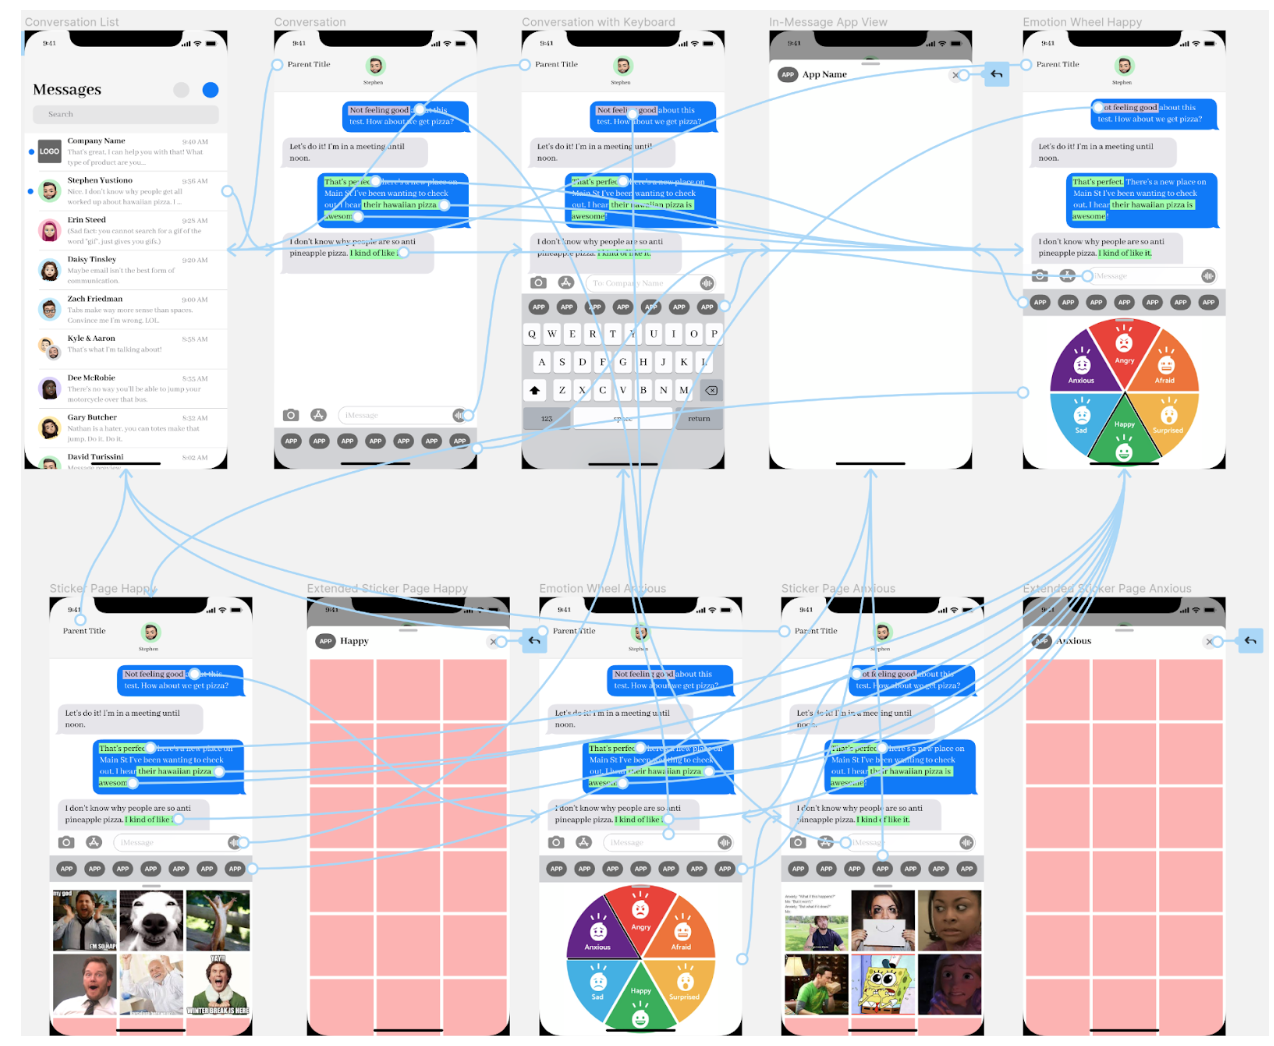
\includegraphics[width=1.0\linewidth]{figures/Figma_Prototype.png}
\caption{Figma Prototype with Interaction Arrows}
\label{fig:figmaprototype}
\Description{}
\end{center}
\end{figure}


\section{User Evaluation}
% Does "9 User Evaluation" section contain a proper summary of the purpose of the experiments, method, tasks and procedures, and participants? Does the method subsection indicate which user requirements the evaluation tested the designs against?
The final Prototype Evaluation aims to quantify the extent to which the functional high-fidelity prototype can fulfill the user requirements. It also checks if the prototype can provide a fluid flow of usage with minimal usability concerns or issues by the target users. Based on the feedback from target users, researchers can then reflect on their designs and make final edits and corrections, and finally run the large-scale production and final release of the product. Our evaluation targets the user requirements we mentioned above - users can easily access the emotional context of the messages and conveniently enhance the message with additional non-textual content (e.g., emoji, images, memes, etc). 


\subsection{Method}
We designed our experiment in a within-subject manner. Each participant is presented with two mobile messaging apps: iMessage and our app. We choose iMessage as a baseline due to its pervasive use by many users and its lack of emotion detection or features related to our system requirements. Thus, it can be a fitting baseline compared to our app, as our app is seeking to demonstrate superior emotion-supportive functions. After completing the tasks described below, we conduct a post-interview to understand what barriers the user encounters when navigating the app and if they have additional suggestions for us to improve the app. We also ask them to rank each of our unique features on a Likert scale of 1-5 (more details are provided in Task and Procedures) and provide the reasons behind each score they give. These Likert scores will be used for statistical analysis. We chose a standard alpha value of 0.05 for our statistical analysis.


\subsection{Apparatus}

As mentioned in Section \ref{sec:final_design}, we used Figma to design our prototype. Designs in Figma have a built in prototype mode that will model interactions between the various screens. We used this as our apparatus for user evaluation. Additionally, we used an iPhone to similarly model parallel iMessage functionality, which served as our baseline.


\subsection{Tasks and Procedures}
The main task we want our participants to accomplish is to navigate and compare the two given UIs, iMessage and our prototype. More specifically, we want the participants to first identify the tone/emotion from the previous messages. Then the participants need to find a meme that suits the identified emotional context and attach it to the chat. 

First, we inform our participants of the tasks to accomplish. Remind them that only de-identified information will be collected. We then also let them know they can quit at any time and that they are in no way obligated to complete the prototype evaluation, even if they start the evaluation. 

The researcher then informs the participant that they will be completing the tasks on the iMessage platform first. The researcher will use an Apple device and set up a conversation in advance to mirror the conversation in the Figma prototype. The researcher will instruct the participant to perform think-aloud (verbalize their thoughts while interacting with iMessage) and let them know you will be able to answer simple clarifying questions but nothing more until after the evaluation study is complete. Inform the participants that this task is designed to evaluate the following contexts: 

\begin{itemize}
    \item Upon navigation to a conversation page, users need convenient access to information about the emotional context and content from the previous messages.
    \item After composing a message, users need additional ways to enhance the textual content of a message (i.e., emoji, images, emotional indicators, etc.) in order to deliver their intent unambiguously.
\end{itemize}

The researcher hands the participant the Apple device. Tell the participant that if they wish to click on anything, verbally say “I am clicking on [whatever they are clicking on].” while performing the action. Likewise, if the user is swiping in any direction, they will verbally say “I am swiping left.” or “I am swiping up.”, etc. This will then give the interviewer the opportunity to record detailed interpretations.

\begin{enumerate}
    \item Instruct the participant to complete the two tasks in whatever order they wish, perhaps simultaneously.
    \item Record any difficulties users encountered, and any errors they made.
    \item Make sure the users are following the think-aloud protocol to provide their thoughts on each action they take.
    \item Once the task is completed, ask participants to give ratings for the following, and provide a brief description for each given score.
        \begin{itemize}
            \item Question 1: How difficult is it to identify the tone/emotion from the previous message? (1 being very easy, 5 being very difficult)
            \item Question 2: How difficult is it to find a meme online that suits the emotional context? (1 being very easy, 5 being very difficult)
            \item Question 3: Overall satisfaction while performing the task. (1 being very dissatisfied, 5 being very satisfied)
        \end{itemize}
\end{enumerate}

The researcher performs the same procedures (3) for the Figma prototype. Once the Final Prototype Evaluation is complete, indicate to the participant that the test is complete and thank the participant for their time.


\subsection{Participants}
%\instructions{Please provide demographic information of participants: number of participants, by age, by gender, by disability if relevant for the study, by experience with task, location, any other criteria for recruitment, how they were recruited, were they given any incentives, mode of study conducted (virtual or in-person) How was consent for participation sought and administered? How did you decide on the number of participants for your study?}
Our main inclusion criteria for this evaluation was familiarity with messaging apps and smartphone interfaces. This would allow for a shared background between participants, and potentially limit the learning curve for the messaging app in general and allow the participants to focus on the emotional context features that we are testing. 

We determined the number of participants (across the entire group) using GPower. We were looking for a medium effect size with statistically significant alpha and beta values, but not so large that it required an overly large sample size. We chose a Wilcoxon signed rank test for use on our paired Likert scale data, as we did not assume a normal distribution in our data. With two tails, an effect size of 0.5, a p-value of 0.05, and a beta of 0.8, GPower informed us that we needed a sample size of 23 participants. We have five people in our group, so we divided that evenly between each of us and recruited 5+ participants per group member. We ended up with 29 total participants.

Participant demographics information is attached in appendix \ref{final_pro_data}. We collected data from 29 participants. 

\subsection{Results}
\label{sec:user_eval_results}
% Does "9 User Evaluation" section contain results of statistical analysis of quantitative data? Does it contain proper interpretations of the statistical analysis?

Our data consisted of Likert scale ranking for three questions, compared between a control (iMessage interface) and our prototype (interface designed in Figma). The Wilcoxon signed rank test was the appropriate test for our data. Our null hypothesis for each of the three questions was that there is no difference between the responses for the control and for our prototype. The raw data is displayed in histograms in Figures \ref{fig:results1}, \ref{fig:results2}, and \ref{fig:results3}.

\begin{figure}[H]
\begin{center}
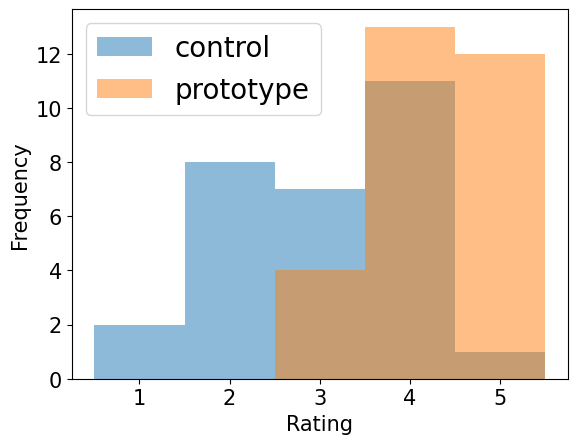
\includegraphics[width=0.6\linewidth]{figures/stats_resultsoutput.new.png}
\caption{Raw Response Data for Question 1 (Tone)}
\label{fig:results1}
\Description{}
\end{center}
\end{figure}

For the first survey question, most users think that our prototype does provide easy access to tone/emotion for previous messages, compared to iMessage. In contrast, most participants hold a neutral opinion on iMessage. 

\begin{figure}[H]
\begin{center}
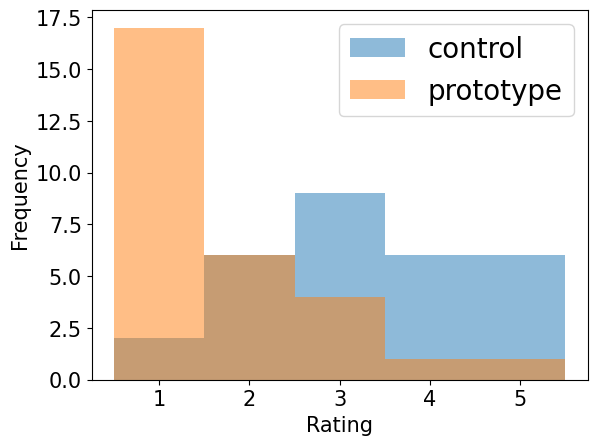
\includegraphics[width=0.6\linewidth]{figures/stats_resultsoutput2.new.png}
\caption{Raw Response Data for Question 2 (Meme)}
\label{fig:results2}
\Description{}
\end{center}
\end{figure}

For the second question, more than 80\% of our participants suggested that it is "very easy" or "easy" to find memes online that suits the emotional context using our prototype. Almost 70\% of our participants find it difficult using iMessage. 

\begin{figure}[H]
\begin{center}
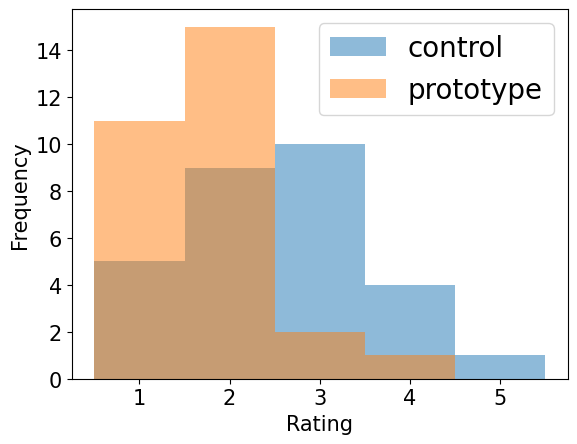
\includegraphics[width=0.6\linewidth]{figures/stats_resultsoutput3.new.png}
\caption{Raw Response Data for Question 3 (Satisfaction)}
\label{fig:results3}
\Description{}
\end{center}
\end{figure}

Lastly, for the third question, almost 100\% of our participants are "very satisfied" with the overall experience of playing with our prototype. On the other hand, the ratings for iMessage are more evenly distributed and have a long left tail. 

The results from the Wilcoxon signed rank test are in Table \ref{tab:stats_results}. As mentioned earlier, our alpha value was 0.05. Each of the tests had a p-value less than 0.05 for an effect size of 0.5, and therefore we reject the null hypothesis. There does appear to be a difference between the responses for the control and for our prototype. The ramifications of this result are further discussed in Sections \ref{sec:discussion} and \ref{sec:conclusion}.

\begin{table}[H]
\begin{tabular}{|l|l|l|l|}
\hline
Question & Control Mean & Prototype Mean & P-Value \\ \hline
1 & 2.55 & 1.76 & 0.000295 \\ \hline
2 & 3.28 & 1.72 & 0.000149 \\ \hline
3 & 3.03 & 4.28 & 0.000144 \\ \hline

\end{tabular}
\caption{Wilcoxon signed rank test results - Control vs Prototype}
\label{tab:stats_results}
\end{table}

The anonymized and de-identified participants data is attached on appendix \ref{final_pro_data}. 


\section{Discussion}
\label{sec:discussion}
%\instructions{You will keep updating this section after each assignment. After each assignment you will add discussion about what the results mean for your research.}
The context of use survey helped us to refine our focus from a general purpose sentiment analysis tool for all contexts, to a sentiment analysis tool that focuses on conveying the appropriate tone in a non-professional context. This shift in focus is supporting by the following paragraphs discussing our survey results.

For difficulty expressing oneself and severity of misunderstandings, it may be that the average audience of an email or social media post is larger than the average audience of a text, and this increases the difficulty of expressing oneself as well as the severity of misunderstandings. Future qualitative data should be collected to accept or reject this hypothesis. 

Phone calls were universally easier to understand than text, email, or social media, and video chats were even easier than phone calls. This suggests that the facial and body language aspect of a video call gives a concrete advantage over just voice on a phone call. This may have implications for the use of emojis or other visually expressive mediums when improving text entry on text, email, or social media.

Qualitatively, the participants largely referenced texting when narrating misunderstandings with substantial consequences. Future work could further differentiate between the frequency and severity of misunderstandings. 

There was a notable difference between the rankings of clarity, concision, accuracy, and tone between professional and non-professional settings. This suggests that clarity and accuracy are equally weighted and valued in all contexts, with concision being less important than both; however, tone oscillates between extremely important and not important at all depending on the context, audience, and perhaps the medium of communication as well.

Our participants widely use auto-correct and generally express satisfaction with the results. Interestingly, they indicate that typos do not significantly hinder their communication; our survey design makes it unclear whether this is true in general, or whether auto-correct is a causal mechanism.

"Changing text without confirmation" was overwhelmingly the most irritating feature of auto-correct for our participants, with over 90\% indicating this option. However, 20.8\% of participants indicated that "changing text without confirmation" was a feature they enjoyed. This suggests an intersection between the two answer choices, describing a population that enjoys the feature despite being irritated with its current implementations. This may have other connections with the participants who enjoy a list of options when using auto-correct.

The question about which software tools participants use to improve text may have unreliable results, and therefore may affect the results of following questions. While the literature on default settings on mobile phones is incomplete, current knowledge suggests a significant majority of smartphone users keep most or all of the default settings on their phones. The fact that nearly all participants used a cell phone in the past week, but only a tiny minority indicated that they use their phone's default auto-correct raises questions. It may be that participants use software tools to improve text without realizing they are using them, or survey fatigue may have led participants to give less complete answers to this last section of questions.

While our initial survey established understanding emotional context as a broad focus, the contextual interviews deepened our understanding of the nuances of this focus. The most important breakdowns within this focus ended up happening during an incoming message and while drafting a response. Interventions at either one of these two stages could have mitigating effects on misunderstandings.

Additionally, our initial focus was centered on simply understanding the tone of a message. The contextual interviews broadened our focus to include improving upon an existing message draft where the tone may be poorly communicated. This is supported by the explanation in the third user requirement in Table \ref{tab:user_requirement}.

Upon the isolation (and further revision of) the user requirements for this research focus, the design phase resulted in a number of distinct designs, each with their own strengths and weaknesses.

Among the common features included in the designs were, unsurprisingly, both emotional cues for incoming and outgoing messages, and a content-aware refreshers for conversations. One distinction among the designs were the particular implementations of the feedback (emoji, text, highlighting), and the modality (integrated vs. web-based). Key themes that emerges from our design critiques included the need for feedback for both incoming and outgoing messages, as well as key issues about the discoverability and significance of different parts of the designs. Some designs included features that were not easily discoverable, or where it wasn't apparent what would happen if a participant used a certain feature. 

Usability evaluation is an essential part of the user-centered design process. It helps designers optimize usability and remove or minimize any design deficiencies. Through demoing our low-fidelity prototype, usability experts were able to identify many usability issues and design flaws as shown in the previous sections. All 5 usability experts pointed out that our design is not consistent and it does not follow standards. The team needed to come up with a more conventional way to display the detected tones while still being differentiable to signals from the built-in auto-correct.

Simplified user testing gives designers the opportunity to bring their designs to actual users, and test if their solutions can satisfy user requirements. Most of the participants were overwhelmed by the dense coloring and were confused about the color-tone mapping, and this issue is also discerned by our usability experts. This led to a primary focus of better visualization for tones during the final prototype design. In addition, both many experts and users mentioned that labeling phrases or words are unnecessary. Instead, having an overall tone for a message would be more user-friendly. This seems to connect with our initial survey results that indicate frustration from users with existing auto-correct tools. It may be the granularity of existing tools is too great, and our paper prototype also had too fine of granularity, and our users requested more coarse tools as a result.

The final prototype incorporated feedback from all of the design stages. The means for all three questions showed a more positive rating for our prototype versus the control, and this result was statistically significant, as demonstrated in Section \ref{sec:user_eval_results}. One interesting point is that the effect was so large. It may be that users reacted more to a lack of emotion-based tools in iMessage than they specifically preferred the exact layout of our tools. In other words, something is better than nothing. In this sense, the most important takeaway from this statistical analysis is that users want integrated emotion-based tools in their digital communications, and future iterations of our tools may be much more effective than the final prototype design presented in this paper. However, it is still important to consider that using the Likert scale, while a quantitative metric, is still a qualitative way for the user to subjectively rank the design.

\section{Conclusion and Future Work}
\label{sec:conclusion}
%\instructions{What is the takeway of this project? Were there any parts of the project that you did not include in the scope of this project? Here is where you will discuss how the current assignment will inform the rest of your project. For example, in Assignment 1, how will the results of your survey influence the future steps in understanding context of use? Feel free to use your creativity to suggest new research directions, designs---but these suggestions must be supported by the findings of your study}

\subsection{General Takeaways}
% Overall, the results show a fairly accurate representation of the population in regards to gender split. The age split and level of education, however, is biased. This can be explained because the research group is composed of graduate students, and the easiest available population for us to survey are also younger individuals with at least a Bachelor's Degree.

Participants expressed particular difficulty in preventing misunderstandings in textual mediums as opposed to audio-visual mediums. Auto-correct systems are widely used and appreciated, but certain features can unintentionally impede communication, like replacing content without user confirmation. Furthermore, auto-correct lacks the sophisticated context and tonal features that users appreciate in the popular tool Grammarly.

It is also notable that when people are worried about a digital message, many prefer consulting another person rather than using a digital assistant or tool. Available software may be oriented towards professional contexts and tend to misinterpret informal messages. 

The proposed tool is one that provides an emotional context for existing conversations through text highlighting or emoji provision and gives emotional immediate feedback after the drafting of a message to ensure clear communication and tonal coherence. 

The initial design stages provide insightful information about what the proposed tool should look like. Even with the same set of user requirements, each individual design was tailored toward different target audiences (personas); resulting in various user interfaces and functions. The team then came together, criticized each design, and developed the final sketch, storyboard, and paper prototype. 

During this process, the team identified ambiguity within the user requirements which were specified at the earlier stage. The team realized it is necessary to analyze the recorded interpretations from contextual inquiry very carefully. The number of scenarios should be reduced, and each scenario should be grounded in the context of use. A breakdown we encountered is that the number of interpretations we had was overwhelming and many of them were difficult to be categorized. This affects the development of user requirements, which ultimately influence design choices. Furthermore, the user requirements need to be further consolidated, ensuring that they are objective, testable, comprehensive, and grounded in the context of use. 

Through the heuristic evaluation with five experts, the team identified several issues not found when drafting the app prototype. The team discussed and came up with several points to improve the next iterations of the prototype and create high-fidelity functionalities. For instance, as reported severe problems in \emph{Recognition and Recall}, we should devise the highlighted color and invent alternatives to make them more easily identified and interpreted by users. Issues found in Aesthetic and Minimalist Design also reflected the usability problems in highlighted colors in that they distract the users and are intrusive during usage. Our app should value these insightful suggestions and correct the identified issues to make our app more usable and user-friendly. 

Through the simplified user testing, the team also understood the mental model and the interpretations of the general users towards our app prototype. The team identified and synthesized the difficulties the participants encountered and the confusion the participants brought up. We realized that the app should not be only designed by ourselves or based on our own experience, but rather, we should testify our ideas with real users. By doing so, we can understand how potential bias we had with the users, and possibly, we can involve users in every design stage in future work, which would be a participatory design approach or user-centered design approach to ground our design choices more tangibly.

The final prototype was positively received across the testing population. As mentioned in the discussion, this seems to be a referendum on the saturation of grammatical and syntactical tools embedded in iMessage, and the corresponding lack of tools related to the emotional content of messages. 

\subsection{Shifting Focus}
The primary research questions of this project were the following:
\begin{enumerate}
  \item Where do miscommunications occur?
  \item How do people combat miscommunications?
  \item Are existing tools satisfactory?
\end{enumerate}

%After the completion of the survey, it appears that there is a lack of tools for non-professional contexts to help with tone and misunderstandings. Many existing tools, like Grammarly and auto-correct, that can assist with formal writing. However, there is not a common and easy to use tool that helps with writings in non-professional contexts. Auto-correct often misunderstands social queues and contexts and can often cause more problems than it fixes. Thus, our scope will shift towards tools that can help improve with more informal, non-professional writing.

Upon analysis of survey, the most promising focus moving forward is a tonally aware analysis tool for personal communication. This is due to the participants' appreciation of the nuanced understanding of Grammarly, participants' emphasis on the importance of tone in non-professional communication, and some user stories which present examples of miscommunication.

The design and prototyping process reaffirms this shift in focus and highlights a persona, Monica, in her non-professional communication.

\subsection{Future Directions}
The survey results have shown insights into the current state of text entry. For professional writing, people rely on "heavy" tools. In this case, people tend to spend more time revising their texts. Tools like Grammarly satisfied most of their needs. For informal/non-professional communication people rely on built-in text assistant tools like auto-correct. It functions in real-time and makes adjustments or suggestions while typing, which made it well suited for casual conversations where the turn-around time is relatively short. However, it only provides word-based feedback. This allows it to capture misspellings very well, but it ignores contextual information, often misinterpreting a user's intention. There is no existing tool that is not as cumbersome as professional software but provides better sentiment feedback than auto-correct. In addition to basic spelling and grammar check, the team envisions this tool to have simple contextual understanding for short messages. This tool may providing real-time suggestions about tone, tense, and semantics to limit not only mistyping but also misunderstandings. 

% In terms of potential project ideas, it is looking like we will be developing a tool that will be able to efficiently and promptly streamline informal writing that helps with using appropriate tone in informal/non-professional conversations. 

It can potentially be integrated into auto-correct or it could be stand-alone tool parallel to auto-correct.

Through heuristic evaluation and simplified user testing, we identified key usability issues and improved our app aesthetics to make the functionalities more recognizable and user-friendly. Continued iterations on this process would be beneficial in more fully meeting the user requirements. Additionally, our final prototype was focused on the UI/UX implementation. A backend implementation that uses NLP or similar technology could allow for development of an end-to-end tool that fully demonstrates our design and could be tested more widely.

Our statistical analysis was focused on a baseline of the iMessage platform. iMessage is one of the most popular global messaging applications, so we believe the conclusions are generalizable. To confirm this, future studies could evaluate whether the effect is maintained across different platforms that have different embedded tools within their chat applications. 

% Upon the creation of the paper prototype, future work will consist of the user testing by doing "Wizard of Oz" of our paper prototype with 3-5 potential users. Following this, further iterations of the prototype can be implemented and similarly tested.

% However, since more people use laptops and phones, it is most likely we will pursue an option that utilizes one or both of these hardware types. 

% While we are still brainstorming ideas for the project, we will keep in mind the context of use results we collected here and may potentially revisit surveying in the future if our vision loses focus.


%%
%% The acknowledgments section is defined using the "acks" environment
%% (and NOT an unnumbered section). This ensures the proper
%% identification of the section in the article metadata, and the
%% consistent spelling of the heading.
\begin{acks}
%\instructions{Here, you will acknowledge any individuals or organizations that are not part of your group, but that have contributed to your work.}
We would like to acknowledge the teachings and guidance of Nikola Banovic, the instructor for the University of Michigan Fall 2022 EECS 593 course.
\end{acks}

%%
%% The next two lines define the bibliography style to be used, and
%% the bibliography file.
\bibliographystyle{ACM-Reference-Format}
\bibliography{base}

%%
%% If your work has an appendix, this is the place to put it.
\appendix

\section{Responsible Research: Human Subjects Research Protections}
%\instructions{This is where you will include PEERRS Human Subjects Research Protections certification for each of your group members. You can download your certification as a PDF and use one figure per group member to include the PDFs in this appendix section.}

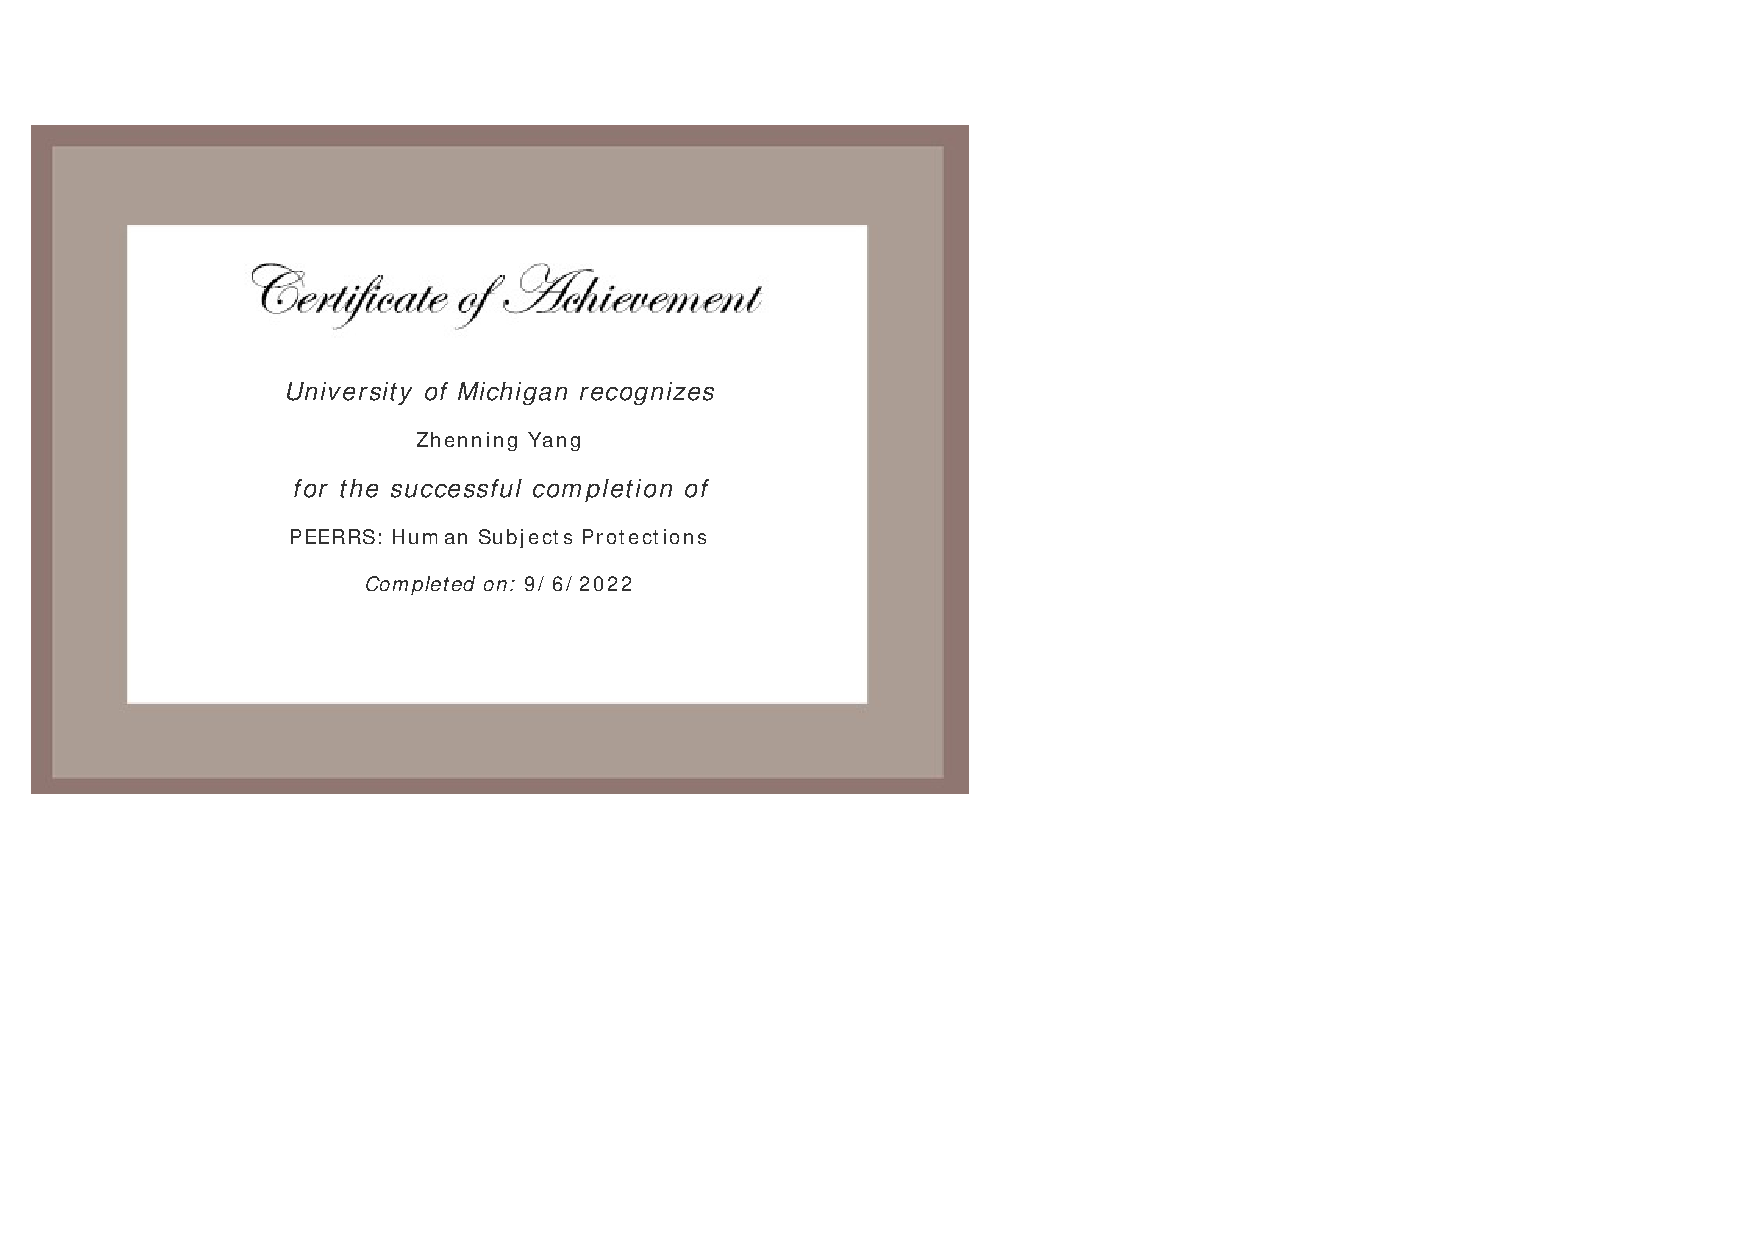
\includegraphics[width=1.0\linewidth]{ {./PEERRS_certs/zy_cert.pdf} }

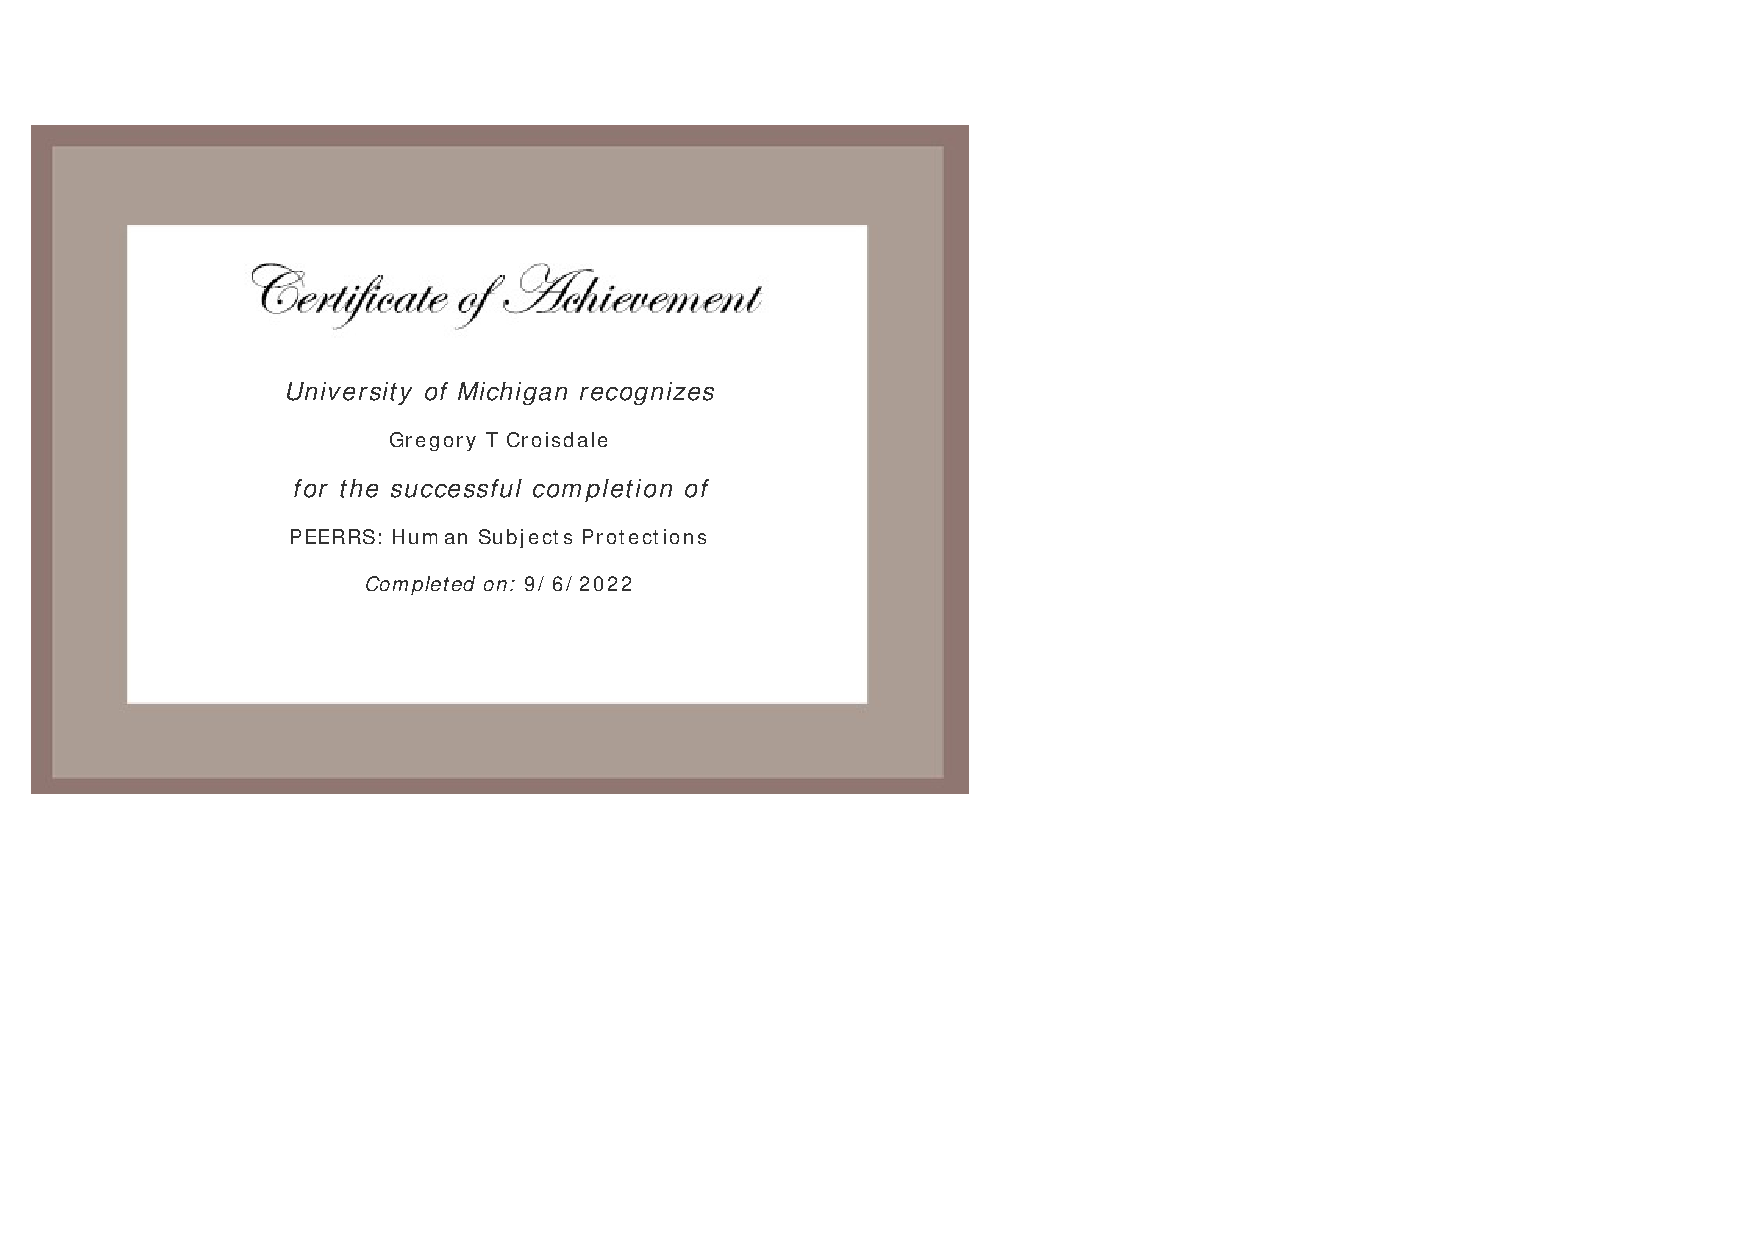
\includegraphics[width=1.0\linewidth]{ {./PEERRS_certs/gc_cert.pdf} }


\includegraphics[width=1.0\linewidth]{ {./PEERRS_certs/rc_cert.pdf} }

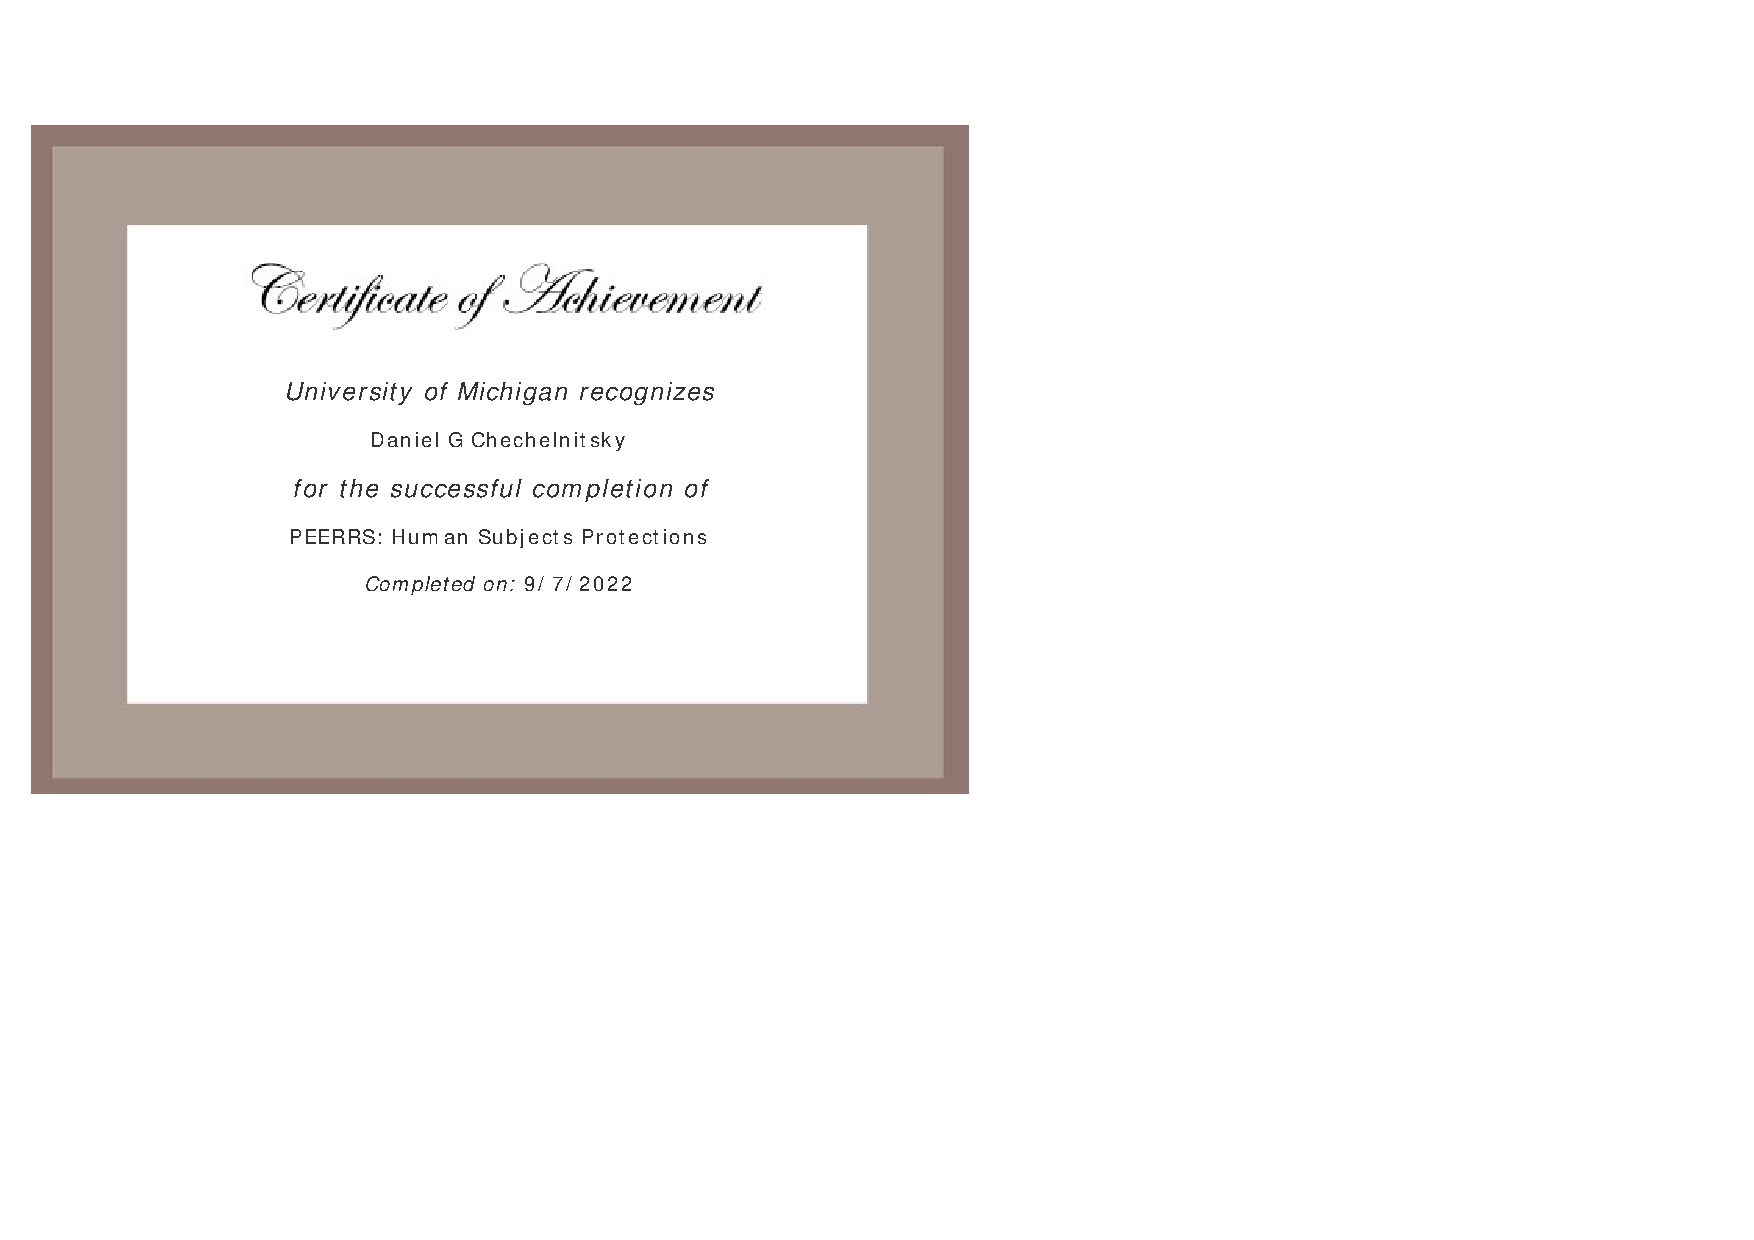
\includegraphics[width=1.0\linewidth]{ {./PEERRS_certs/dc_cert.pdf} }

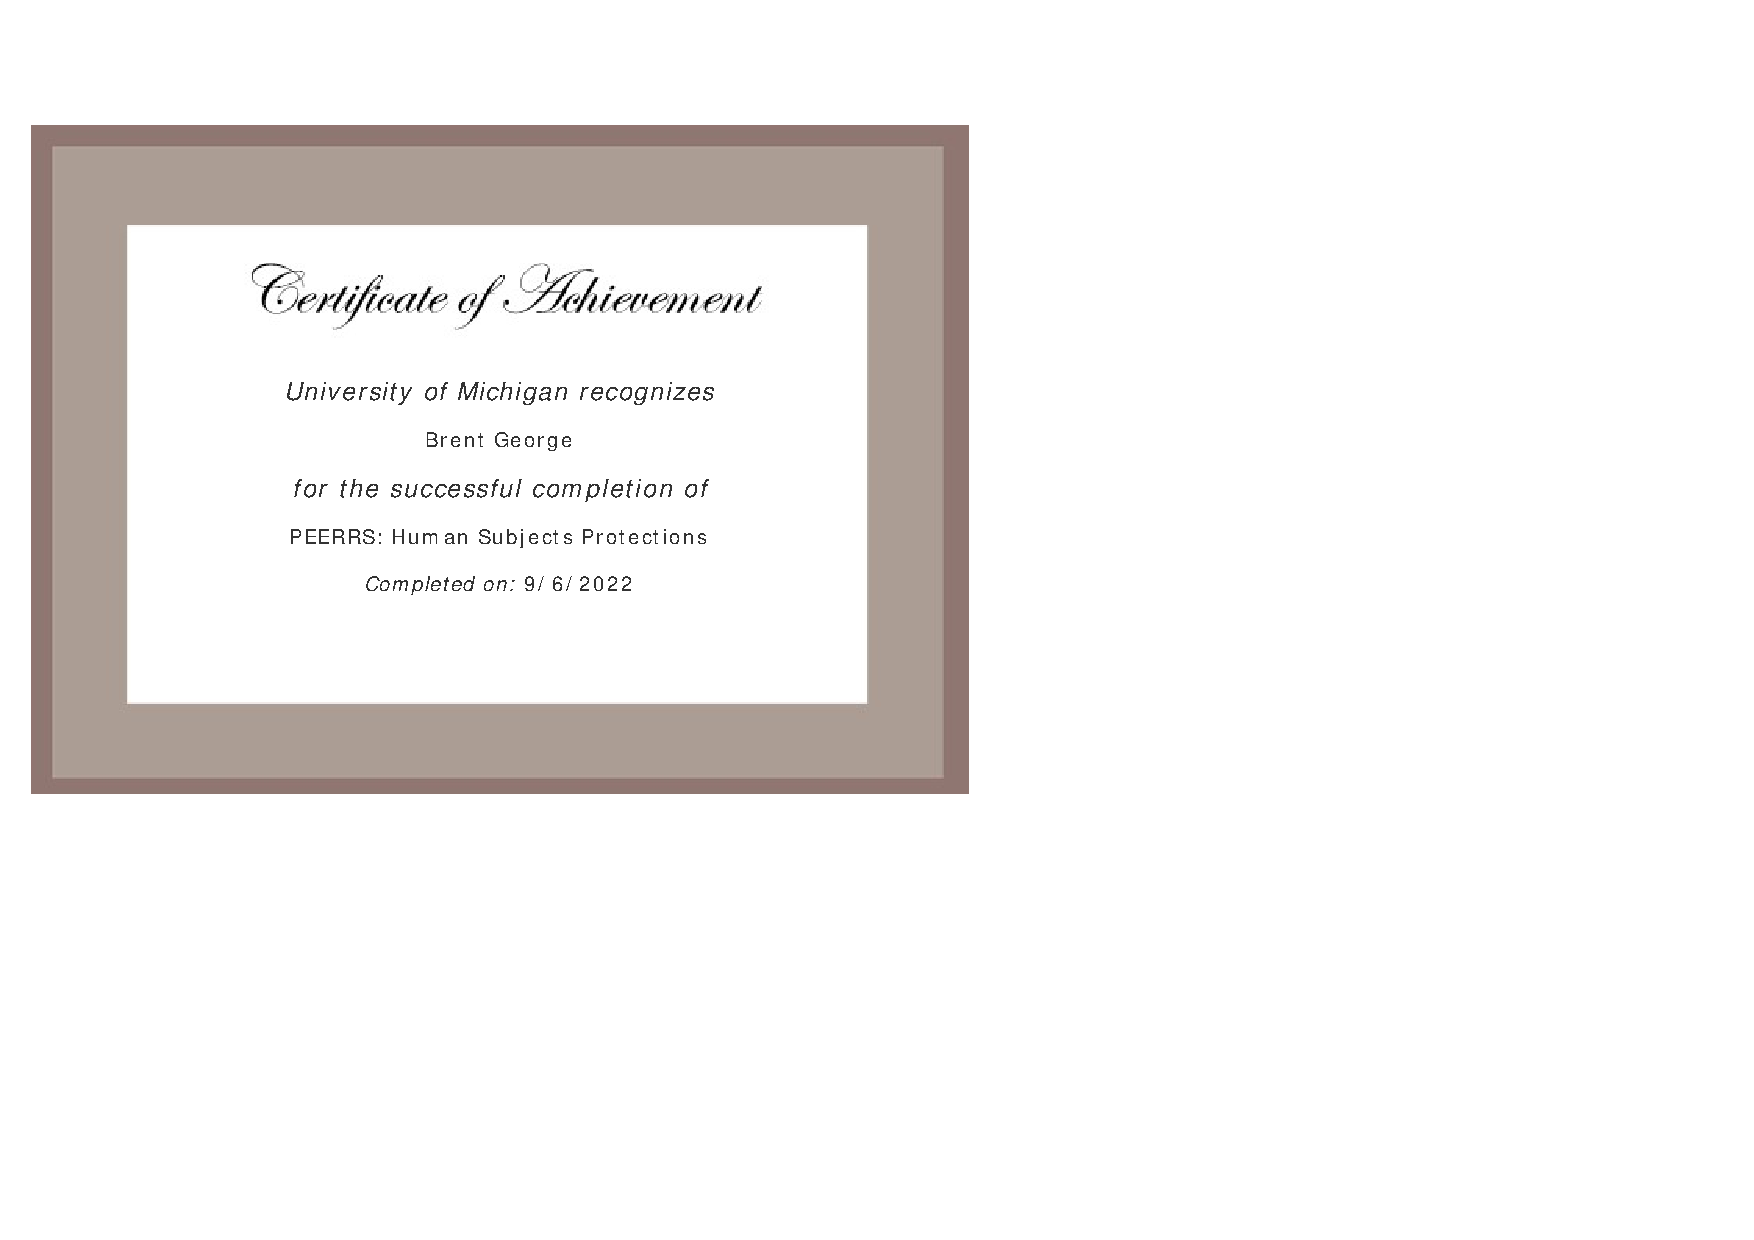
\includegraphics[width=1.0\linewidth]{ {./PEERRS_certs/bg_cert.pdf} }
  

\section{Survey and Questionnaire Instruments}
%\instructions{This is where all of your materials that you created for Assignment 1 go.}

\subsection{Initial Questionnaire Design}
\label{initial_Questionnaire_Design}

% \TODO{Add all 5 surveys here}

% % Matches the order in Sec 3, pilot run
% 1. Brent's initial survey
% 2. ZY's initial survey
% 3. Ruei-che's initial survey
% 4. Daniel's initial survey
% 5. Greg's initial survey

% 1. Brent's initial survey
\subsubsection{Variant \#1}
\label{var1}

Brent George's Initial Survey

\textbf{General Information}
\begin{enumerate}
    \item What is your gender?
        \begin{enumerate}
            \item Female
            \item Male
            \item Non-binary
            \item Other (specify)
        \end{enumerate}
    \item What is your age range?
        \begin{enumerate}
            \item Under 18
            \item 18-22
            \item 23-30
            \item 31-40
            \item 41-50
            \item 50 and over
        \end{enumerate}
    \item How many languages do you speak fluently?
    \item What is your highest level of education completed?
        \begin{enumerate}
            \item Some or no high school
            \item High School Diploma
            \item Bachelor's Degree
            \item Graduate degree
            \item Vocational/Technical school
            \item Other (specify)
        \end{enumerate}
    \item What devices do you use? (Multi-select)
        \begin{enumerate}
            \item iPhone
            \item Samsung mobile phone
            \item Google mobile phone
            \item Other mobile phone
            \item Windows
            \item Mac
            \item Linux
            \item Tablet
        \end{enumerate}
        \item What social media platforms do you use? (Multi-select)
            \begin{enumerate}
                \item Twitter
                \item Instagram
                \item Facebook
                \item LinkedIn
                \item Tiktok
                \item Snapchat
                \item Other:
            \end{enumerate}
\end{enumerate}
\textbf{Misunderstanding}

 I will ask questions about various common digital experiences: sending texts, writing emails, making social media posts, and any other situations if you desire to specify.

\begin{enumerate}
  \item How difficult is it to express yourself on a scale of 1 to 5, with 1 being not difficult at all, and 5 being extremely difficult
  \begin{enumerate}
      \item Sending texts
      \item Writing emails
      \item Making social media posts
      \item Other (specify)
  \end{enumerate}
    \item How easy is it to be misunderstood on a scale of 1 to 5, with 1 being easily understandable, and 5 being very easily misunderstood
  \begin{enumerate}
      \item Sending texts
      \item Writing emails
      \item Making social media posts
      \item Other (specify)
  \end{enumerate}
  \item How often are you misunderstood, regardless of severity of the misunderstanding on a scale of 1 to 5, with 1 being not often, and 5 being very often
  \begin{enumerate}
      \item Sending texts
      \item Writing emails
      \item Making social media posts
      \item Other (specify)
  \end{enumerate}
  \item How severe are misunderstandings in the following formats, on a scale of 1 to 5, with 1 not severe, and 5 being very severe
  \begin{enumerate}
      \item Sending texts
      \item Writing emails
      \item Making social media posts
      \item Other (specify)
  \end{enumerate}
  \item What methods do you employ when you are worried about the clarity of a message?
  \begin{enumerate}
      \item Ask another person
      \item Use a software tool (Grammarly, etc.)
      \item Revisiting a message in the moment (rereading, revising, etc)
      \item Revisiting a message at a \underline{later time} before sending
      \item Refraining from sending any message
      \item Other (specify)
  \end{enumerate}
  \item In which ways do you wish you could improve your communication style when sending texts, writing emails, making social media posts?
  \begin{enumerate}
      \item Clarity
      \item Concision
      \item Appropriate Tone
      \item Respect
      \item Other (specify)
  \end{enumerate}

\end{enumerate}

\textbf{Mistypings / Typos}
\begin{enumerate}
    \item How often do you mistype? (split out per device and language as answered above) scale of 1 to 5, 1 being not often and 5 being very often, n/a meaning you do not type in this language
    \item What are common causes of mistyping?
    \begin{enumerate}
        \item Layout of letters on keyboard
        \item Keys too small
        \item Difficult sequencing of letters in a word you are trying to spell
        \item Other (specify)
    \end{enumerate}
\end{enumerate}


% 2. ZY's initial survey
\subsubsection{Variant \#2}
\label{var2}

Zhenning Yang's Initial Survey

\textbf{General Information}
\begin{enumerate}
    \item What is your gender?
        \begin{enumerate}
            \item Female
            \item Male
            \item Other
        \end{enumerate}
    \item What is your age range?
        \begin{enumerate}
            \item Under 18
            \item 18-22
            \item 23-30
            \item 31-40
            \item 41-50
            \item 50 and over
        \end{enumerate}
    \item How many languages do you speak?
    \item What is your education level?
        \begin{enumerate}
            \item High School Diploma
            \item Bachelor's Degree
            \item Advanced Degree (Master's Degree, Ph.D. etc)
            \item Other
        \end{enumerate}
    \item Do you enter text mostly with?  (Multi-select)
        \begin{enumerate}
            \item Virtual keyboards
            \item Handwriting recognition
            \item Voice recognition
            \item Laptop keyboards
            \item Desktop keyboards
        \end{enumerate}
        \item What social media platforms do you use? (Multi-select)
            \begin{enumerate}
                \item Twitter
                \item Instagram
                \item Facebook
                \item Other:
            \end{enumerate}
\end{enumerate}
\textbf{Misunderstanding}
\begin{enumerate}
    \item In which contexts do you find it difficult to express yourself? (Give a brief description after the selected option)
        \begin{enumerate}
            \item Sending texts
            \item Writing emails
            \item Making social media posts
            \item Designing surveys
            \item Others: 
        \end{enumerate}
    \item What methods do you employ when you are worried about the clarity of a message?
        \begin{enumerate}
            \item Ask a colleague
            \item Use a software tool (Grammarly, etc.)
            \item Revisiting a message later
            \item Others:
        \end{enumerate}
    \item In which ways do you wish you could improve your communication style?
        \begin{enumerate}
            \item Clarity
            \item Concision
            \item Others:
        \end{enumerate}
    \item If you were to design a tool to help; what features would you add? And how does it function?
\end{enumerate}

\textbf{Mistypings / Typos}
\begin{enumerate}
    \item In what situations have you found yourself mistyping more often than usual?
    \item What do you think causes this?
    \item Do you use the built-in auto-correct feature? If yes, what are your opinions on this feature?
\end{enumerate}

\textbf{Tools}
\begin{enumerate}
    \item How often do you use external apps or websites like Grammarly, Google translate, etc?
        \begin{enumerate}
            \item Never 
            \item Rarely
            \item Sometimes
            \item Always 
            \item Often
        \end{enumerate}
    \item If you have never used them, briefly describe the reason. If you have used them, briefly share your thoughts.
    \item If you could change one thing about the current text entry interface or device, what would it be?
\end{enumerate}

\subsubsection{Variant \#3}
\label{var3}

Ruei-che Chang’s Initial Survey

\textbf{General Information}
\begin{enumerate}
    \item What is your gender?
        \begin{enumerate}
            \item Female
            \item Male
            \item Other
        \end{enumerate}
    \item What is your age range?
        \begin{enumerate}
            \item Under 18
            \item 18-22
            \item 23-30
            \item 31-40
            \item 41-50
            \item 50 and over
        \end{enumerate}
    \item What is your education level?
        \begin{enumerate}
            \item High School Diploma
            \item Bachelor's Degree
            \item Advanced Degree (Master's Degree, Ph.D. etc)
            \item Other
        \end{enumerate}
    \item What is your common text-entry method? 
        \begin{enumerate}
            \item Keyboard
            \item Speech input
            \item Gesture type
            \item Shortcut
            \item Handwriting
            \item Other
        \end{enumerate}
        \item What devices do you use?  (Multi-select)
            \begin{enumerate}
                \item iPhone
                \item Samsung
                \item Google Pixel
                \item Laptop / Desktop
                \item Other:
            \end{enumerate}
        \item What social media platforms do you use? 
            \begin{enumerate}
                \item Twitter
                \item Instagram
                \item Facebook
                \item Other
            \end{enumerate}
        \item What languages of keyboard do you use?
            \begin{enumerate}
                \item English
                \item China (pinyin)
                \item China (Mandarin)
                \item Indian
                \item French
                \item Japan
                \item Thailand
                \item Korean
                \item Germany
                \item Brazil
                \item Egypt, Saudi Arab, Arab Emirates
                \item Colombia, Mexico
                \item Spain
                \item Indonesia
                \item Iran
                \item Italy
                \item Nigeria
                \item Russia
                \item Viet Nam
                \item Turkey
                \item Other
            \end{enumerate}
\end{enumerate}

\textbf{Misunderstanding}
\begin{enumerate}
        \item In which contexts do you find it difficult to express yourself? (Give a brief description after the selected option)
            \begin{enumerate}
                \item Sending texts
                \item Writing emails
                \item Making social media posts
                \item Designing surveys
                \item Communicating research ideas/projects
                \item Casual chat with friends
                \item Others: 
            \end{enumerate}
        \item What methods do you employ when you are worried about the clarity of a message?
            \begin{enumerate}
                \item Ask a colleague
                \item Use a software tool (Grammarly, etc.)
                \item Revisiting a message later
                \item Use Emoji/GIFs to support
                \item Others: 
            \end{enumerate}
        \item (Following the previous question) Why do you employ these methods? Please briefly answer.
\end{enumerate}

\subsubsection{Variant \#4}
\label{var4}
Daniel Chechelnitsky’s Initial Survey 

\textbf{General Information}
\begin{enumerate}
    \item Please enter your gender below:
        \begin{enumerate}
            \item Fill in the blank
        \end{enumerate}
    \item Please select the age range you are in.
        \begin{enumerate}
            \item <17
            \item 18-22
            \item 23-30
            \item 31-40
            \item 41-50
            \item 51+
        \end{enumerate}
    \item How many languages do you speak? Enter below:
        \begin{enumerate}
            \item Fill in the blank
        \end{enumerate}
    \item Please select your highest level of education.
        \begin{enumerate}
            \item Undergrad
            \item Some grad
            \item Grad
            \item Other (enter here):
        \end{enumerate}
    \item What devices do you use? Select all that apply.
        \begin{enumerate}
            \item iPhone
            \item Samsung
            \item Google Pixel
            \item Laptop / Desktop
            \item Smart Watch
            \item Other (enter here):
        \end{enumerate}
        \item What social media apps do you use (tools within the apps)? Select all that apply.
            \begin{enumerate}
                \item Twitter
                \item Instagram
                \item Facebook
                \item Other (enter here):
            \end{enumerate}
\end{enumerate}
\textbf{Misunderstanding}
\begin{enumerate}
    \item In which contexts do you find it difficult to express yourself/say what you mean? Select all that apply.
        \begin{enumerate}
            \item Sending texts
            \item Writing emails
            \item Making social media posts
            \item Designing surveys
            \item Other (enter here):
        \end{enumerate}
    \item What methods do you employ when you are worried about the clarity of a message? Select all that apply.
        \begin{enumerate}
            \item Ask a colleague
            \item Use a software tool (Grammarly, etc.)
            \item Revisiting a message later
            \item Other (enter here):
        \end{enumerate}
    \item In which ways do you wish you could improve your communication style? Select all that apply.
        \begin{enumerate}
            \item Clarity
            \item Concision
            \item Politeness
            \item Other (enter here):
        \end{enumerate}
\end{enumerate}

\textbf{Mistypings}
\begin{enumerate}
    \item How often do you mistype?
        \begin{enumerate}
            \item Never
            \item Once a week
            \item Once a day
            \item Multiple times a day
        \end{enumerate}
    \item What do you think causes this? Select all that apply.
        \begin{enumerate}
            \item Language barrier
            \item Keyboard too small/big
            \item Spelling challenges
            \item Other (enter here):
        \end{enumerate}

\end{enumerate}

\textbf{Tools}
\begin{enumerate}
    \item Opinions on existing tools (like Grammarly, auto-correct, or even hardware design, etc)?
        \begin{enumerate}
            \item Good (or more positively leaning)
            \item Neutral
            \item Bad (or more negatively leaning)
            \item Haven’t used such tools.
        \end{enumerate}
    \item If you use such tools, what do you like about them?
        \begin{enumerate}
            \item Appearance
            \item Functionality
            \item Portability
            \item Other (enter here):
        \end{enumerate}
    \item If you use such tools, what do you think could be improved about them?
        \begin{enumerate}
            \item Appearance
            \item Functionality
            \item Portability
            \item Other (enter here):
        \end{enumerate}
\end{enumerate}

\subsubsection{Variant \#5}
\label{var5}
Gregory Croisdale's Initial Survey 

\textbf{General Information}
\begin{enumerate}
    \item What is your gender?
        \begin{enumerate}
            \item Fill in the blank
        \end{enumerate}
    \item What is your age range?
        \begin{enumerate}
            \item <17
            \item 18-22
            \item 23-30
            \item 31-40
            \item 41-50
            \item 51 up
        \end{enumerate}
    \item In which languages would you consider yourself to be conversational?
        \begin{enumerate}
            \item Fill in the blank
        \end{enumerate}
    \item What is your education level?
        \begin{enumerate}
            \item Some high school
            \item High school diploma
            \item Some undergrad
            \item Undergrad degree
            \item Some grad
            \item Graduate degree
        \end{enumerate}
    \item What devices do you use? (multi-select)
        \begin{enumerate}
            \item iPhone
            \item Samsung
            \item Google Pixel
            \item Laptop / Desktop
            \item Smart Watch
            \item Other
        \end{enumerate}
        \item What social media platforms do you use? (Multi-select)
            \begin{enumerate}
                \item Twitter
                \item Instagram
                \item Facebook
                \item Other
            \end{enumerate}
\end{enumerate}
\textbf{Misunderstanding}
\begin{enumerate}
    \item In a professional context, rank the following in order of importance
        \begin{enumerate}
            \item Clarity
            \item Efficiency / Concision
            \item Accuracy
            \item Tone
        \end{enumerate}
    \item In a social context, rank the following in order of importance
        \begin{enumerate}
            \item Clarity
            \item Efficiency / Concision
            \item Accuracy
            \item Tone
        \end{enumerate}
    \item Rank the following in order from highest difficulty communicating to lowest difficulty communicating
        \begin{enumerate}
            \item Sending texts
            \item Writing emails
            \item Making social media posts
            \item Professional writing (i.e., writing a paper, designing a survey, etc.)
        \end{enumerate}
    \item What methods do you employ when you are worried about the quality of a message?
        \begin{enumerate}
            \item Sending texts
            \item Writing emails
            \item Making social media posts
            \item Professional writing (i.e., writing a paper, designing a survey, etc.)
        \end{enumerate}
    \item In which ways do you wish you could improve your communication style?
        \begin{enumerate}
            \item Clarity
            \item Efficiency / Concision
            \item Accuracy
            \item Tone
        \end{enumerate}
\end{enumerate}

\textbf{Tools}
\begin{enumerate}
    \item Do you use Grammarly or other software tools to edit text?
        \begin{enumerate}
            \item Yes, Grammarly
            \item Yes, other
            \item No
        \end{enumerate}
    \item If previous, what features do you like?
        \begin{enumerate}
            \item (fill in blank)
        \end{enumerate}
    \item If previous, what features could be improved?
        \begin{enumerate}
            \item (fill in blank)
        \end{enumerate}
\end{enumerate}

\textbf{Mistypings}
\begin{enumerate}
    \item To what extent do mistypings impede your communication
        \begin{enumerate}
            \item Regularly impede
            \item Occasionally impede
            \item Rarely impede
            \item Never impede
        \end{enumerate}
\end{enumerate}

\subsection{Final Questionnaire Design}
\label{final_Questionnaire_Design}
\textbf{Misunderstanding}
\begin{enumerate}
    \item How difficult is it to express yourself and be understood properly in the following formats, on a scale of 1 to 5? (1 is not difficult at all, 5 is very difficult)
    \item How damaging is the average misunderstanding in the following formats, on a scale of 1 to 5? (1 is harmless, 5 is very harmful)
    \item What do you do when you are worried about a digital message (text, email, social media post) being misunderstood by the recipient(s)? 
        \begin{enumerate}
            \item Consult another person
            \item Use a software tool (Grammarly, etc)
            \item Revisit a message in the moment (rereading, revising, etc)
            \item Revisit a message at a later time before sending
            \item Choose not to send the message
            \item Other
        \end{enumerate}
    \item Rank the following goals from 1-4, in a \textbf{non-professional} context (for example, communicating with a friend or family member):
        \begin{enumerate}
            \item Clarity (how easy a message is to understand)
            \item Efficiency/Concision (message has appropriate focus and not too wordy)
            \item Accuracy (how much the information reflects reality)
            \item Tone (the mood of the message - friendly, serious, etc.)
        \end{enumerate}
    \item Rank the following goals from 1-4, in a \textbf{professional} context (for example, writing a business email or a paper):
        \begin{enumerate}
            \item Clarity (how easy a message is to understand)
            \item Efficiency/Concision (message has appropriate focus and not too wordy)
            \item Accuracy (how much the information reflects reality)
            \item Tone (the mood of the message - friendly, serious, etc.)
        \end{enumerate}
    \item (Optional) In which context do you find misunderstandings to be the most common? 
    \item (Optional) Is there a particular time a message you wrote was misunderstood and there were substantial consequences?
    \item (Optional) Is there a particular time you misunderstood a message and there were substantial consequences?
\end{enumerate}

\textbf{Mistypings / Typos}
\begin{enumerate}
    \item To what extent do mistypings / typos hinder your communication? (scale from 1 to 5, 1 being does not hinder and 5 being Hinders greatly)
    \item Do you regularly use auto-correct? (Yes/No)
    \item What is your general satisfaction with the auto-correct? (scale from 1 to 5, 1 being very dissatisfied and 5 being very satisfied)
    \item If you've used auto-correct before, what features do you \textbf{enjoy}?
        \begin{enumerate}
            \item Changing text without confirmation
            \item Multiple language support
            \item List of options
            \item Grammar awareness
            \item Replacing acronyms
            \item Other
        \end{enumerate}
    \item If you've used auto-correct before, what features are \textbf{irritating}?
        \begin{enumerate}
            \item Changing text without confirmation
            \item Multiple language support
            \item List of options
            \item Grammar awareness
            \item Replacing acronyms
            \item Other
        \end{enumerate}
    \item (Optional) If you had to recommend a feature to an auto-correct system, what would you like to see?
    \item (Optional) Are there particular situations where you have found yourself mistyping more often than usual? If so, when?
\end{enumerate}

\textbf{Tools}
\begin{enumerate}
    \item What software tools do you use to improve text? 
        \begin{enumerate}
            \item Grammarly
            \item GPT-3
            \item ProWritingAid
            \item Quillbot
            \item Other
        \end{enumerate}
    \item What features about these software do you \textbf{enjoy}?
        \begin{enumerate}
            \item Cost
            \item Grammar check
            \item Tone check
            \item Style check
            \item N/A
        \end{enumerate}
    \item What features about these software do you think \textbf{need improvement}?
        \begin{enumerate}
            \item Cost
            \item Grammar check
            \item Tone check
            \item Style check
            \item N/A
        \end{enumerate}
    \item (Optional) How can these tools (for example, Grammarly) be further improved?
\end{enumerate}

\textbf{Demographics (Optional)}
\begin{enumerate}
    \item What is your gender?
        \begin{enumerate}
            \item Female
            \item Male
            \item Non-binary
            \item Prefer not to respond
            \item Other
        \end{enumerate}
    \item What is your age range?
        \begin{enumerate}
            \item Under 18
            \item 18-24
            \item 25-34
            \item 35-44
            \item 45-54
            \item 55-64
            \item 65 and over
            \item Prefer not to respond
            \item Other
        \end{enumerate}
    \item What is the highest degree or level of education you have completed?
        \begin{enumerate}
            \item Some High School
            \item High School Diploma
            \item Technical or Professional Degree / Certificate
            \item Associate's Degree
            \item Bachelor's Degree
            \item Advanced Degree (Master's Degree, Ph.D. etc)
            \item Prefer not to respond
            \item Other
        \end{enumerate}
    \item Which technologies have you used in the past week? (Multi-select)
        \begin{enumerate}
            \item Touchscreen Phone
            \item Tablet
            \item Laptop
            \item  Desktop
            \item  Smart Watch
            \item Smart Home Device
            \item Other:
        \end{enumerate}
        \item What social media platforms do you use? (Multi-select)
            \begin{enumerate}
                \item Twitter
                \item Instagram
                \item Facebook
                \item Snapchat
                \item Pintrest
                \item Reddit
                \item Email
                \item Other:
            \end{enumerate}
        \item How frequently do you post or send messages on social media? (scale from 1 to 5, with 1 never, 5 being very often)
        \item Which of the following have you used in the past week?
            \begin{enumerate}
                \item Twitter
                \item Physical Keyboard
                \item Touchscreen Keyboard
                \item Voice Recognition
                \item Handwriting Recognition
                \item Other:
            \end{enumerate}
\end{enumerate}


\subsection{Anonymized and De-identified Questionnaire Data}

All anonymized and de-identified questionnaire data have been extracted and stored in a Google spreadsheet (a single csv file). Link is attached here: 
\href{https://drive.google.com/file/d/19dxyiftT2TnLvRKGEes4eAlB25LkpzTD/view?usp=sharing}{Final survey.csv}

\section{Contextual Inquiry}
\label{appendix:contextual_inquiry}
% \instructions{This is where all of your materials that you created for Assignment 2 go.}

\subsection{Individual Interpretations}

\subsubsection{DC}
\label{C-DC}

\begin{center}
\textbf{You’re meeting up for lunch with someone soon and you don’t know where.}
\begin{tabular}{|c|c|}
\hline
\textbf{Code} & \textbf{Interpretation}                                                        \\ \hline
P01-01-01 & They open their laptop and open Gmail, their primary source of communication.  \\ \hline
P01-01-02 & They search for the name of the person they are meeting up with.               \\ \hline
P01-01-03 & They write their response, while making sure they write concisely.             \\ \hline
P01-01-04 & They will consider a correction if the autocorrect feature proposes a new one. \\ \hline
P01-01-05 & They check their Gmail at least once before the meeting.                       \\ \hline
P01-01-06 & They will respond as to "end the conversation" once the colleague responds.    \\ \hline
\end{tabular}
\end{center}

\vspace{5pt}

\begin{center}
\textbf{Roe v Wade Supreme Court announcement has just come out, and there is a flood of posts from your friends/network. You are going to make a post as well.}
\begin{tabular}{|c|c|}
\hline
\textbf{Code} & \textbf{Interpretation}                                                              \\ \hline
P01-02-01     & They open their laptop, and then open Facebook: their primary social media platform. \\ \hline
P01-02-02     & They will first browse the recent posts and potentially interact with them.          \\ \hline
P01-02-03     & They check their private messages and respond quickly.                               \\ \hline
P01-02-04     & They find relevant image/article to attract attention to post.                       \\ \hline
P01-02-05     & They write post, while keeping away from "crude" language.                           \\ \hline
P01-02-06     & They ask their partner to double check their post for grammar.                       \\ \hline
P01-02-07     & They will run text through Grammarly if partner suggestions seem not good.           \\ \hline
P01-02-08     & They will post and then check actively to monitor interactions of post.              \\ \hline
P01-02-09     & If feedback is mostly negative, they will delete the post.                           \\ \hline
\end{tabular}
\end{center}


\subsubsection{ZY}
\label{C-ZY}

\begin{center}
\textbf{You want to apologize for something you said earlier to a friend}
\begin{tabular}{|c|c|}
\hline
\textbf{Code} & \textbf{Interpretation}                                                                                                                                                             \\ \hline
ZY-U02-1a-01  & To text a friend, the participant first found the phone that is usually in their pocket.                                                                                            \\ \hline
ZY-U02-1a-02  & The participant unlocked their phone, then located the messaging app (WhatsApp).                                                                                                    \\ \hline
ZY-U02-1a-03  & The participant clicked on the selected app to enter the app interface.                                                                                                             \\ \hline
ZY-U02-1a-04  & In the app, the participant first located the old thread with the friend.                                                                                                           \\ \hline
ZY-U02-1a-05  & \begin{tabular}[c]{@{}c@{}}Then the participant typed a long message to describe the situation \\ and explained why they said it. Like they were having a bad day, etc\end{tabular} \\ \hline
ZY-U02-1a-06  & \begin{tabular}[c]{@{}c@{}}The participant read the message to make sure there are no errors, \\ and the tone is sincere and honest, then sent it to the friend.\end{tabular}       \\ \hline
ZY-U02-1a-07  & The participant put the phone away and waited for responses from the friend.                                                                                                        \\ \hline
\end{tabular}
\end{center}

\vspace{5pt}

\begin{center}
\textbf{You are very nervous about the big presentation tomorrow, you want to text someone close to you for comfort}
\begin{tabular}{|c|c|}
\hline
\textbf{Code} & \textbf{Interpretation}                                                                             \\ \hline
ZY-U02-1b-01  & The participant first found the phone that is usually in their pocket.                              \\ \hline
ZY-U02-1b-02  & The participant unlocked their phone, then located the messaging app (WhatsApp).                    \\ \hline
ZY-U02-1b-03  & The participant clicked on the WhatsApp app to enter the app interface.                             \\ \hline
ZY-U02-1b-04  & The participant scrolled through a few threads and located an old thread with a close friend        \\ \hline
ZY-U02-1b-05  & The participant opened the old thread and started typing really fast.                               \\ \hline
ZY-U02-1b-06  & The participant sent out multiple short texts in a short period of time, talking about how he felt. \\ \hline
ZY-U02-1b-07  & The participant put the phone away and was not expecting any responses.                             \\ \hline
\end{tabular}
\end{center}

\vspace{5pt}

\begin{center}
\textbf{Set up a meeting with someone in a different time zone}
\begin{tabular}{|c|c|}
\hline
\textbf{Code} & \textbf{Interpretation}                                                                                                \\ \hline
ZY-U02-2b-01  & The participant located their smartphone.                                                                              \\ \hline
ZY-U02-2b-02  & \begin{tabular}[c]{@{}c@{}}The participant unlocked the phone and navigated to \\ WhatsApp.\end{tabular}               \\ \hline
ZY-U02-2b-03  & \begin{tabular}[c]{@{}c@{}}The participant opened WhatsApp and located the \\ person in the contact list.\end{tabular} \\ \hline
ZY-U02-2b-04  & The participant created a new thread with the person.                                                                  \\ \hline
ZY-U02-2b-05  & The participant typed a new message.                                                                                   \\ \hline
ZY-U02-2b-06  & The participant put the phone away.                                                                                    \\ \hline
ZY-U02-2a-07  & The participant waited for responses from the person.                                                                  \\ \hline
\end{tabular}
\end{center}

\vspace{5pt}

\begin{center}
\textbf{You wanted to set up an informal meeting with someone at a coffee shop}
\begin{tabular}{|c|c|}
\hline
\textbf{Code} & \textbf{Interpretation}                                                     \\ \hline
ZY-U02-2b-01  & The participant located their smartphone.                                   \\ \hline
ZY-U02-2b-02  & The participant unlocked the phone and navigated to WhatsApp.               \\ \hline
ZY-U02-2b-03  & The participant opened WhatsApp and located the person in the contact list. \\ \hline
ZY-U02-2b-04  & The participant created a new thread with the person.                       \\ \hline
ZY-U02-2b-05  & The participant typed a new message.                                        \\ \hline
ZY-U02-2b-06  & The participant put the phone away.                                         \\ \hline
\end{tabular}
\end{center}


\subsubsection{RC}
\label{C-RC}

\begin{center}
\textbf{You’re meeting up for lunch with someone soon, and you don’t know where}    
\begin{tabular}{|c|c|}
\hline
\textbf{Code} & \textbf{Interpretation}                                                                                                                                                    \\ \hline
RC-U03-1a-01  & The participant choose the app each other used as this creates higher chance of getting response.                                                                          \\ \hline
RC-U03-1a-02  & \begin{tabular}[c]{@{}c@{}}The participant searched for the previous chat with the friend instead of from the contact list, \\ which made the process sooner.\end{tabular} \\ \hline
RC-U03-1a-03  & The participant’s first strategy is to text her friend as they did usually.                                                                                                \\ \hline
RC-U03-1a-04  & \begin{tabular}[c]{@{}c@{}}The participant would assume her friend’s WeChat notification is turned off if still no responses \\ in couple minutes.\end{tabular}            \\ \hline
RC-U03-1a-05  & The participant would have a direct phone call if no response received for a long time.                                                                                    \\ \hline
RC-U03-1a-06  & The participant would hold the phone and keep checking if new message comes in.                                                                                            \\ \hline
\end{tabular}
\end{center}

\vspace{5pt}

\begin{center}
\textbf{You’re gonna get interviewed remotely in half-hour but the link to the virtual room is missing}
\begin{tabular}{|c|c|}
\hline
\textbf{Code} & \textbf{Interpretation}                                                                                                                                                                \\ \hline
RC-U03-1b-01  & The participant would first use laptop to browse through the email box to find to link.                                                                                                \\ \hline
RC-U03-1b-02  & \begin{tabular}[c]{@{}c@{}}The participant would intend to search the previous thread with HR, which may help \\ HR identify her more quickly.\end{tabular}                            \\ \hline
RC-U03-1b-03  & \begin{tabular}[c]{@{}c@{}}The participant would carefully check the emails to ensure she did not miss the link, \\ and this is not she supposed to be responsible for.\end{tabular}   \\ \hline
RC-U03-1b-04  & \begin{tabular}[c]{@{}c@{}}The participant would also contact who may know the link or notify them of the link \\ is missing such as tester, interviewer, etc.\end{tabular}            \\ \hline
RC-U03-1a-05  & \begin{tabular}[c]{@{}c@{}}The participant would inquire the link if not found, and just wait until they respond. \\ Because no other things can do in this end.\end{tabular} \\ \hline
\end{tabular}
\end{center}

\vspace{5pt}

\begin{center}
\textbf{You’re moving away from your city and you want to share with friends.}    
\begin{tabular}{|c|c|}
\hline
\textbf{Code} & \textbf{Interpretation}                                                                                                                                                                                                                                      \\ \hline
RC-U03-2a-01  & \begin{tabular}[c]{@{}c@{}}The participant chose WeChat as this is the one her friends primarily use. \\ So it will be more convenient to share with them by WeChat.\end{tabular}                                                                            \\ \hline
RC-U03-2a-02  & \begin{tabular}[c]{@{}c@{}}The participant would add the location into the post as she can potentially \\ find some friends nearby her places and gather.\end{tabular}                                                                                       \\ \hline
RC-U03-2a-03  & \begin{tabular}[c]{@{}c@{}}The participant would add descriptions such as “Who want to come?” as a \\ general invite. And then she can select whom she would like to have from the replies.\end{tabular}                                                     \\ \hline
RC-U03-2a-04  & \begin{tabular}[c]{@{}c@{}}Before posting, she will configure the access of the post like who can access or \\ who should be notified. This can prevent someone she does not want to expose \\ to (like teachers, parents) from seeing the post\end{tabular} \\ \hline
RC-U03-2a-05  & \begin{tabular}[c]{@{}c@{}}The participant would put away her phone and just wait for the replies on the post. \\ After a while, she will respond all of them at a time.\end{tabular}                                                                        \\ \hline
\end{tabular}
\end{center}

\vspace{5pt}

\begin{center}
\textbf{You just get married and want to post your wedding pictures and describe them.}
\begin{tabular}{|c|c|}
\hline
\textbf{Code} & \textbf{Interpretation}                                                                                                                                                                                                    \\ \hline
RC-U03-2b-01  & \begin{tabular}[c]{@{}c@{}}The participant this time chose another app Xiaohongsu which advocate the privacy. \\ The reason is that wedding is very private to her she did not want her acquaintances to know.\end{tabular} \\ \hline
RC-U03-2b-02  & The participant would like to add hashtag into her post to increase the visibility.                                                                                                                                        \\ \hline
RC-U03-2b-03  & \begin{tabular}[c]{@{}c@{}}Though thinking it’s very private, the participant still want to share her life update as \\ online memory or diary.\end{tabular}                                                               \\ \hline
RC-U03-2b-04  & \begin{tabular}[c]{@{}c@{}}The participant would put away the phone and just leave it as is. She will only check once \\ she receive response.\end{tabular}                                                                \\ \hline
RC-U03-2b-05  & \begin{tabular}[c]{@{}c@{}}She want to be connected and interact with strangers, as no one know each other’s history \\ or something. Nothing can be judged.\end{tabular}                                                  \\ \hline
\end{tabular}
\end{center}


\subsubsection{BG}
\label{C-BG}

\begin{center}
\textbf{User receives a text asking for clarification on existing plans}
\begin{tabular}{|c|c|}
\hline
\textbf{Code} & \textbf{Interpretation}                                                                                                                                                                                                                                         \\ \hline
BG-U04-101     & Heard notification and opened messaging app                                                                                                                                                                                                                     \\ \hline
BG-U04-102     & Partially read message preview until they decided to respond and opened the message thread                                                                                                                                                                      \\ \hline
BG-U04-103     & Read the entire message                                                                                                                                                                                                                                         \\ \hline
BG-U04-104     & \begin{tabular}[c]{@{}c@{}}Typed a message “We are meeting at Chili’s”. While typing, user was looking at the draft \\ message until a typo occurred. They looked at the keyboard for a moment to fix the error, \\ then looked back at the draft.\end{tabular} \\ \hline
BG-U04-105     & \begin{tabular}[c]{@{}c@{}}Puts phone away; user doesn’t care if the other person doesn’t respond, but a “thanks” \\ or “ok” would be a nice acknowledgment.\end{tabular}                                                                                      \\ \hline
\end{tabular}
\end{center}
\vspace{5pt}

\begin{center}
\textbf{User recently got married and is going to make a social media post} 
\begin{tabular}{|c|c|}
\hline
\textbf{Code} & \textbf{Interpretation}                                                                                                                                                                                                                                                                                                                                                           \\ \hline
BG-U04-201     & \begin{tabular}[c]{@{}c@{}}Decides which platform to post on. Facebook is the only platform she uses, she says \\ because it is less “braggy” and performant\end{tabular}                                                                                                                                                                                                         \\ \hline
BG-U04-202     & Click “Create Post” and type out “Just got married! July xx, xxxx Salt Lake City, UT”                                                                                                                                                                                                                                                                                             \\ \hline
BG-U04-203     & \begin{tabular}[c]{@{}c@{}}Opens Photos app on phone and scrolls for single photo she likes that includes her and \\ her spouse.\end{tabular}                                                                                                                                                                                                                                     \\ \hline
BG-U04-204     & Reopens Facebook app and attached photo to the draft of the post.                                                                                                                                                                                                                                                                                                                 \\ \hline
BG-U04-205     & Closes Facebook, will check back to monitor comments                                                                                                                                                                                                                                                                                                                              \\ \hline
BG-U04-206     & \begin{tabular}[c]{@{}c@{}}See a negative comment from a Facebook friend from high school. \\ The user clicks on the profile picture next to the comment to go to that person’s profile. \\ User scrolls on bio and previous posts, saying they want to understand the life \\ circumstances of that person to understand the motivation behind the negative comment\end{tabular} \\ \hline
BG-U04-208     & After several minutes, user returns to original post                                                                                                                                                                                                                                                                                                                              \\ \hline
BG-U04-209     & A positive comment happens. User ignores it                                                                                                                                                                                                                                                                                                                                       \\ \hline
BG-U04-210     & \begin{tabular}[c]{@{}c@{}}A comment is made, “Hey, you should DM me!” Clicks on the profile of the commenter, \\ and clicks “Message” because there isn’t enough privacy to talk in the comment section.\end{tabular}                                                                                                                                                            \\ \hline
BG-U04-211     & Begins a conversation through Facebook messenger with that person, “Hey how are you?”                                                                                                                                                                                                                                                                                             \\ \hline
\end{tabular}
\end{center}
\vspace{5pt}

\begin{center}
\textbf{User had a recent in-person interaction with a friend where they said something that hurt the other person’s feelings. User is going to apologize using a digital medium}
\begin{tabular}{|c|c|}
\hline
\textbf{Code} & \textbf{Interpretation}                                                                                                                                                                                                                                                                                                      \\ \hline
BG-U04-301     & Unlocks phone and opens message thread                                                                                                                                                                                                                                                                                       \\ \hline
BG-U04-302     & Decides how to phrase her apology                                                                                                                                                                                                                                                                                            \\ \hline
BG-U04-303     & \begin{tabular}[c]{@{}c@{}}The user considers an explanation for why the user acted poorly and hurt the other person’s feelings. \\ User says they want the other person to understand their perspective and feel an obligation to explain themself\end{tabular}                                                             \\ \hline
BG-U04-304     & \begin{tabular}[c]{@{}c@{}}User considers apologizing by validating the other person’s feelings. The user says this type of \\ apology feels like an admittance of guilt so they don’t want to send it. However, \\ user says in a few weeks this  type of text would be better for the long-term relationship.\end{tabular} \\ \hline
BG-U04-305     & User sends an explanatory apology                                                                                                                                                                                                                                                                                            \\ \hline
BG-U04-306     & \begin{tabular}[c]{@{}c@{}}Waits for the other person’s response. If the response is positive or neutral, the user would move on. \\ If the response is negative, more conversation is required to come to a mutual understanding of the situation.\end{tabular}                                                             \\ \hline
BG-U04-307     & \begin{tabular}[c]{@{}c@{}}The situation is still not resolved. The user then sends an apology validating the \\ other person’s feelings. The user says this feels like admitting they are in the wrong.\end{tabular}                                                                                                        \\ \hline
BG-U04-308     & \begin{tabular}[c]{@{}c@{}}The apology is accepted in a response. The user says they no longer feel the need to have the \\ other individual understands the user’s explanation for why the user said what they said.\end{tabular}                                                                                           \\ \hline
BG-U04-210     & \begin{tabular}[c]{@{}c@{}}A comment is made, “Hey, you should DM me!” Clicks on the profile of the commenter, \\ and clicks “Message” because there isn’t enough privacy to talk in the comment section.\end{tabular}                                                                                                       \\ \hline
BG-U04-211     & Begins a conversation through Facebook messenger with that person, “Hey how are you?”                                                                                                                                                                                                                                        \\ \hline
\end{tabular}
\end{center}
\vspace{5pt}

\begin{center}
\textbf{User had a recent in-person interaction with a friend where the user’s feelings were hurt. User receives an apologetic text.}
\begin{tabular}{|c|c|}
\hline
\textbf{Code} & \textbf{Interpretation}                                                                                                                                                                                                                                              \\ \hline
BG-U04-401     & User sees an apology in the messaging app.                                                                                                                                                                                                                           \\ \hline
BG-U04-402     & User considers the type of apology.                                                                                                                                                                                                                                  \\ \hline
BG-U04-403     & \begin{tabular}[c]{@{}c@{}}If the apology seeks to explain the other person’s perspective, \\ user will only accept apology if the other person’s perspective makes sense. \\ Otherwise, will ignore message.\end{tabular}                                           \\ \hline
BG-U04-404     & \begin{tabular}[c]{@{}c@{}}If apology just simply acknowledges that a wrong was committed, user will \\ respond saying both individuals should move on. User does best to forget the \\ incident, but said they will have to let “time heal the wound”.\end{tabular} \\ \hline
BG-U04-405     & \begin{tabular}[c]{@{}c@{}}If apology acknowledges a wrong is committed and validates the user’s hurt \\ feelings, the apology is seen as more real, and hurt is easier to forget. User does \\ not perceive the apology as an admittance of guilt.\end{tabular}     \\ \hline
BG-U04-406     & Responds with a positive text accepting the apology wholeheartedly.                                                                                                                                                                                                  \\ \hline
\end{tabular}
\end{center}
\vspace{5pt}


\subsubsection{GC}
\label{C-GC}

\begin{center}
\textbf{You’re meeting up for lunch with someone soon and you don’t know where}
\begin{tabular}{|c|c|}
\hline
\textbf{Code} & \textbf{Interpretation}                                                                                                                                         \\ \hline
GC-U05-1-1        & \begin{tabular}[c]{@{}c@{}}They looked at the previous context of the conversation in order to \\ check if the plans had already been discussed.\end{tabular}   \\ \hline
GC-U05-1-2        & \begin{tabular}[c]{@{}c@{}}They verify the correctness of autocorrect and correct it if needed, \\ even after sending a message.\end{tabular}                   \\ \hline
GC-U05-1-3        & \begin{tabular}[c]{@{}c@{}}They might ask for further confirmation upon a response within a reasonable \\ timeframe depending on their confidence.\end{tabular} \\ \hline
GC-U05-1-4        & \begin{tabular}[c]{@{}c@{}}They will not reach out on other platforms so as not to be bothersome and is \\ particularly avoidant to phone calls.\end{tabular}   \\ \hline
GC-U05-1-5        & This is a frequent occurance with their current friends and regular group meetings.                                                                             \\ \hline
\end{tabular}
\end{center}
\vspace{5pt}


\begin{center}
\textbf{Posting a life update on social media: you’re changing schools and moving away from your city}
\begin{tabular}{|c|c|}
\hline
\textbf{Code} & \textbf{Interpretation}                                                                                                                                                         \\ \hline
GC-U05-2-1        & They wait until they have a large amount of time in order to tackle this situation.                                                                                             \\ \hline
GC-U05-2-2        & \begin{tabular}[c]{@{}c@{}}They review the previous context of the conversation in order to understand \\ how to best approach the situation.\end{tabular}                      \\ \hline
GC-U05-2-3        & \begin{tabular}[c]{@{}c@{}}They begin by drafting an outline, as this is likely going to be a \\ long and emotionally charged message.\end{tabular}                             \\ \hline
GC-U05-2-4        & They begin the message by expressing appreciation for their friends.                                                                                                            \\ \hline
GC-U05-2-5        & After expressing admiration, they introduce the main message and accompanying reasoning.                                                                                        \\ \hline
GC-U05-2-6        & \begin{tabular}[c]{@{}c@{}}They attempt to schedule a time to see their friends either online or in person, \\ implying a deficit in purely textual communication.\end{tabular} \\ \hline
GC-U05-2-7        & They consider asking someone they trust to look over the message before sending it.                                                                                             \\ \hline
GC-U05-2-8        & \begin{tabular}[c]{@{}c@{}}They would only use Grammarly for this personal message if they were \\ desparate to avoid paying and using the interface.\end{tabular}              \\ \hline
GC-U05-2-9        & The participant might leave some grammar or spelling errors in on purpose to seem more genuine.                                                                                 \\ \hline
GC-U05-2-10       & After sending the impactful message, they check the app regularly for around 30 minutes.                                                                                        \\ \hline
\end{tabular}
\end{center}
\vspace{5pt}

\begin{center}
\textbf{Sending an emotionally charged text: you want to apologize for something you said earlier}
\begin{tabular}{|c|c|}
\hline
\textbf{Code} & \textbf{Interpretation}                                                                                                                                                           \\ \hline
GC-U05-3-1        & \begin{tabular}[c]{@{}c@{}}To begin apologizing, participant would reread messages and try to \\ get into a calm and apologetic mental state.\end{tabular}                        \\ \hline
GC-U05-3-2        & \begin{tabular}[c]{@{}c@{}}The participant would try to find sources of argument and \\ aggrevators, but this can be really difficult.\end{tabular}                               \\ \hline
GC-U05-3-3        & \begin{tabular}[c]{@{}c@{}}The participant is likely to write a short message with a stream of \\ consciousness style without much attention to grammar or spelling.\end{tabular} \\ \hline
GC-U05-3-4        & \begin{tabular}[c]{@{}c@{}}The participant values writing the message quickly instead of correctly \\ when apologizing.\end{tabular}                                              \\ \hline
GC-U05-3-5        & \begin{tabular}[c]{@{}c@{}}With a positive response, the participant would try to further \\ diagnose the argument with their conversation partner.\end{tabular}                  \\ \hline
GC-U05-3-6        & \begin{tabular}[c]{@{}c@{}}With a negative response, the participant would be likely to give up \\ and try to forget about it.\end{tabular}                                       \\ \hline
\end{tabular}
\end{center}
\vspace{5pt}


\subsection{Individual Sequence Diagrams}
\label{ISeqDiag}

\subsubsection{DC}
\begin{center}
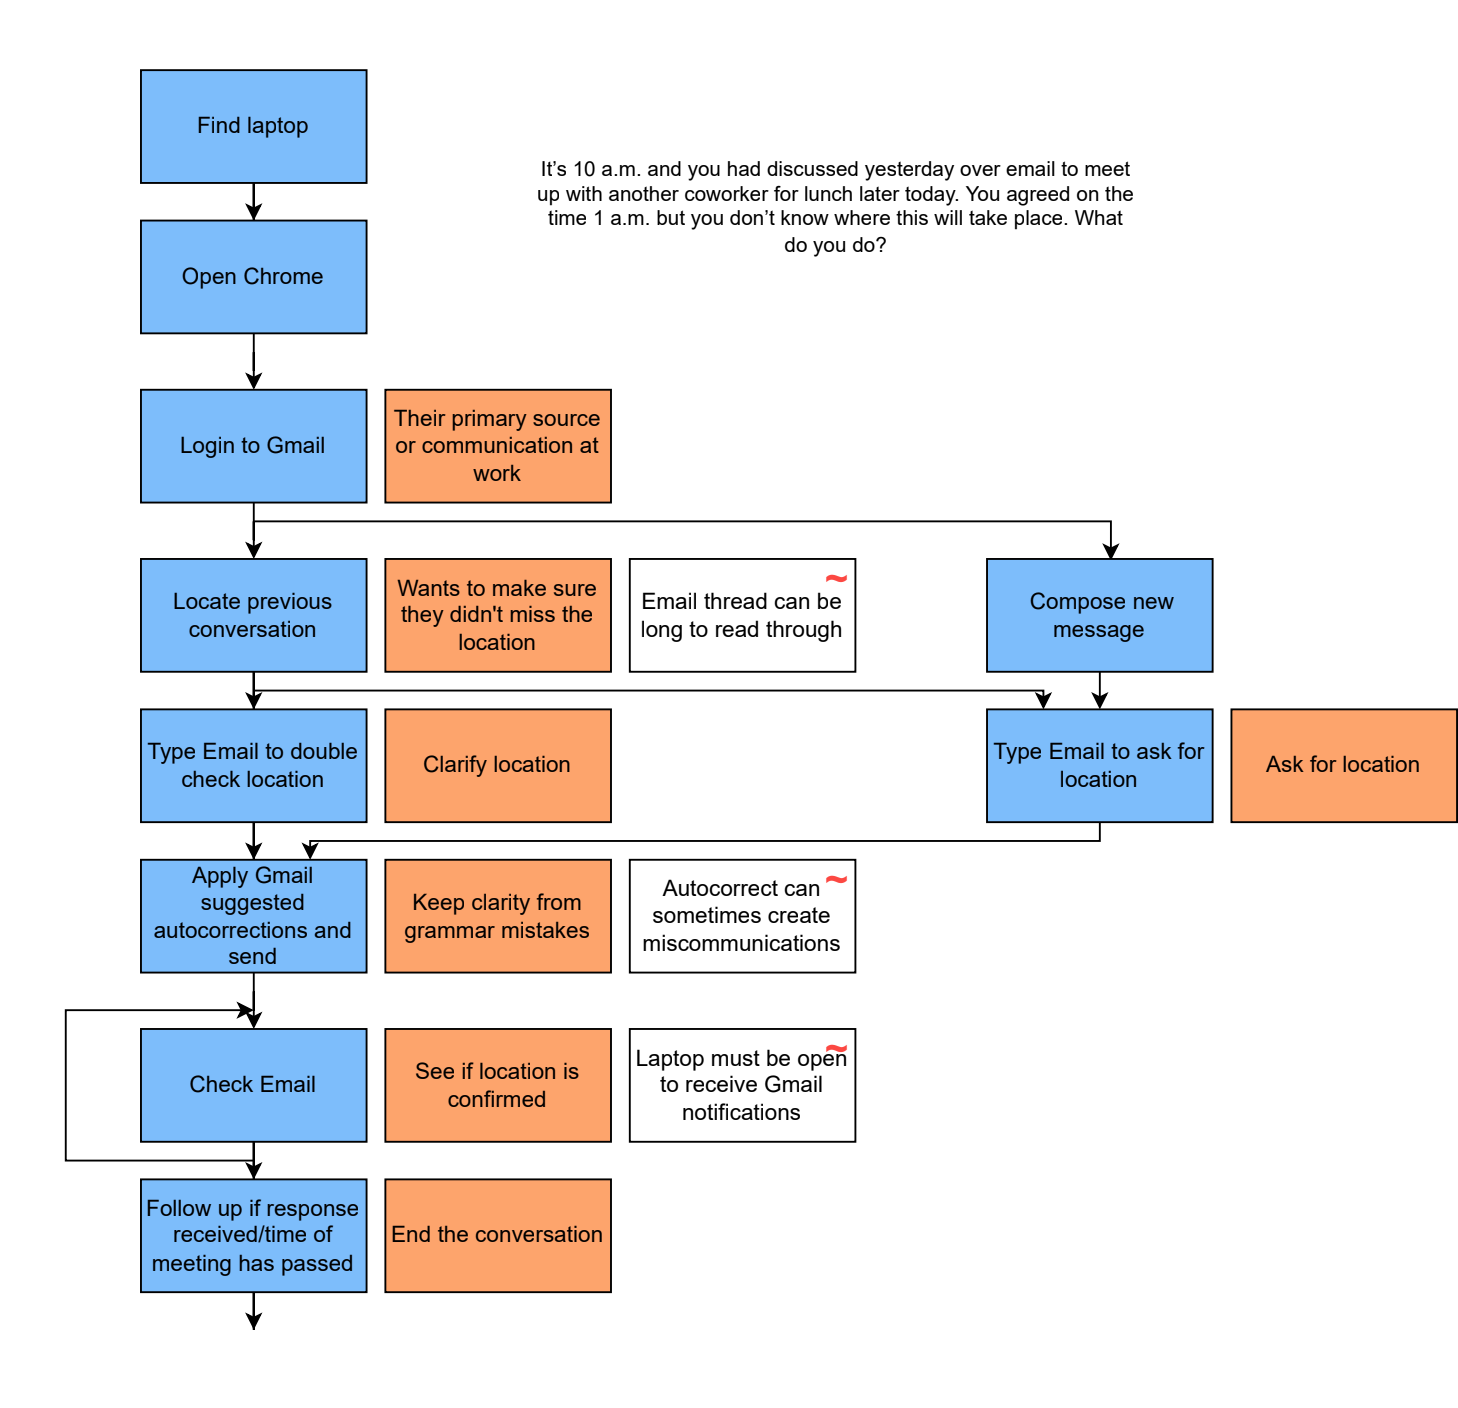
\includegraphics[width=0.5\linewidth]{ {./figures/IndividualSequenceDiagrams/DC-1a.png} }

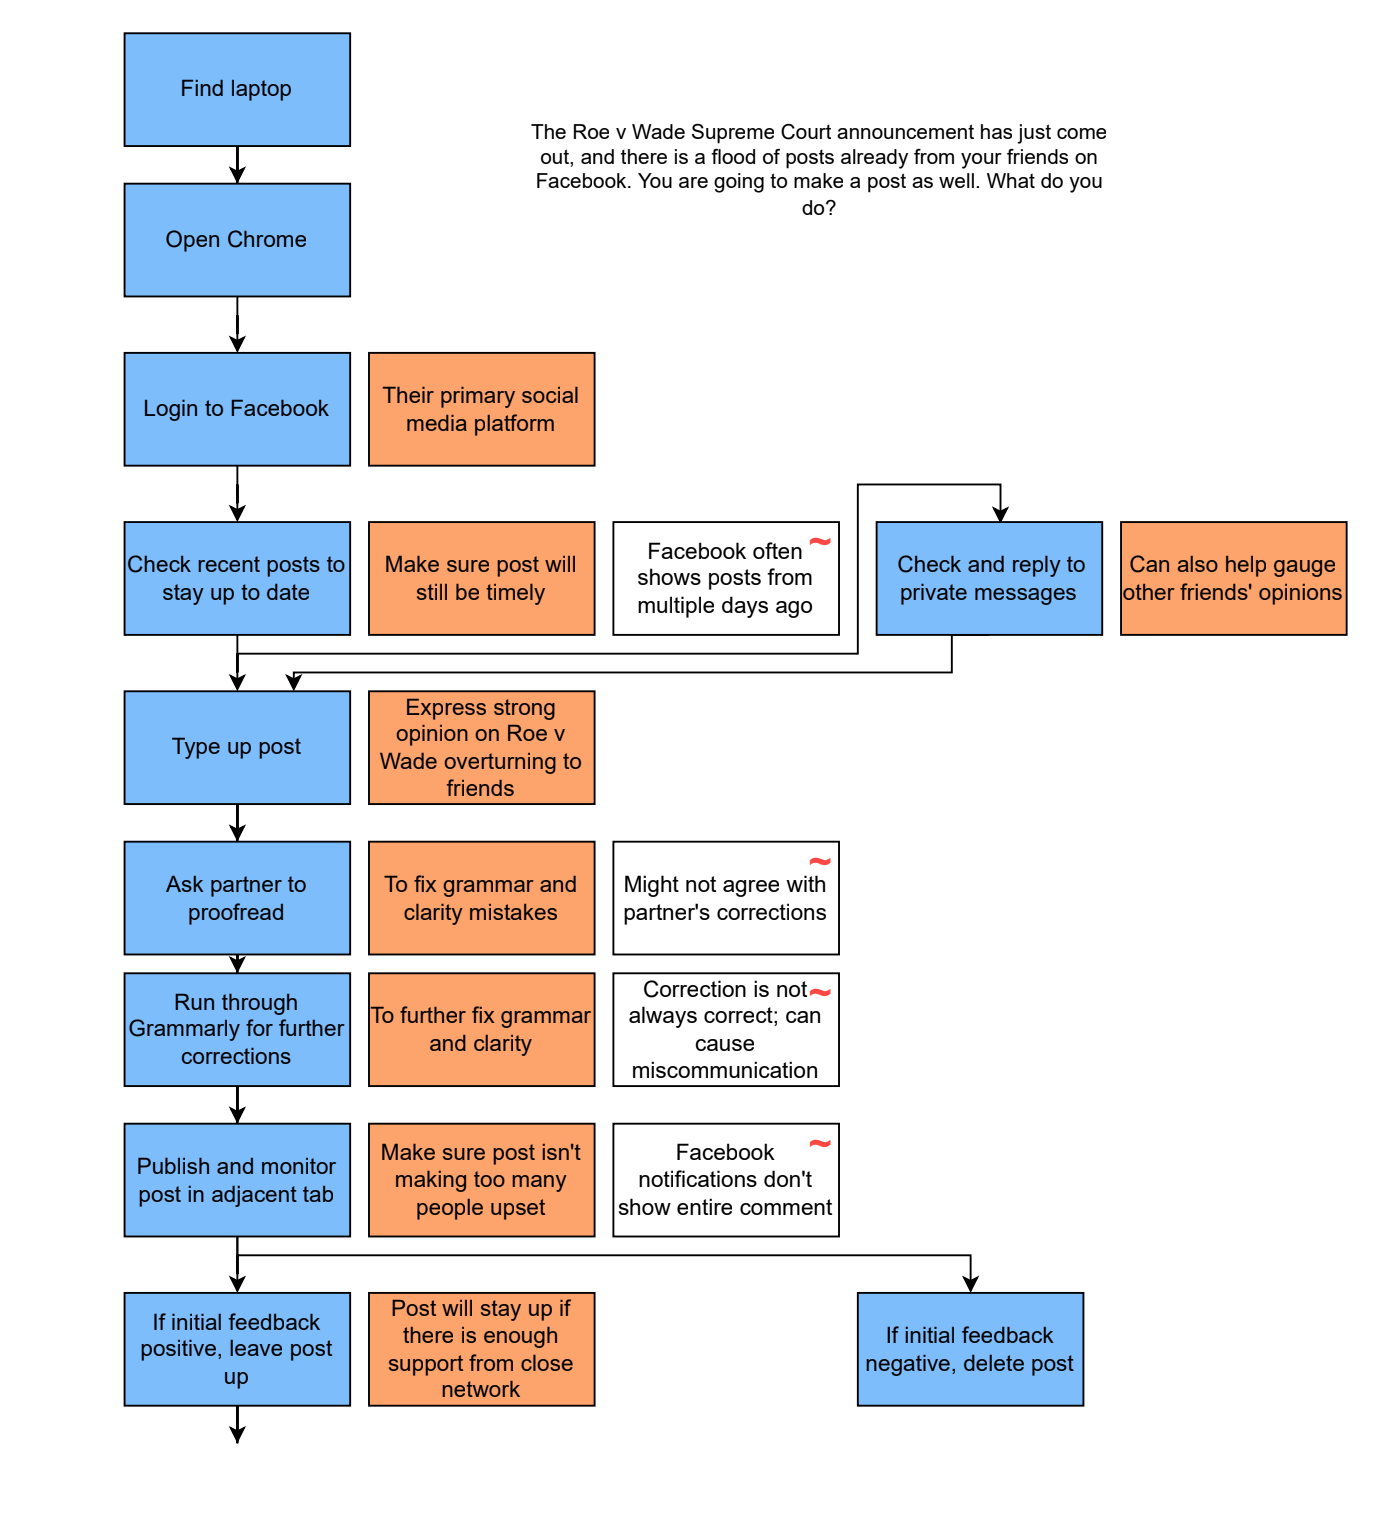
\includegraphics[width=0.5\linewidth]{ {./figures/IndividualSequenceDiagrams/DC-1b.png} }
\end{center}

\subsubsection{ZY}
\begin{center}
\includegraphics[width=0.7\linewidth]{ {./figures/IndividualSequenceDiagrams/ZY-1.png} }

\includegraphics[width=0.7\linewidth]{ {./figures/IndividualSequenceDiagrams/ZY-2.png} }

\includegraphics[width=0.7\linewidth]{ {./figures/IndividualSequenceDiagrams/ZY-3.png} }

\includegraphics[width=0.7\linewidth]{ {./figures/IndividualSequenceDiagrams/ZY-4.png} }
\end{center}

\subsubsection{RC}
\begin{center}
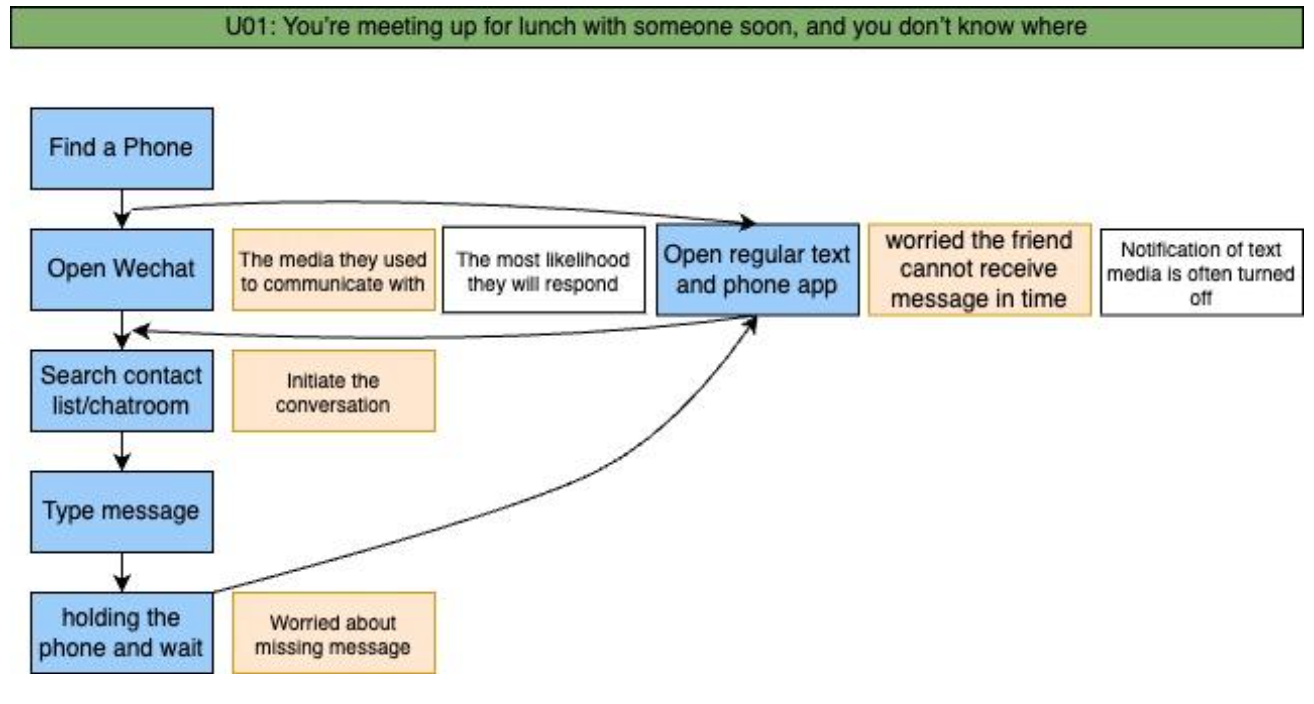
\includegraphics[width=0.7\linewidth]{ {./figures/IndividualSequenceDiagrams/RC-1a.png} }

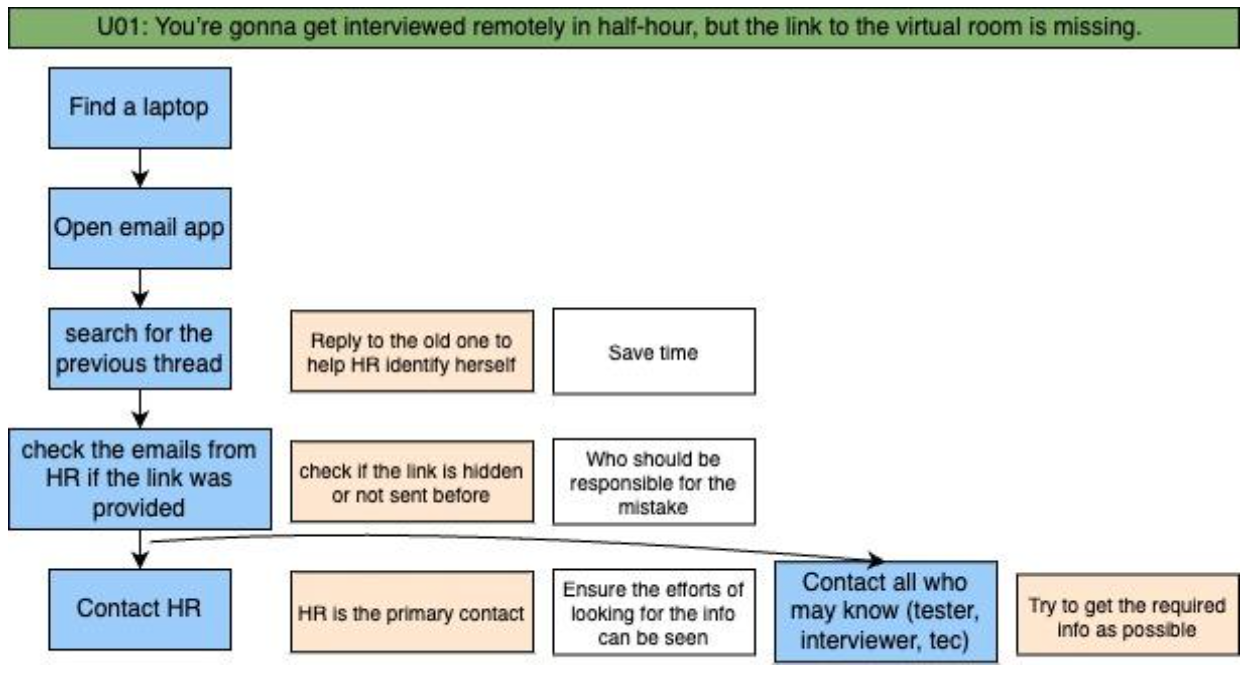
\includegraphics[width=0.7\linewidth]{ {./figures/IndividualSequenceDiagrams/RC-1b.png} }

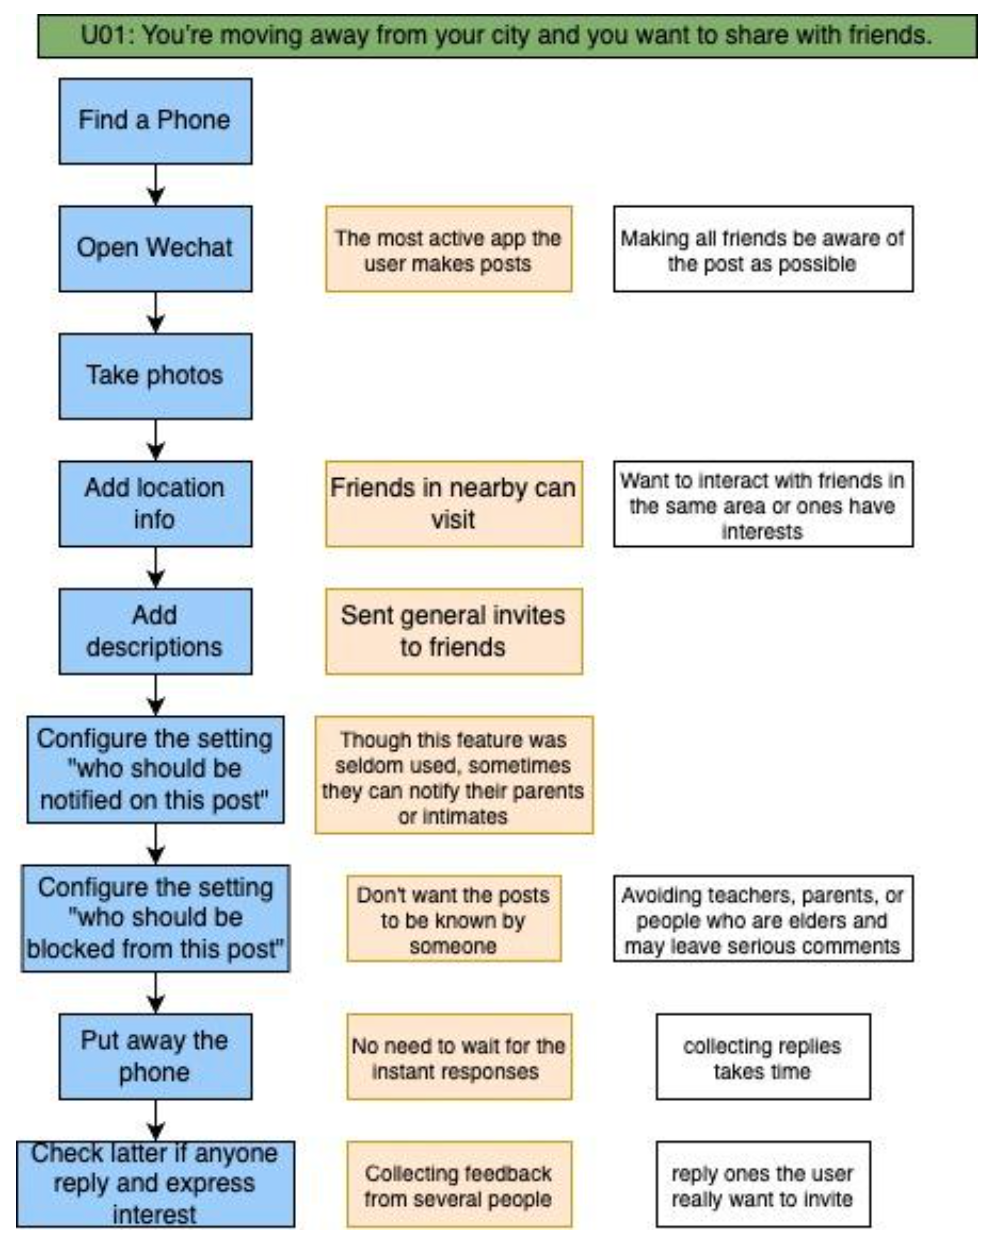
\includegraphics[width=0.7\linewidth]{ {./figures/IndividualSequenceDiagrams/RC-1c.png} }

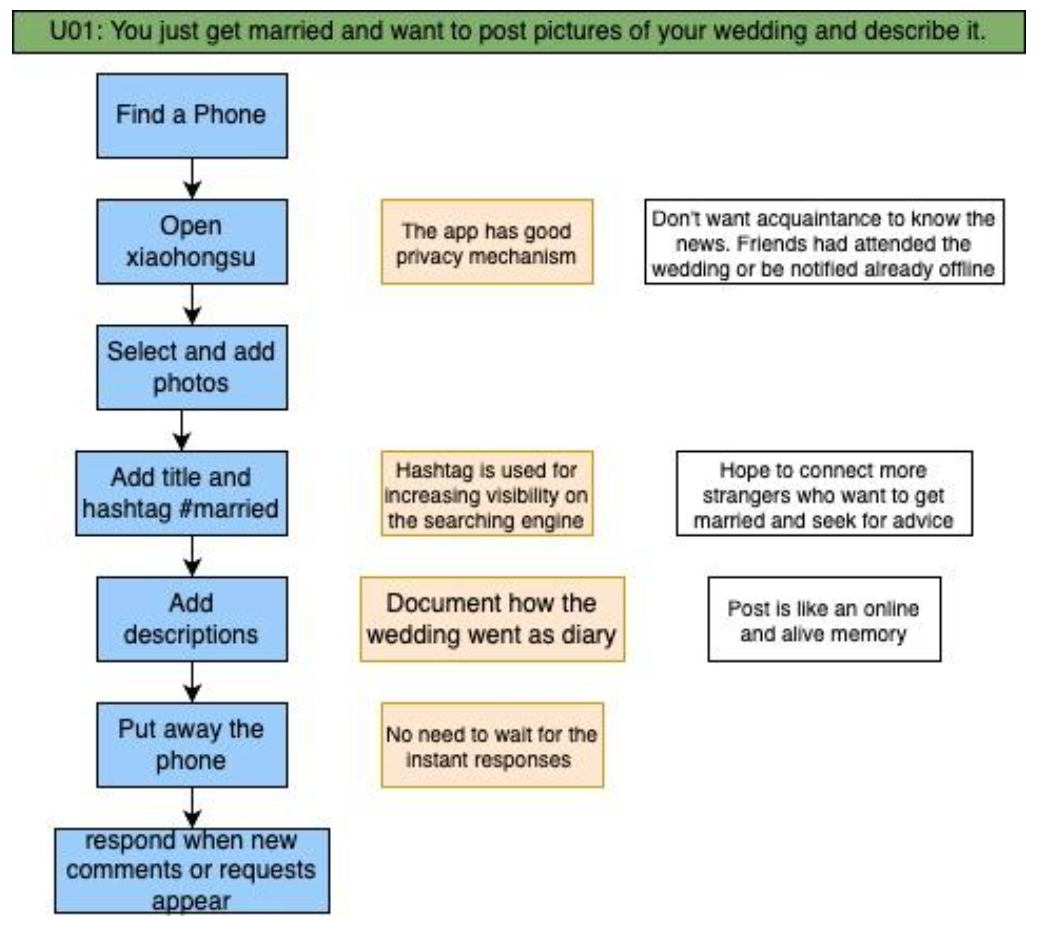
\includegraphics[width=0.7\linewidth]{ {./figures/IndividualSequenceDiagrams/RC-1d.png} }
\end{center}

\subsubsection{BG}
\begin{center}
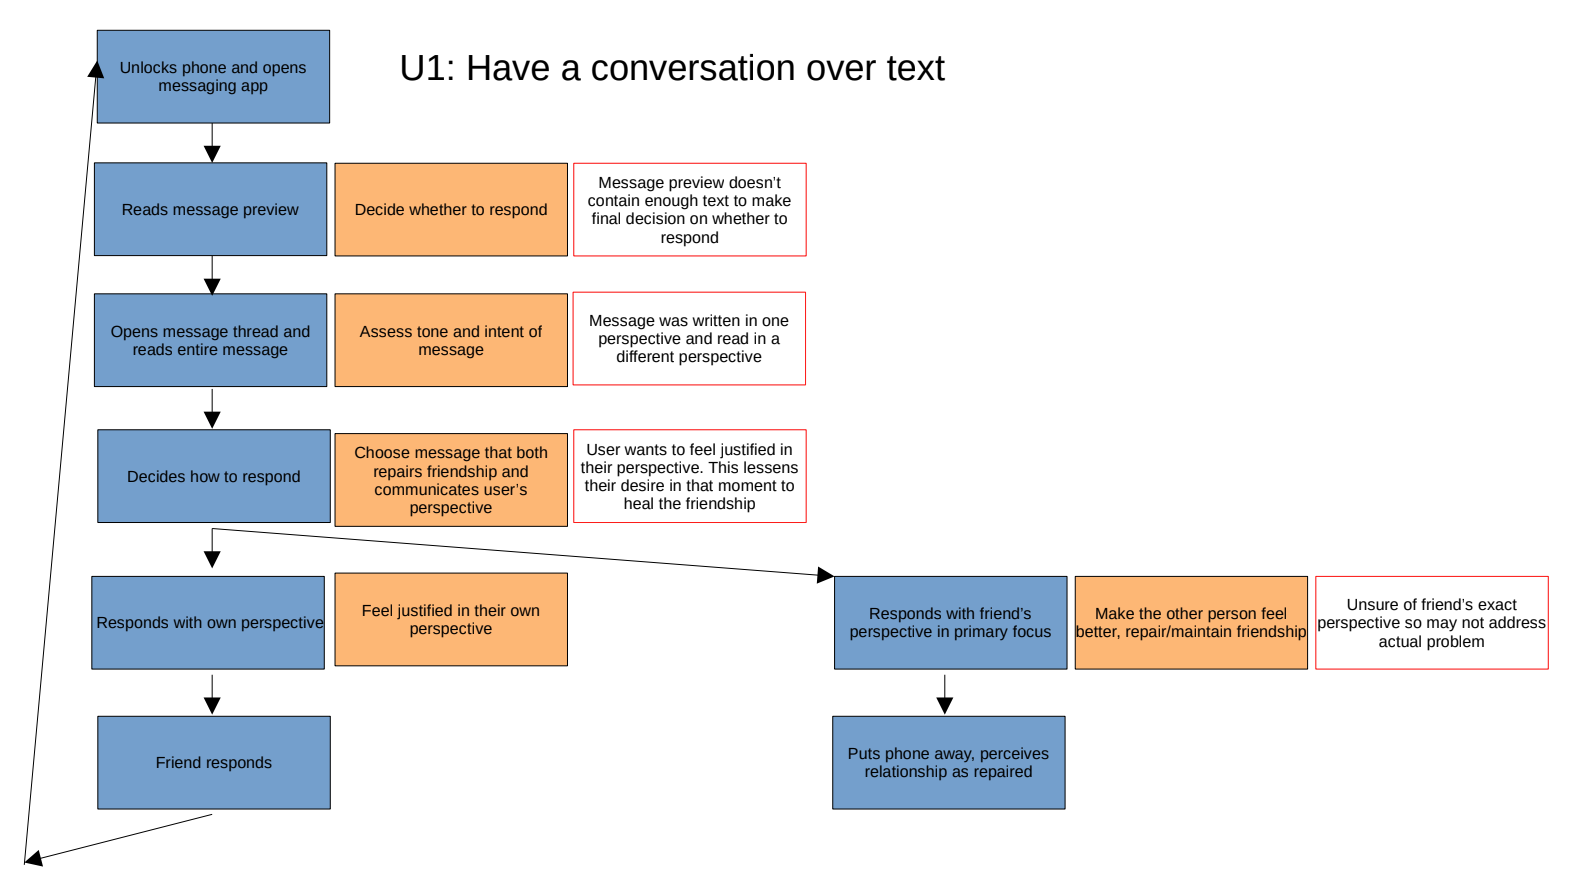
\includegraphics[width=1\linewidth]{ {./figures/IndividualSequenceDiagrams/BG-1a.png} }

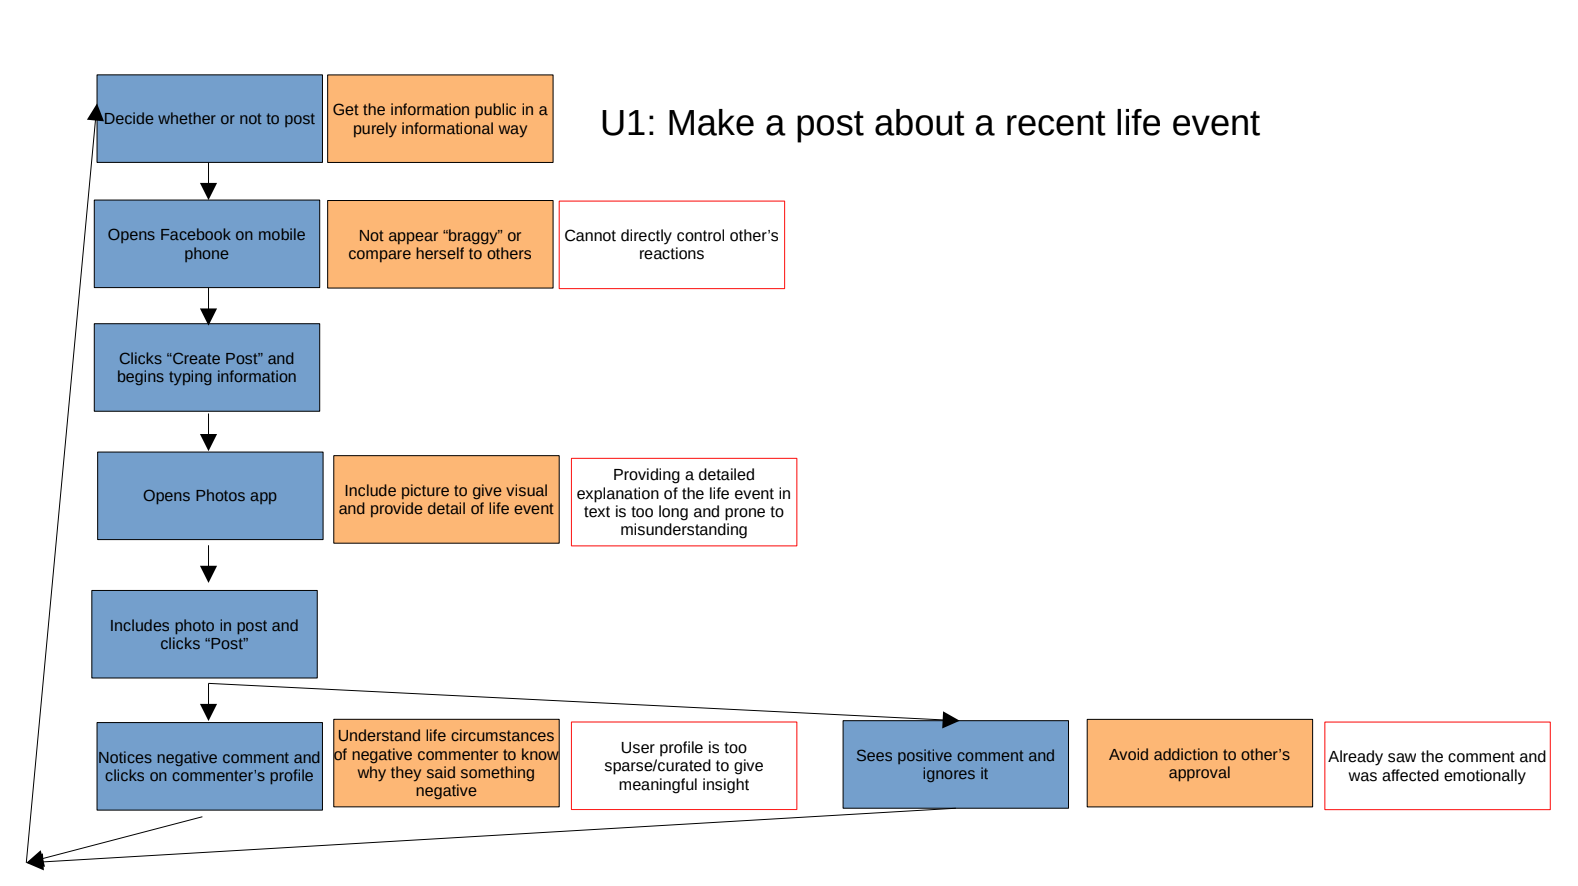
\includegraphics[width=1\linewidth]{ {./figures/IndividualSequenceDiagrams/BG-1b.png} }
\end{center}

\subsubsection{GC}
\begin{center}
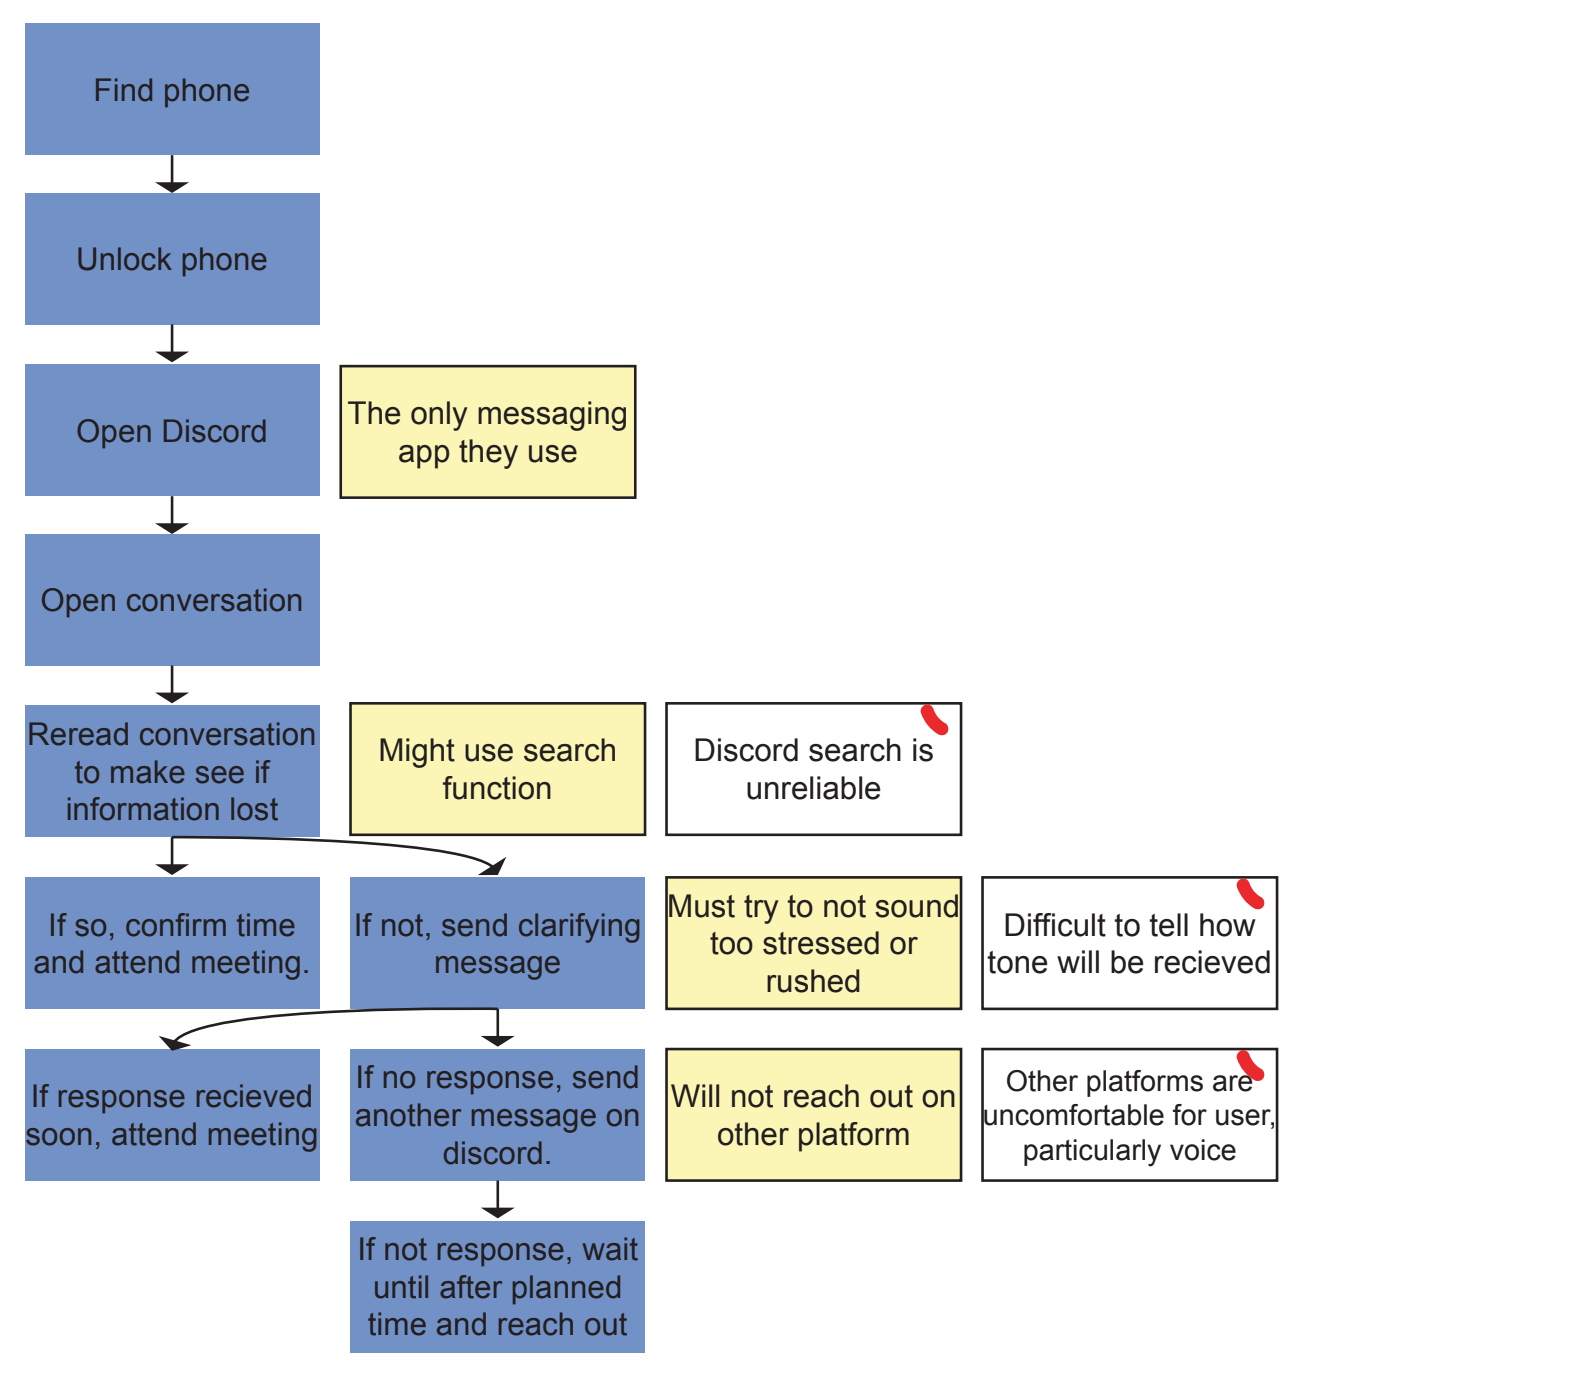
\includegraphics[width=0.8\linewidth]{ {./figures/IndividualSequenceDiagrams/GC-1a.png} }
\end{center}


\subsection{Individual Flow Diagrams}
\label{IFlowDiag}

\subsubsection{DC}
\begin{center}
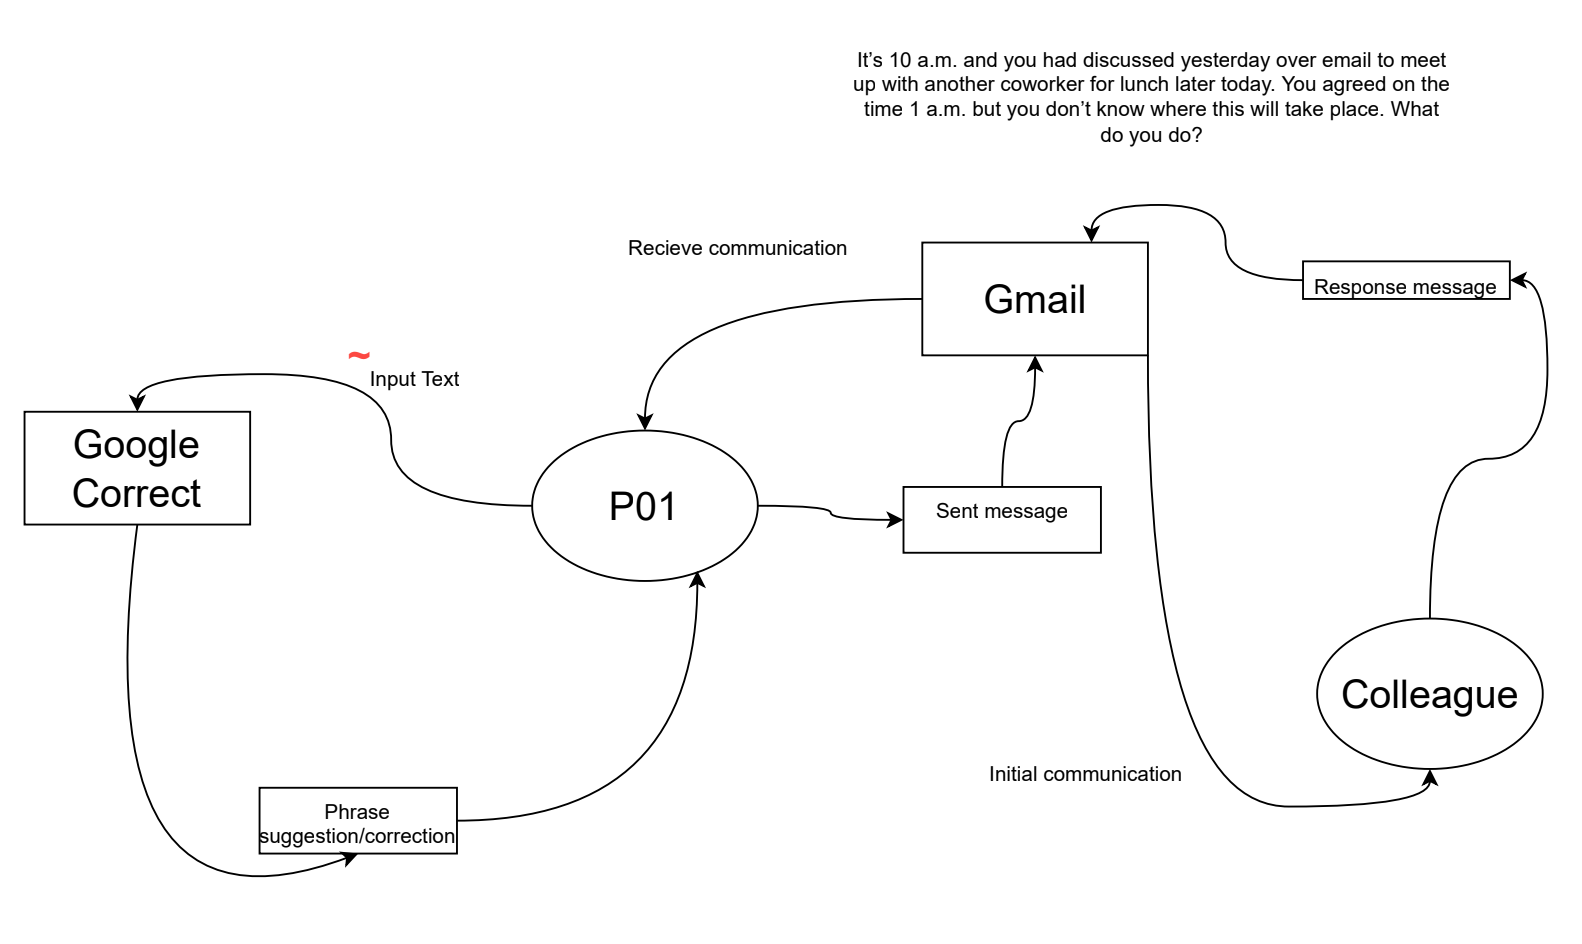
\includegraphics[width=0.7\linewidth]{ {./figures/IndividualFlowDiagrams/DC-2a.png} }

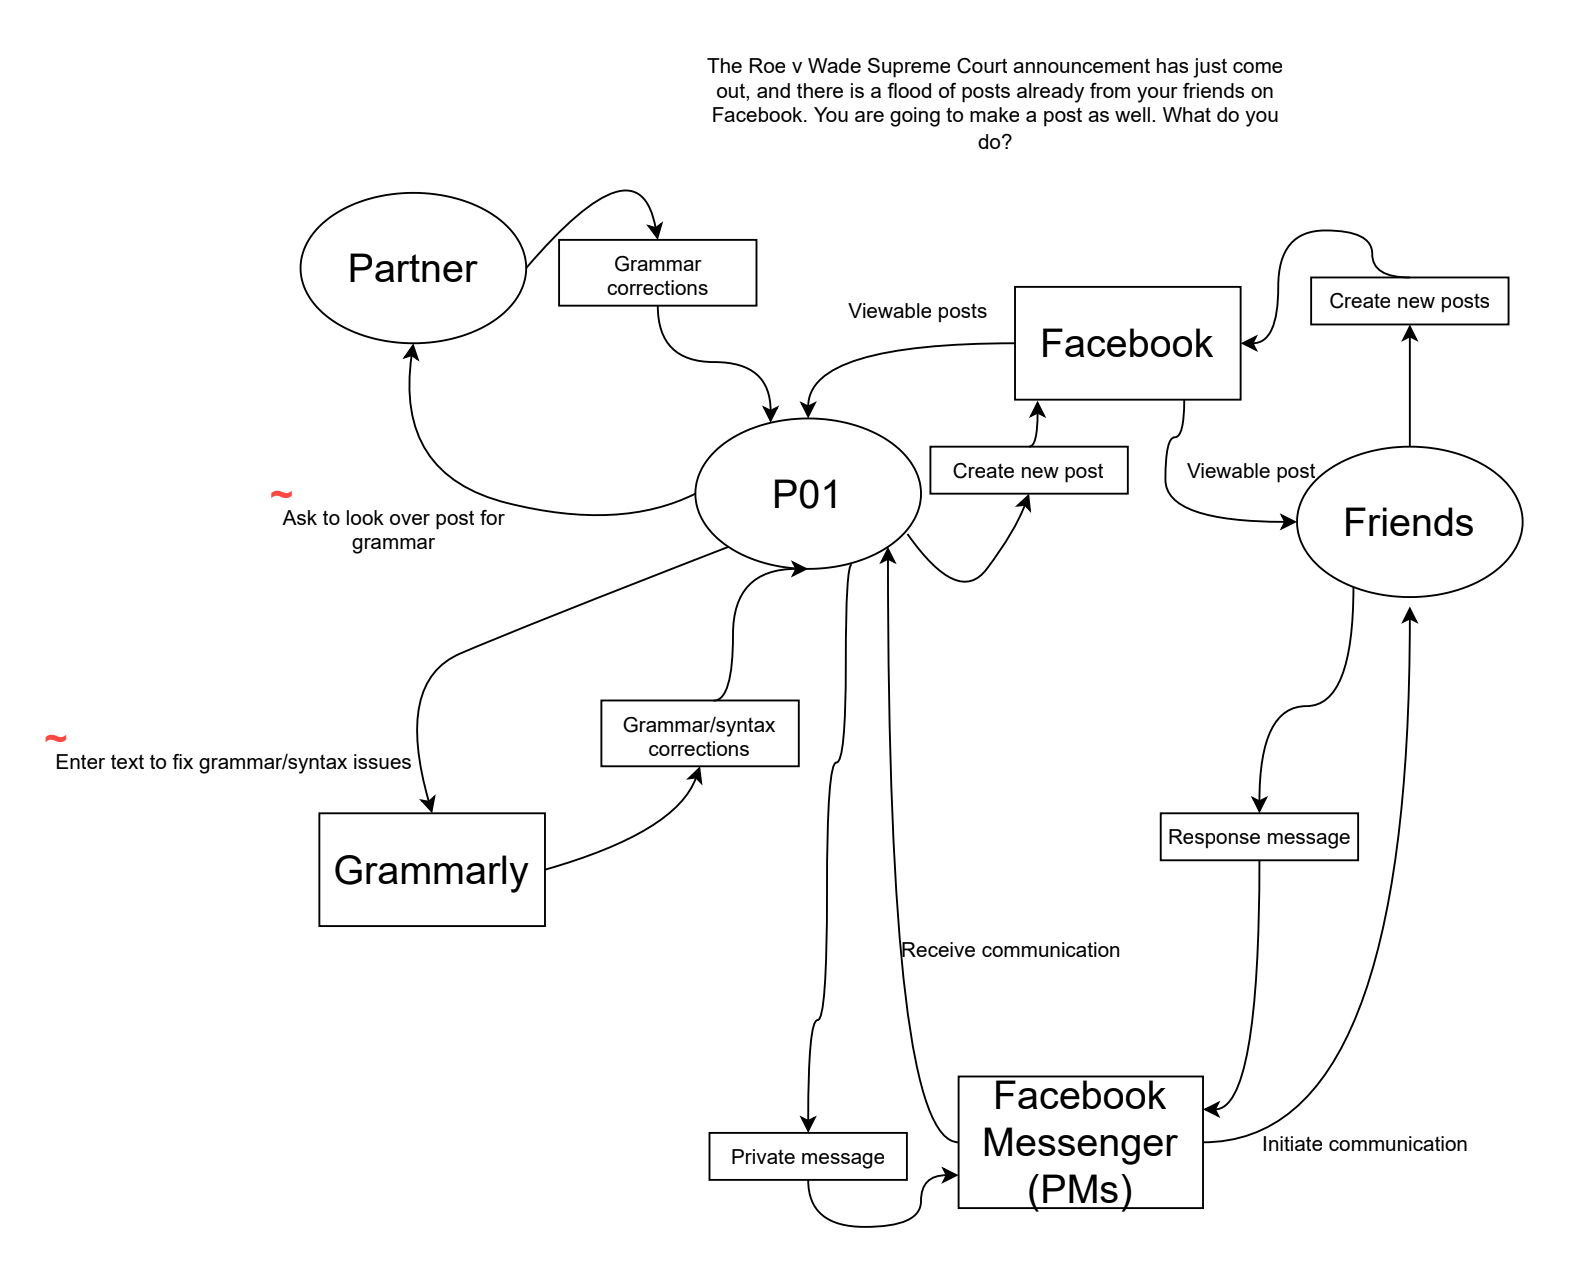
\includegraphics[width=0.7\linewidth]{ {./figures/IndividualFlowDiagrams/DC-2b.png} }
\end{center}


\subsubsection{ZY}
\begin{center}
\includegraphics[width=0.7\linewidth]{ {./figures/IndividualFlowDiagrams/ZY-1.png} }

\includegraphics[width=0.7\linewidth]{ {./figures/IndividualFlowDiagrams/ZY-2.png} }

\includegraphics[width=0.7\linewidth]{ {./figures/IndividualFlowDiagrams/ZY-3.png} }

\includegraphics[width=0.7\linewidth]{ {./figures/IndividualFlowDiagrams/ZY-4.png} }
\end{center}

\subsubsection{RC}
\begin{center}
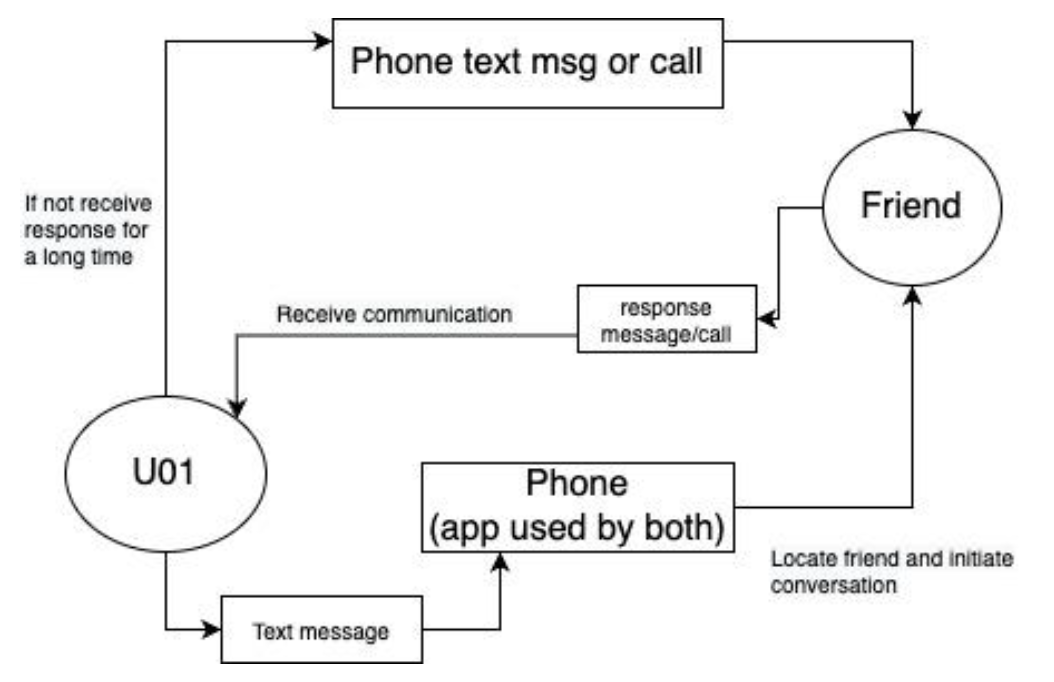
\includegraphics[width=0.7\linewidth]{ {./figures/IndividualFlowDiagrams/RC-2a.png} }

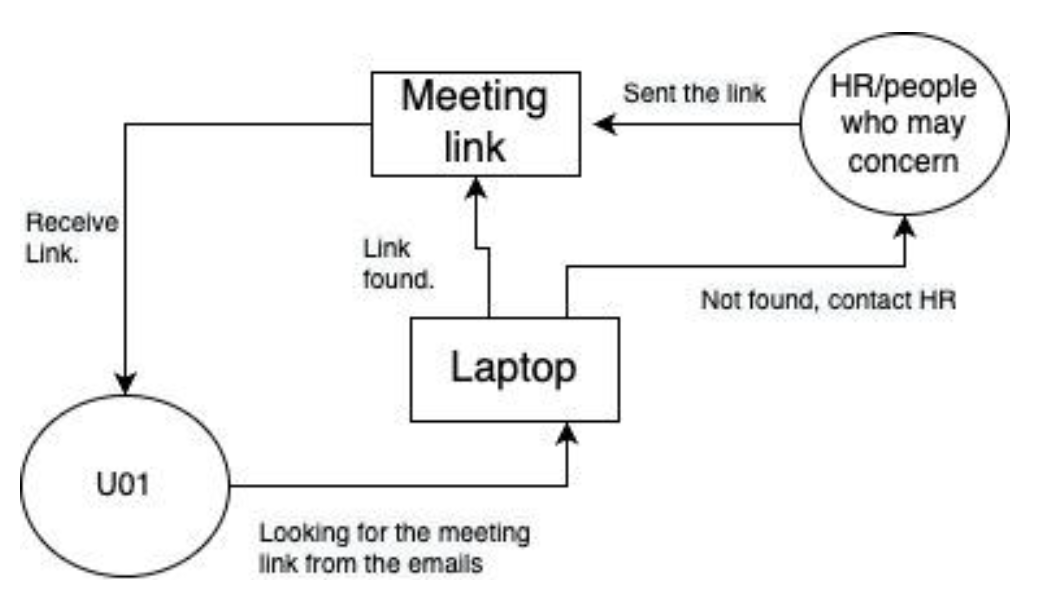
\includegraphics[width=0.7\linewidth]{ {./figures/IndividualFlowDiagrams/RC-2b.png} }

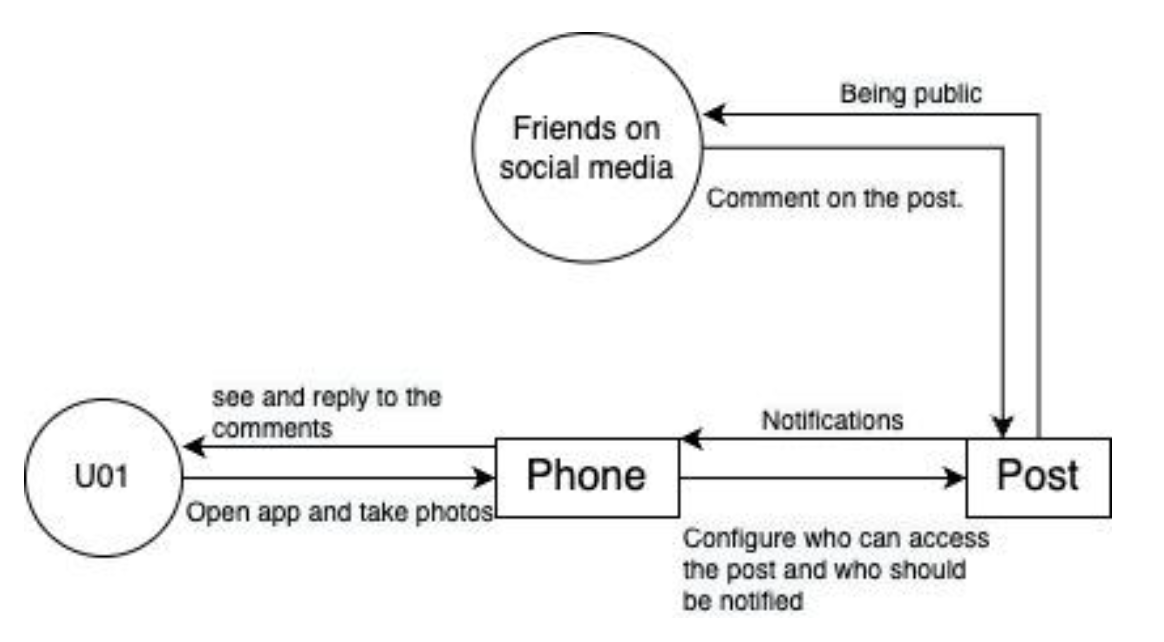
\includegraphics[width=0.7\linewidth]{ {./figures/IndividualFlowDiagrams/RC-2c.png} }

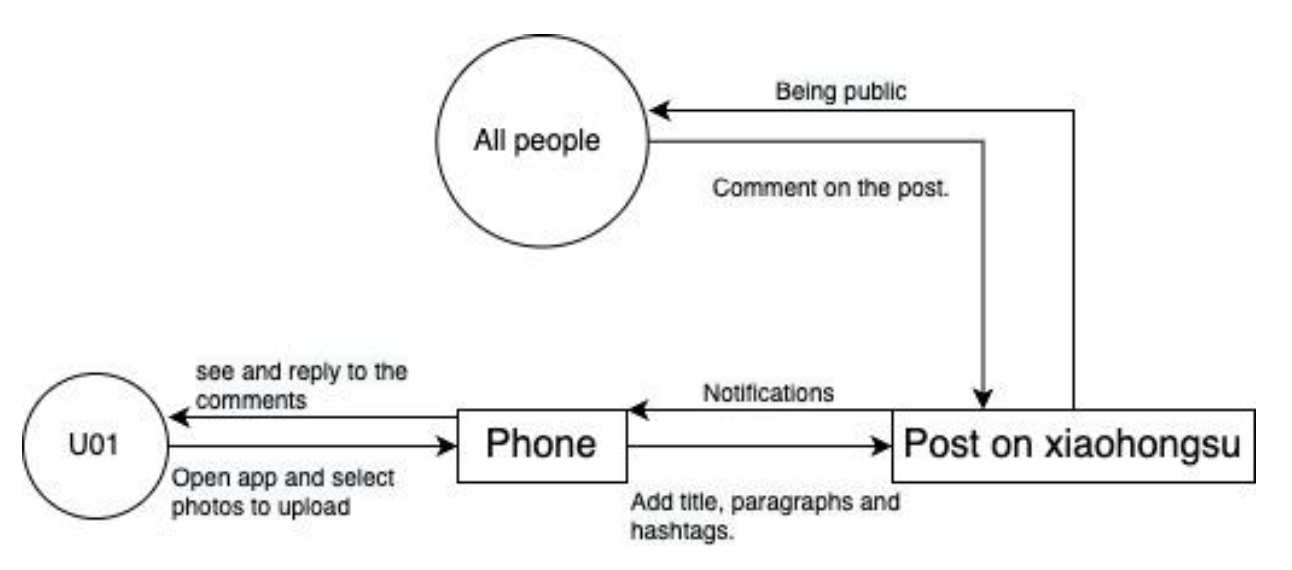
\includegraphics[width=0.7\linewidth]{ {./figures/IndividualFlowDiagrams/RC-2d.png} }
\end{center}

\subsubsection{BG}
\begin{center}
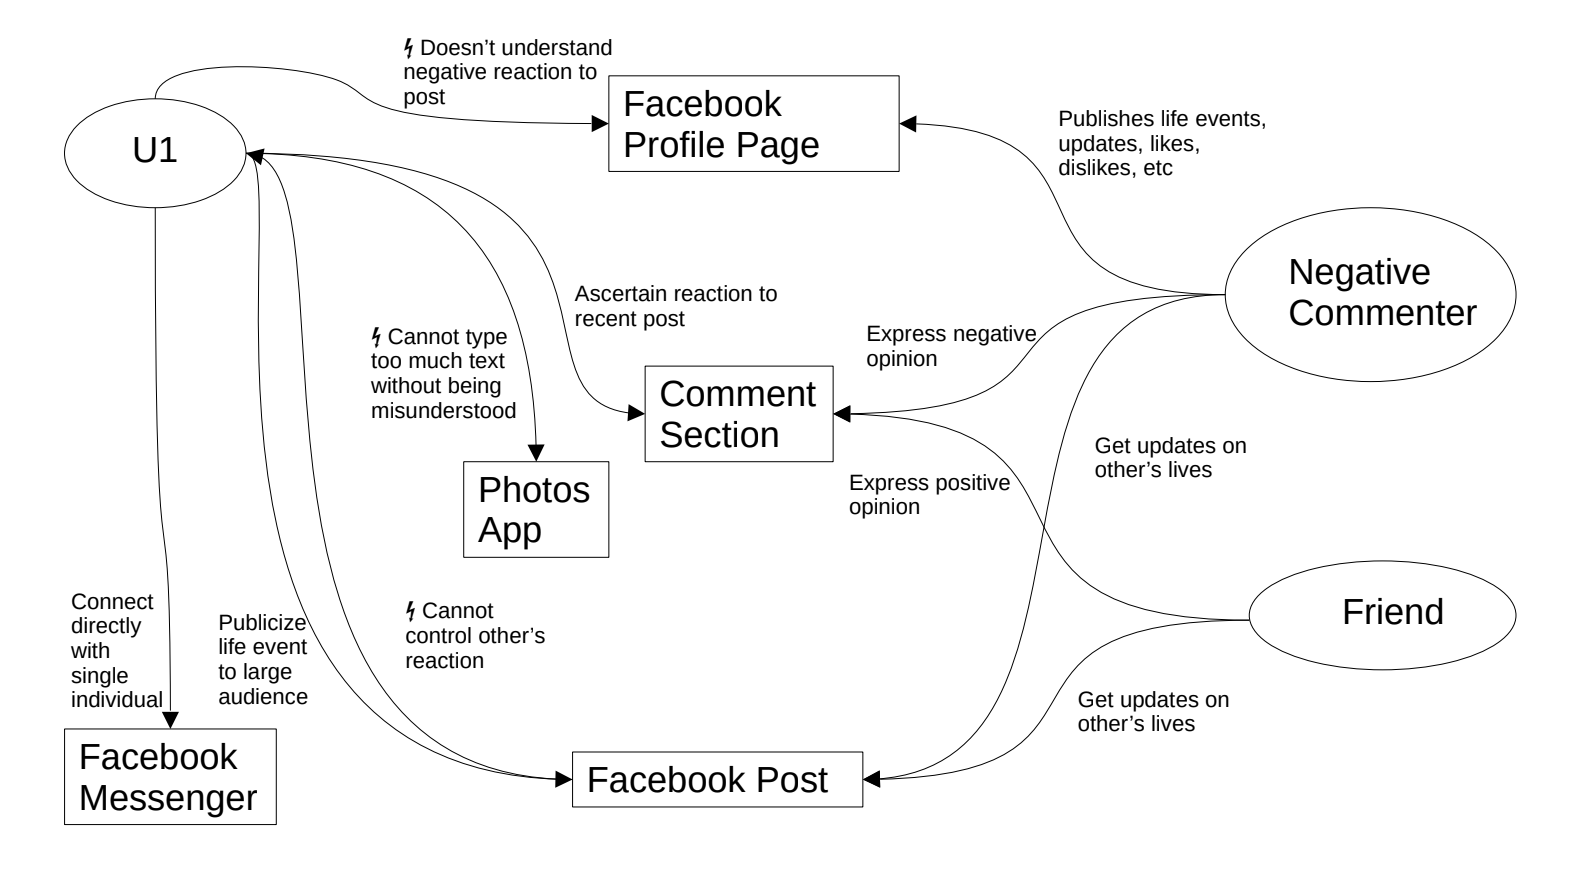
\includegraphics[width=1\linewidth]{ {./figures/IndividualFlowDiagrams/BG-2a.png} }

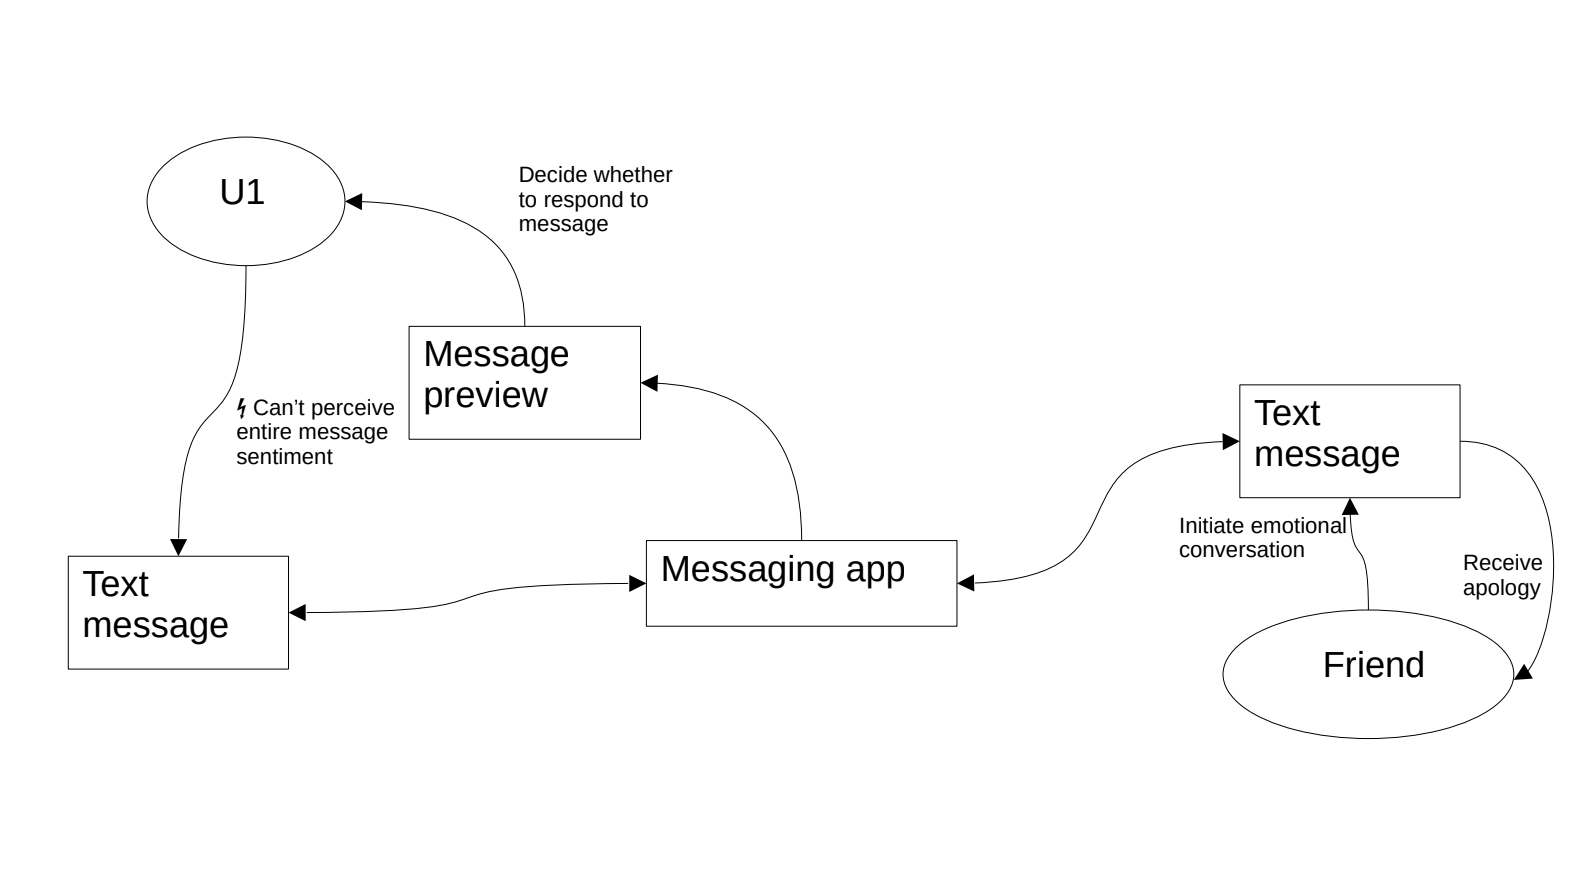
\includegraphics[width=1\linewidth]{ {./figures/IndividualFlowDiagrams/BG-2b.png} }
\end{center}

\subsubsection{GC}
\begin{center}
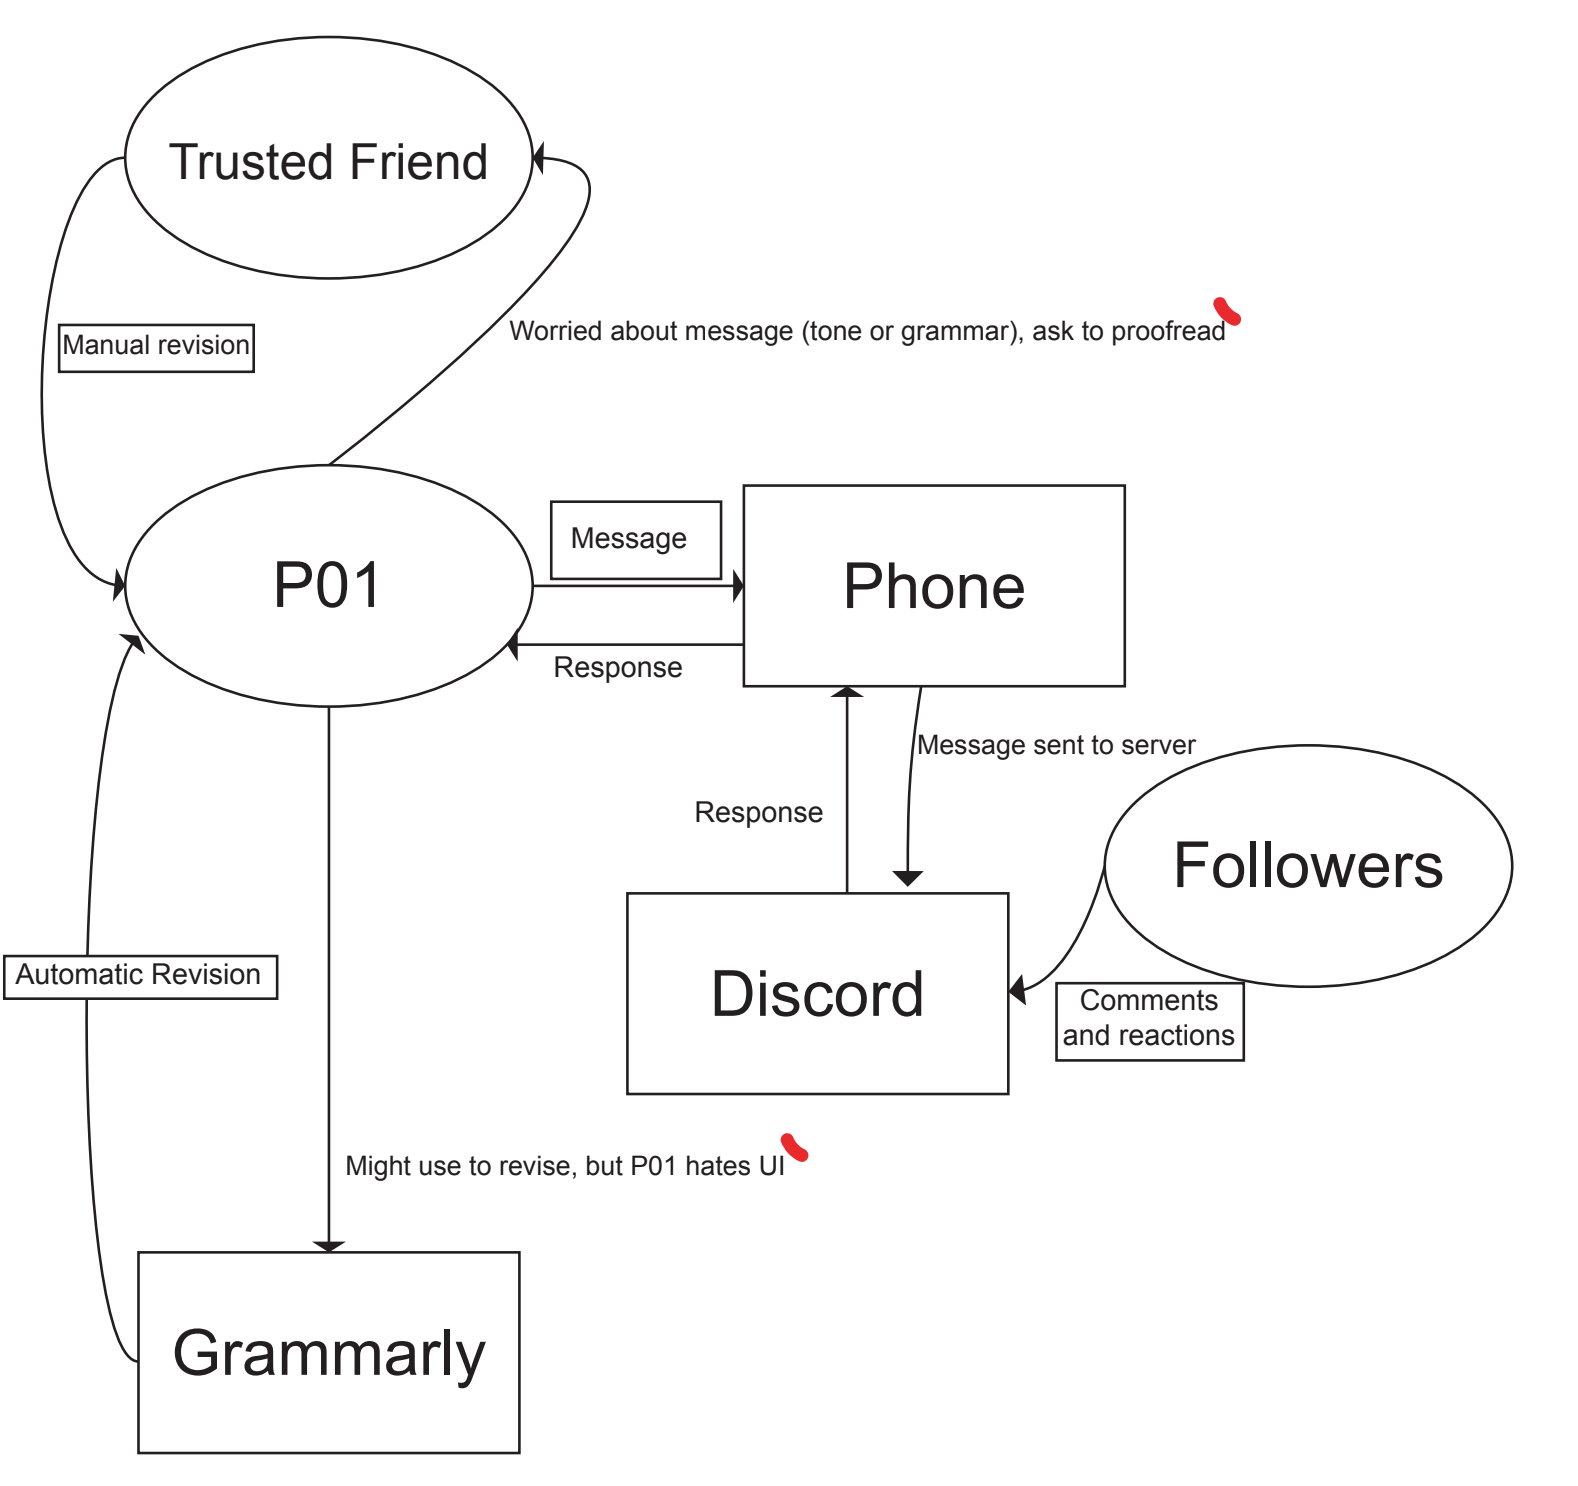
\includegraphics[width=0.8\linewidth]{ {./figures/IndividualFlowDiagrams/GC-2a.png} }
\end{center}


\subsection{Consolidated Sequence Diagrams}

% \begin{figure*}[h]
\begin{center}
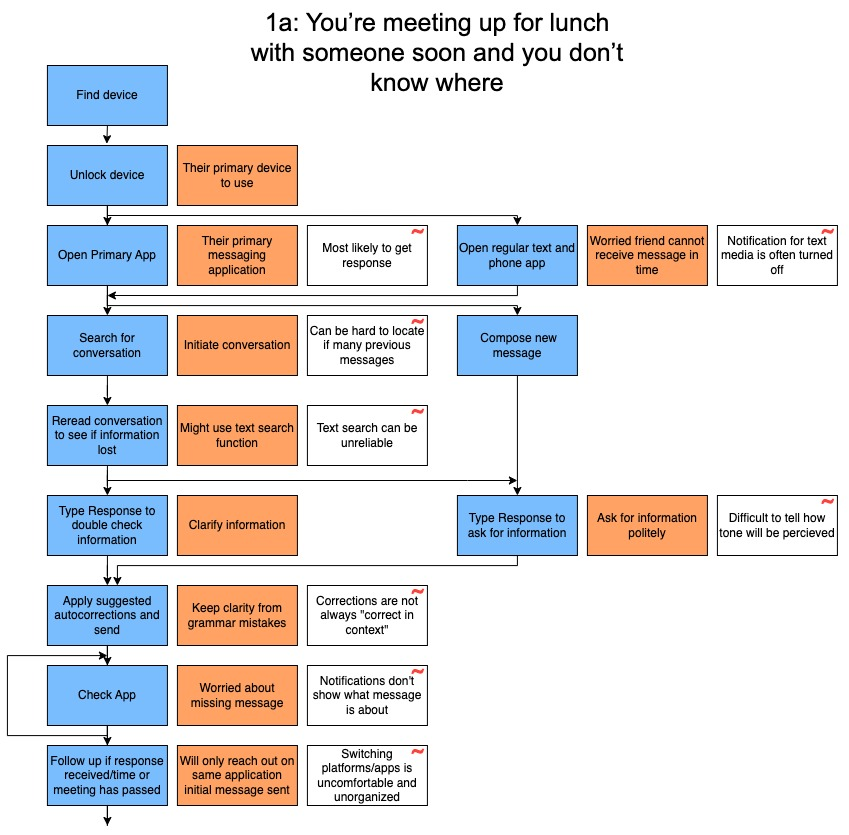
\includegraphics[width=0.9\linewidth]{
% {./figures/ConsolidateSeqDiagrams/1aSequenceDiagram.jpg} }
{./figures/ConsolidateSeqDiagrams/Updated_seq.png} }
% \caption{Bar charts for the questions in Tools section, including the options, number of responses and the percentage of distribution.}
\label{fig:tools}
\Description{}
\end{center}
% \end{figure*}


\subsection{Consolidated Flow Diagrams}

Simplified Flow Diagram

\begin{center}
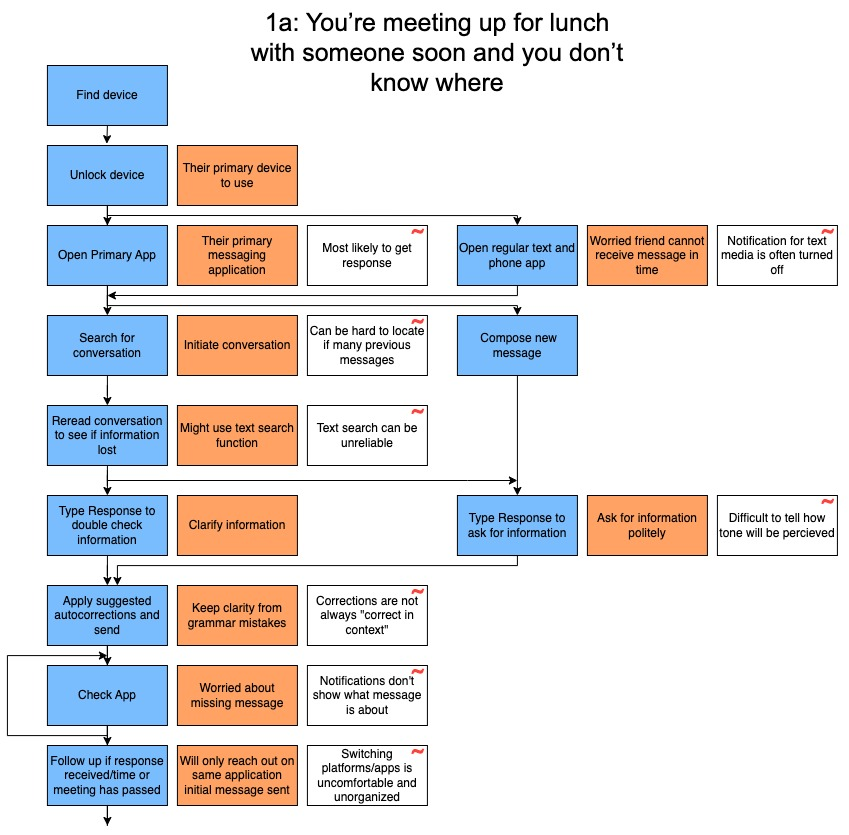
\includegraphics[width=0.9\linewidth]{
% {./figures/ConsolidateSeqDiagrams/1aSequenceDiagram.jpg} }
{./figures/ConsolidateFloDiagrams/flow.png} }
% \caption{Bar charts for the questions in Tools section, including the options, number of responses and the percentage of distribution.}
\label{fig:tools}
\Description{}
\end{center}

Detailed Flow Diagrams

\begin{center}
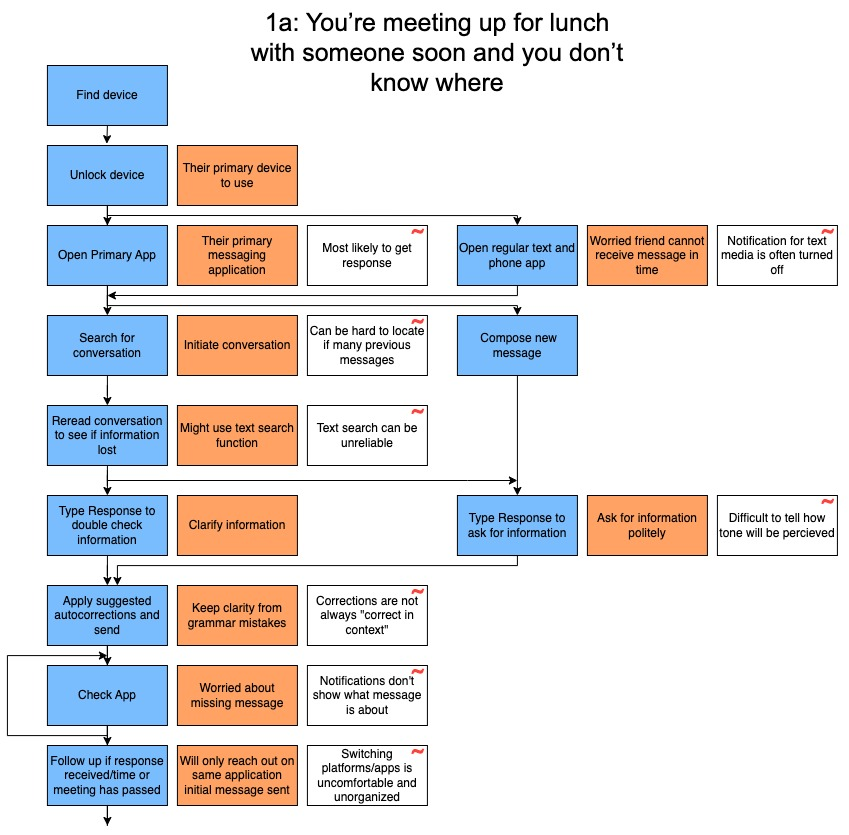
\includegraphics[width=0.9\linewidth]{
% {./figures/ConsolidateSeqDiagrams/1aSequenceDiagram.jpg} }
{./figures/ConsolidateFloDiagrams/Part1FloDiagram.png} }
% \caption{Bar charts for the questions in Tools section, including the options, number of responses and the percentage of distribution.}
\label{fig:tools}
\Description{}
\end{center}

\begin{center}
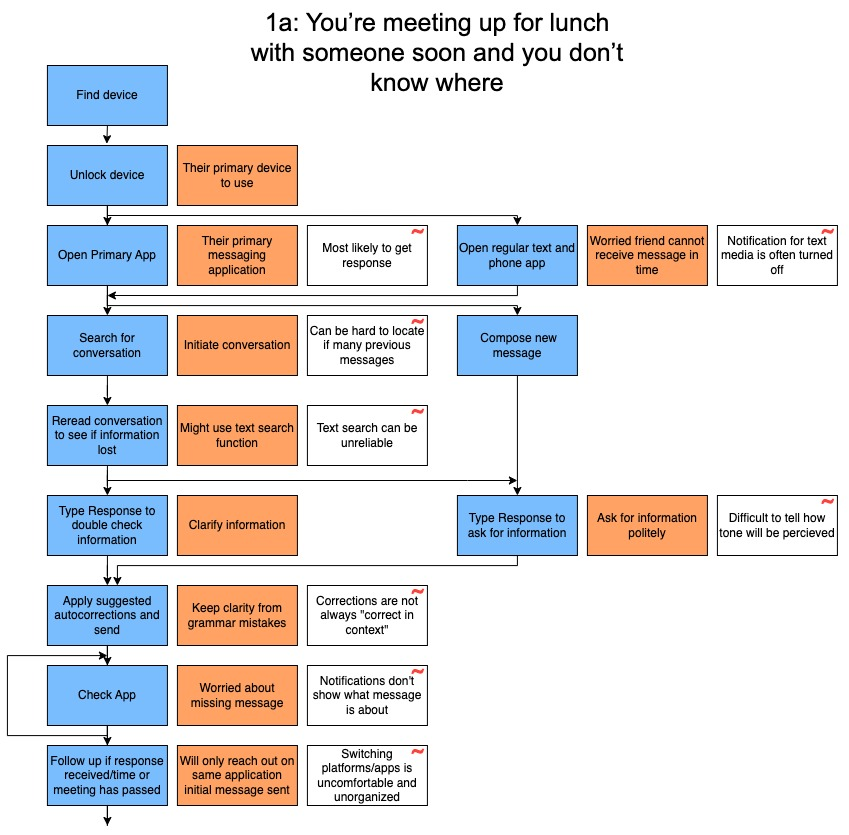
\includegraphics[width=0.9\linewidth]{
% {./figures/ConsolidateSeqDiagrams/1aSequenceDiagram.jpg} }
{./figures/ConsolidateFloDiagrams/Part2FloDiagram.png} }
% \caption{Bar charts for the questions in Tools section, including the options, number of responses and the percentage of distribution.}
\label{fig:tools}
\Description{}
\end{center}


\subsection{Affinity Diagram}

\begin{center}
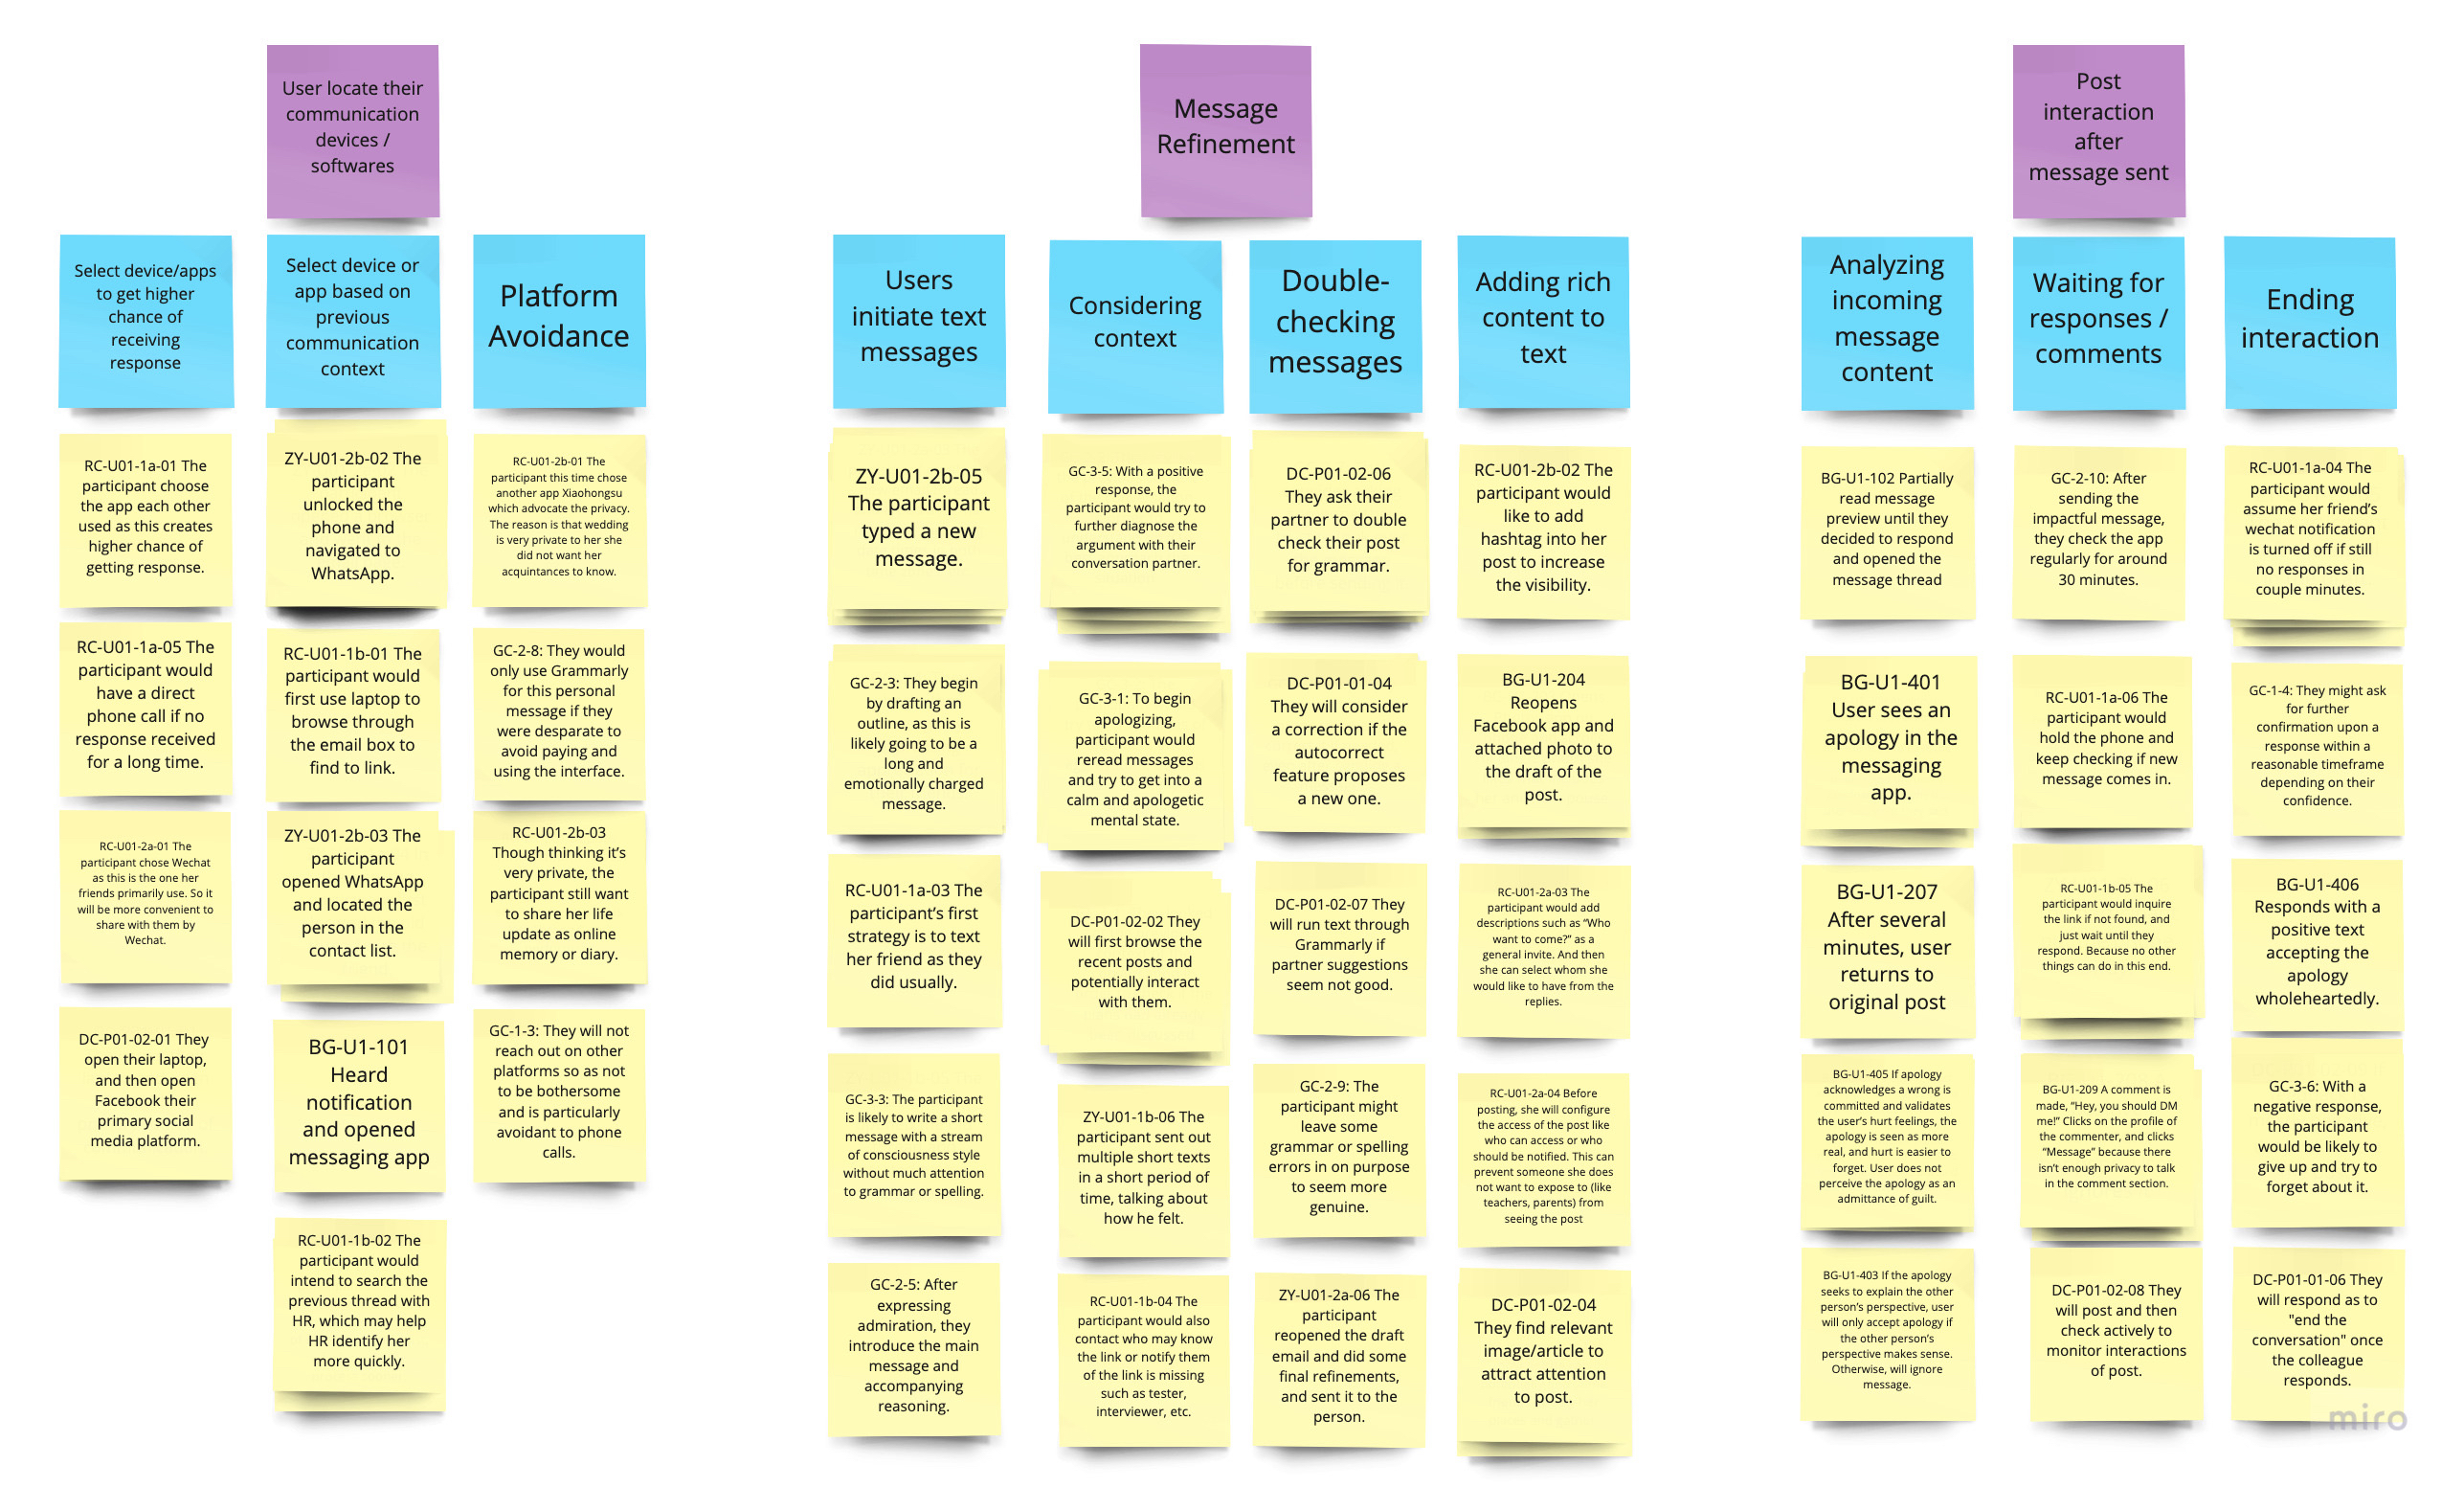
\includegraphics[width=1\linewidth]{
{./figures/Affinity.jpeg} }
% \caption{Bar charts for the questions in Tools section, including the options, number of responses and the percentage of distribution.}
\label{fig:tools}
\Description{}
\end{center}

\section{Low Fidelity Prototypes}

\subsection{Individual Personas}
\label{appendix:personas}
\subsubsection{DC}

The persona is a hypothetical (not-real) 17-year-old foreign exchange student named Sasha who is at an American high school and trying to befriend new people. He has spoken Ukrainian all his life, but he only started learning English in the 4th grade. Some new friends have invited him to a “movie night”, but Sasha is a little bit behind in school and wants to send them a text to delay/let his friends know he isn’t coming. He wants to do this in such a way that he doesn’t come off
“lonely” or “sad”, but instead “friendly” or “understanding”.

Our context of use is looking to find a way to help people for “text corrections in more informal situations”, where also many seem to prefer to check their texts/emails for other things besides just grammar. Thus, it seems the persona of Sasha appears to
be a person who would benefit from a solution to this problem.

\subsubsection{ZY}
\begin{center}
    %\fbox{
    \includegraphics[
        page=2, 
        clip, 
        trim=2.5cm 15cm 2.5cm 3.5cm,
        width=0.9\textwidth
    ]{figures/Assignment_3/ZY (Individual).pdf}
    %}
    %\caption{Title}
    \label{fig:persona_zy}
\end{center}
\subsubsection{RC}
\label{indiv_persona_rc}

\begin{figure}
\begin{center}
    %\fbox{
    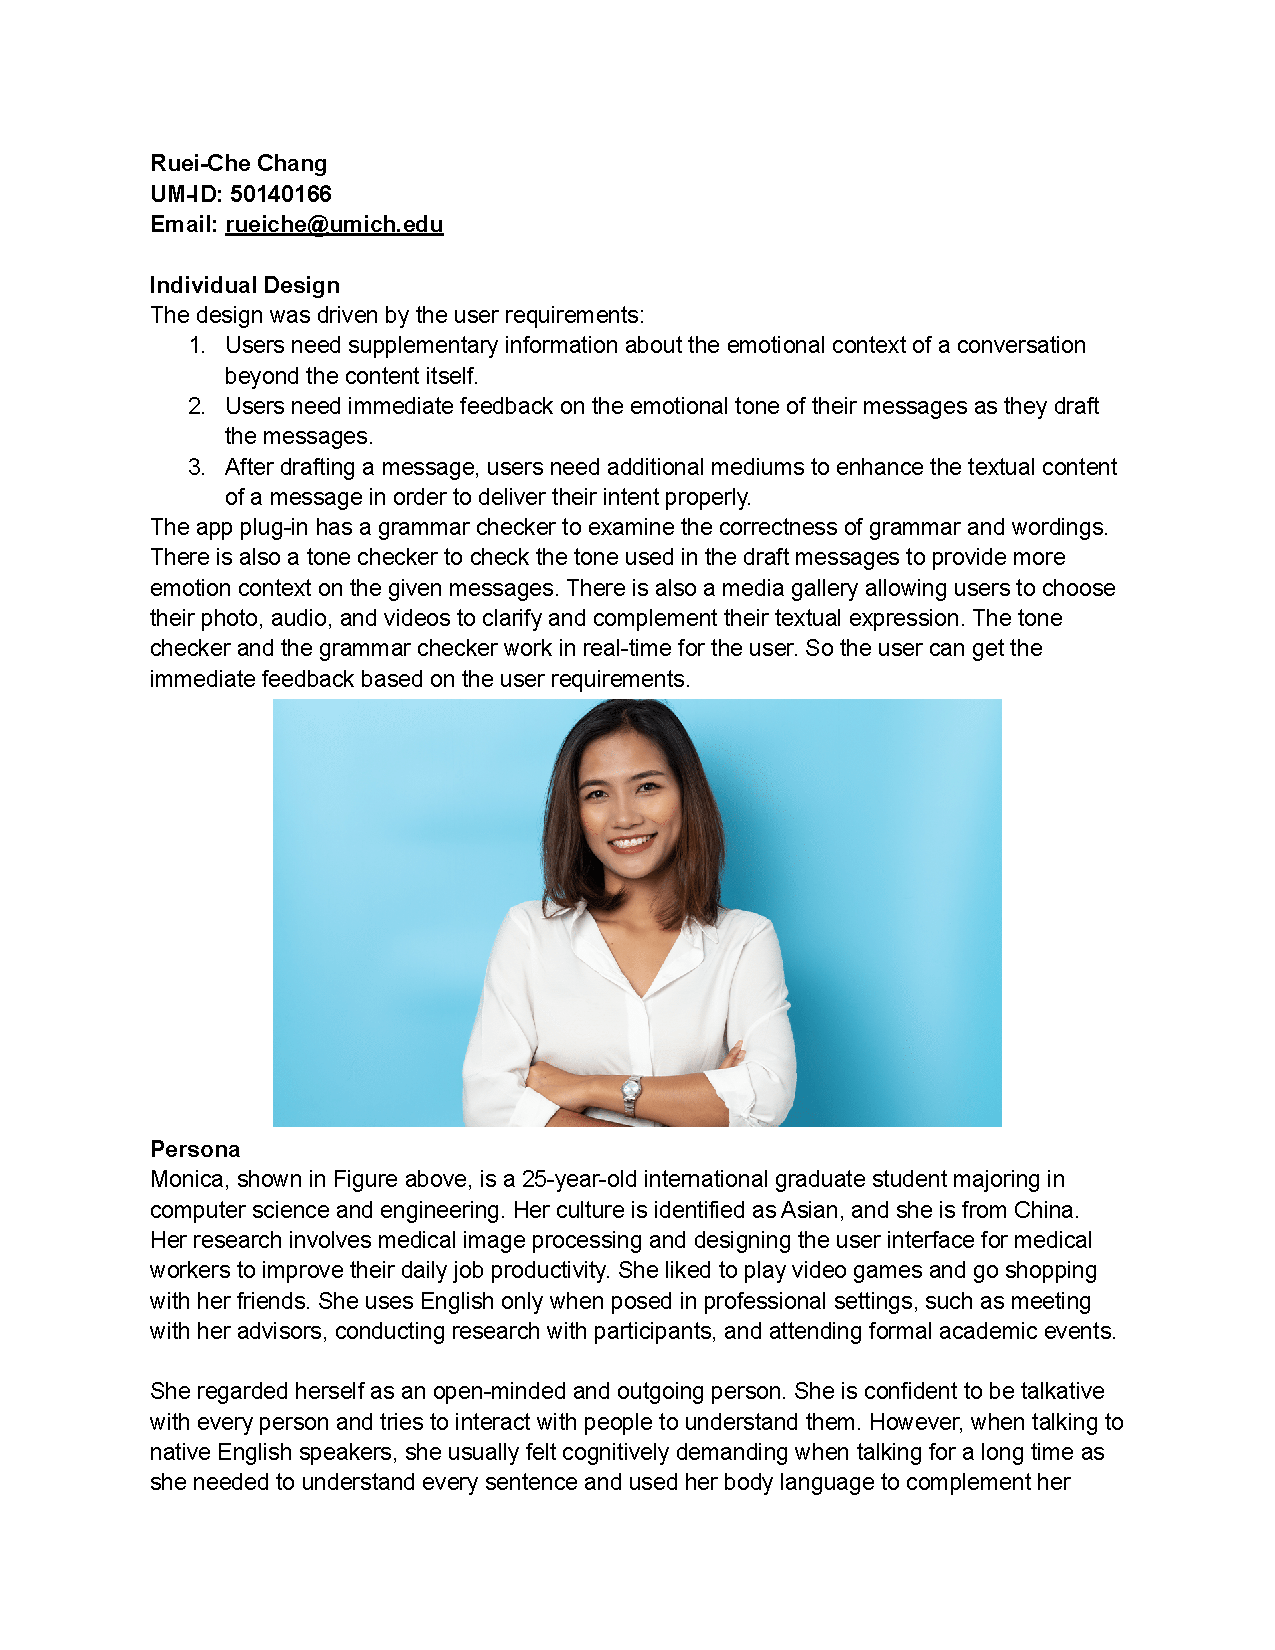
\includegraphics[
        page=1, 
        clip, 
        trim=5.5cm 9cm 5.5cm 12cm,
        width=0.6\textwidth
    ]{figures/Assignment_3/Rueiche HW3.pdf}
    %}
    \caption{Visual Depiction of Persona "Monica"}
    \label{fig:persona_rc}
\end{center}
\end{figure}

Monica, shown in Figure \ref{fig:persona_rc}, is a 25-year-old international graduate student majoring in computer science and engineering. Her culture is identified as Asian, and she is from China.
Her research involves medical image processing and designing the user interface for medical workers to improve their daily job productivity. She liked to play video games and go shopping with her friends. She uses English only when posed in professional settings, such as meeting with her advisors, conducting research with participants, and attending formal academic events. 

She regarded herself as an open-minded and outgoing person. She is confident to be talkative with every person and tries to interact with people to understand them. However, when talking to native English speakers, she usually felt cognitively demanding when talking for a long time as she needed to understand every sentence and used her body language to complement her verbal expression. In terms of text chat, she felt more comfortable using Chinese with her
friends as she knows many textual slang and jokes from Chinese culture and is less erroneous in sending wrong messages. In English, she uses it for professional settings mostly and social purposes, she feels more stressed when drafting emails or any messages to avoid wrong communication and misunderstanding.

The online communication tools she uses are her personal iPhone and Macbook Pro. For the
app for chatting or texting, she typically uses WeChat and iPhone built-in message app. For the
laptop applications, she uses Slack to communicate with labmates and folks at University, or
she uses emails to communicate with people depending on others' preferences.

She is a subscriber of Grammarly to help her to correct grammar mistakes in real-time. If
Grammarly fails to provide feedback or gives ambiguous suggestions, she turns to her friends to
ask if they can have a look. She would first ask her Chinese friends to identify the errors and
correct grammar as she believes some of her friends is better than her in English; if her friends
do not understand how to help, she will turn to her US friends, but this could potentially pose
another communication barrier between them. And that’s why she would prioritize her Chinese
friends as consultants. Especially, she would like to clarify the emotional context of a
conversation in case she misunderstands the messages and respond wrongly back. She would
also add emojis, images or other visual media to clarify her points if appropriate.

\subsubsection{BG}

Alex is an undergraduate university student who has a dynamic, diverse friend group. He values
having friends of different backgrounds and sees himself as a good friend who lifts others up
and doesn’t hurt their feelings. He likes to have fun too, though, and doesn’t see himself as
“stuck up” or unable to enjoy a good joke. He is constantly online for both school and his social
life.

Alex looked forward to attending college in part because of the social life, and that expectation
has largely been fulfilled. He is part of a college fraternity, which helps provide lots of
roommates who are close friends to hang out with. Most of his interactions with these
individuals are in person, but he also interacts with them using voice on XBox Live when they
play video games together, and they also text each other regularly. Since he lives with these
friends, most of these texts are for coordination or information, not necessarily to have deep,
important conversations. He can have those conversations face to face with them, which makes
things easier for everyone. Alex has an iPhone, and so do most of his frat brothers. When
multiple friends have a group text message, they will make fun of anyone who has an Android
and can’t be included in an iMessage - sometimes even purposely leaving out Android users
from the group chat to be able to have an iMessage group chat.
 
He also is friends with people in his major who have shared several classes together. There is a
group of about 6-8 people who have had several classes together now, and they often meet to
collaborate on homework or to study. They use a group chat to informally discuss meeting up, or
to talk about non-school related events. The group chat doesn’t have very many collaboration
features, though, so they use Discord for anything actually related to school, like sharing files.
They almost never use email, since email chains with multiple people are really hard to search
and find messages from the past, and attachments can get lost. Sometimes people will step on
each other’s feet - everyone in this study group comes from a unique background, with only
their college major to tie them together. It’s led to some misunderstandings and grudges, which
usually just get swept under the rug, but sometimes are addressed. If two people are upset with
each other, sometimes the other members of the group will arrange a discussion for them to
resolve their differences.

Alex has a few friends from back home that went to other universities, or didn’t go to college,
and he tries to keep in touch with them. Since he doesn’t ever see them in person, they will text
about once a month to catch up on things. It usually just consists of talking about school, sports,
and girls. He isn’t as close to his friends from back home. The way he texts his friends from
back home doesn’t seem to be enough to maintain close relationships over time.

\subsubsection{GC}

Sam is a young professional who belongs to Gen Z. He is adverse to phone calls, and
handles interactions with those he is close with very differently than acquaintances. With his
friends, Sam doesn’t mind spelling or grammar errors, and may sometimes want to keep them
so that his messages appear more genuine. With acquaintances or colleagues, he is much
more likely to want to send a grammatically correct and tonally neutral message. He tries to look
at the previous context of a conversation and information discussed so he doesn’t accidentally
repeat anything.

\subsection{Individual Sketches}
\label{appendix:individual_sketches}
\subsubsection{DC}
\begin{center}
    %\fbox{
    \includegraphics[
        page=3, 
        clip, 
        trim=1cm 7cm 1cm 8cm,
        width=0.9\textwidth
    ]{figures/Assignment_3/Daniel Assignment 3.pdf}
    %}
    %\caption{Title}
    \label{fig:sketch_dc}
\end{center}

\subsubsection{ZY}
\begin{center}
    %\fbox{
    \includegraphics[
        page=2, 
        clip, 
        trim=2.5cm 3cm 2.5cm 14cm,
        width=0.9\textwidth
    ]{figures/Assignment_3/ZY (Individual).pdf}
    %}
    %\caption{Title}
    \label{fig:sketch_zy}
\end{center}

\subsubsection{RC}

\begin{center}
    %\fbox{
    \includegraphics[
        page=2, 
        clip, 
        trim=3cm 4.5cm 3cm 13.7cm,
        width=0.9\textwidth
    ]{figures/Assignment_3/Rueiche HW3.pdf}
    \label{fig:sketch_rc}
    %}
\end{center}

\subsubsection{BG}

\begin{center}
    %\fbox{
    \includegraphics[
        page=3, 
        clip, 
        trim=5cm 17cm 5cm 3cm,
        width=0.8\textwidth
    ]{figures/Assignment_3/Assignment3Brent.pdf}
    \label{fig:sketch_bg}
    %}
\end{center}

\subsubsection{GC}

\begin{center}
    %\fbox{
    \includegraphics[
        page=8, 
        clip, 
        trim=0cm 0cm 4cm 0cm,
        width=0.9\textwidth
    ]{figures/Assignment_3/GC (Individual).pdf}
    \label{fig:sketch_gc}
    %}
\end{center}

\subsection{Individual Storyboards}
\label{appendix:individual_storyboards}
\subsubsection{DC}
\begin{center}
    %\fbox{
    \includegraphics[
        page=4, 
        clip, 
        trim=1cm 6.25cm 1cm 8.5cm,
        width=0.9\textwidth
    ]{figures/Assignment_3/Daniel Assignment 3.pdf}
    %}
    %\caption{Title}
    \label{fig:storyboard_dc}
\end{center}

\subsubsection{ZY}
\begin{center}
    %\fbox{
    \includegraphics[
        page=3, 
        clip, 
        trim=2.5cm 15.25cm 2.5cm 3.25cm,
        width=0.9\textwidth
    ]{figures/Assignment_3/ZY (Individual).pdf}
    %}
    %\caption{Title}
    \label{fig:storyboard_zy}
\end{center}

\subsubsection{RC}
\begin{center}
    %\fbox{
    \includegraphics[
        page=3, 
        clip, 
        trim=1cm 1cm 1cm 3.4cm,
        width=0.95\textwidth
    ]{figures/Assignment_3/Rueiche HW3.pdf}
    \label{fig:storyboard_rc}
    %}
\end{center}

\subsubsection{BG}

\begin{center}
    %\fbox{
    \includegraphics[
        page=3, 
        clip, 
        trim=1.25cm 2cm 1.25cm 13.5cm,
        width=0.95\textwidth
    ]{figures/Assignment_3/Assignment3Brent.pdf}
    \label{fig:storyboard_bg}
    %}
\end{center}

\subsubsection{GC}

See Table \ref{tab:storyboard_gc}.

\begin{table}[H]
\begin{tabular}{lll}
\includegraphics[
    page=2,
    width=0.3\linewidth
]{figures/Assignment_3/GC (Individual).pdf} &
\includegraphics[
    page=3,
    width=0.3\linewidth
]{figures/Assignment_3/GC (Individual).pdf} &
\includegraphics[
    page=4,
    width=0.3\linewidth
]{figures/Assignment_3/GC (Individual).pdf} 
\\
\includegraphics[
    page=5,
    width=0.3\linewidth
]{figures/Assignment_3/GC (Individual).pdf} &
\includegraphics[
    page=6,
    width=0.3\linewidth
]{figures/Assignment_3/GC (Individual).pdf} &
\includegraphics[
    page=7,
    width=0.3\linewidth
]{figures/Assignment_3/GC (Individual).pdf} 
\\
\end{tabular}
\caption{GC Storyboard}
\label{tab:storyboard_gc}
\end{table}


\subsection{Final Personas}
\label{appendix:final_persona}

\begin{figure}
\begin{center}
    %\fbox{
    \includegraphics[
        page=1, 
        clip, 
        trim=5.5cm 9cm 5.5cm 12cm,
        width=0.6\textwidth
    ]{figures/Assignment_3/Rueiche HW3.pdf}
    %}
    \caption{Visual Depiction of Edited, Final Persona "Monica"}
    \label{fig:final_persona}
\end{center}
\end{figure}

\subsection{Final Sketches}
\begin{figure}[H]
\begin{center}
\includegraphics[width=1\linewidth]{./figures/Assignment_3/Final_sketches.png}
\caption{Final Sketch Of Monica, the Final Persona}
\label{fig:final_sketches}
\Description{}
\end{center}
\end{figure}

\subsection{Final Storyboards}
\begin{figure}[H]
\begin{center}
\includegraphics[width=1\linewidth]{./figures/Assignment_3/Final_Storyboard.png}
\caption{Final Storyboard}
\label{fig:final_storyboard}
\Description{}
\end{center}
\end{figure}

\subsection{Final Paper Prototype}

% \begin{center}
% \includegraphics[width=1\linewidth]{./figures/Assignment_3/paper_prototype.png}
% \end{center}
\begin{figure}[H]
\begin{center}
\includegraphics[width=1\linewidth]{./figures/Assignment_3/paper_prototype.png}
\caption{Final Paper Prototype}
\label{fig:final_paper_prototype}
\Description{}
\end{center}
\end{figure}

\section{Usability Evaluation}

\subsection{Paper Prototype Slides}
\label{appendix:paper_prototype_slides}

\begin{table}[H]
\begin{tabular}{lllll}
\makecell{
\includegraphics[
    width=0.18\linewidth
]{figures/paper_prototype/Slide1.jpg}
\\ Slide 1} &
\makecell{
\includegraphics[
    width=0.18\linewidth
]{figures/paper_prototype/Slide2.jpg}
\\ Slide 2} &
\makecell{
\includegraphics[
    width=0.18\linewidth
]{figures/paper_prototype/Slide3.jpg}
\\ Slide 3} &
\makecell{
\includegraphics[
    width=0.18\linewidth
]{figures/paper_prototype/Slide4.jpg}
\\ Slide 4} &
\makecell{
\includegraphics[
    width=0.18\linewidth
]{figures/paper_prototype/Slide5.jpg}
\\ Slide 5} & \\
\makecell{
\includegraphics[
    width=0.18\linewidth
]{figures/paper_prototype/Slide6.jpg}
\\ Slide 6} &
\makecell{
\includegraphics[
    width=0.18\linewidth
]{figures/paper_prototype/Slide7.jpg}
\\ Slide 7} &
\makecell{
\includegraphics[
    width=0.18\linewidth
]{figures/paper_prototype/Slide8.jpg}
\\ Slide 8} &
\makecell{
\includegraphics[
    width=0.18\linewidth
]{figures/paper_prototype/Slide9.jpg}
\\ Slide 9} &
\makecell{
\includegraphics[
    width=0.18\linewidth
]{figures/paper_prototype/Slide10.jpg}
\\ Slide 10} & \\
\makecell{
\includegraphics[
    width=0.18\linewidth
]{figures/paper_prototype/Slide11.jpg}
\\ Slide 11} &
\makecell{
\includegraphics[
    width=0.18\linewidth
]{figures/paper_prototype/Slide12.jpg}
\\ Slide 12} &
\makecell{
\includegraphics[
    width=0.18\linewidth
]{figures/paper_prototype/Slide13.jpg}
\\ Slide 13} & 
\end{tabular}
% \caption{GC Storyboard}
% \label{tab:storyboard_gc}
\end{table}


% \subsection{Individual Heuristic Evaluation Notes}

% \subsection{Individual Simplified User Study Notes}


\section{User Evaluation}

\subsection{Apparatus Screenshots}
\begin{figure}[H]
\begin{center}
\includegraphics[width=1.0\linewidth]{figures/Figma_Prototype.png}
\caption{Figma Prototype with Interaction Arrows}
\label{fig:figmaprototype2}
\Description{}
\end{center}
\end{figure}

\subsection{Anonymized and De-identified Participants Data}
\label{final_pro_data}

Demographics
\begin{center}
    \begin{table}[H]
    \begin{tabular}{|c|c|c|c|}
    \hline
    Index & Identifier & Age & Gender     \\ \hline
    1     & GC-01      & 25-34  & Female     \\ \hline
    2     & GC-02      & <18  & Male       \\ \hline
    3     & GC-03      & 25-34  & Female     \\ \hline
    4     & GC-04      & 25-34  & Male       \\ \hline
    5     & GC-05      & 18-24  & Male       \\ \hline
    6     & DC-01      & 55-64  & Female     \\ \hline
    7     & DC-02      & 45-54  & Male       \\ \hline
    8     & DC-03      & 18-24  & Non-binary \\ \hline
    9     & DC-04      & 75-84  & Female     \\ \hline
    10    & DC-05      & 75-84  & Male       \\ \hline
    11    & RC-01      & 18-24  & Female     \\ \hline
    12    & RC-02      & 18-24  & Male       \\ \hline
    13    & RC-03      & 18-24  & Male       \\ \hline
    14    & RC-04      & 25-34  & Male       \\ \hline
    15    & ZY-01      & 18-24  & Male       \\ \hline
    16    & ZY-02      & 18-24  & Male       \\ \hline
    17    & ZY-03      & 25-34  & Male       \\ \hline
    18    & ZY-04      & 35-44  & Male       \\ \hline
    19    & ZY-05      & 25-34  & Male       \\ \hline
    20    & ZY-06      & 18-24  & Female     \\ \hline
    21    & BG-01      & 18-24  & Male       \\ \hline
    22    & BG-02      & 18-24  & Female     \\ \hline
    23    & BG-03      & 18-24  & Male       \\ \hline
    24    & BG-04      & 18-24  & Male       \\ \hline
    25    & BG-05      & 45-54  & Female     \\ \hline
    26    & BG-06      & 45-54  & Male       \\ \hline
    27    & BG-07      & 25-34  & Female     \\ \hline
    28    & BG-08      & 25-34  & Male       \\ \hline
    29    & BG-09      & 55-64  & Female     \\ \hline
    \end{tabular}
    \caption{Participant Demographics}
    \end{table}
\end{center}

Questions
\begin{enumerate}
    \item How difficult is it to identify the tone/emotion from the previous message? (1 being very easy, 5 being very difficult)
    \item How difficult is it to find a meme online that suits the emotional context? (1 being very easy, 5 being very difficult)
    \item Overall satisfaction while performing the task. (1 being very dissatisfied, 5 being very satisfied)
\end{enumerate}

\begin{center}
    \begin{table}[H]
    \begin{tabular}{|c|c|c|c|c|}
    \hline
    Index & Identifier & Q1 & Q2 & Q3 \\ \hline
    1     & GC-01      & 2  & 3  & 2  \\ \hline
    2     & GC-02      & 3  & 4  & 3  \\ \hline
    3     & GC-03      & 1  & 2  & 3  \\ \hline
    4     & GC-04      & 2  & 2  & 2  \\ \hline
    5     & GC-05      & 1  & 3  & 3  \\ \hline
    6     & DC-01      & 3  & 4  & 4  \\ \hline
    7     & DC-02      & 4  & 5  & 3  \\ \hline
    8     & DC-03      & 3  & 2  & 2  \\ \hline
    9     & DC-04      & 4  & 5  & 4  \\ \hline
    10    & DC-05      & 5  & 5  & 3  \\ \hline
    11    & RC-01      & 4  & 4  & 1  \\ \hline
    12    & RC-02      & 3  & 3  & 2  \\ \hline
    13    & RC-03      & 3  & 4  & 1  \\ \hline
    14    & RC-04      & 3  & 3  & 2  \\ \hline
    15    & ZY-01      & 3  & 3  & 3  \\ \hline
    16    & ZY-02      & 3  & 2  & 4  \\ \hline
    17    & ZY-03      & 2  & 5  & 2  \\ \hline
    18    & ZY-04      & 4  & 4  & 2  \\ \hline
    19    & ZY-05      & 3  & 5  & 4  \\ \hline
    20    & ZY-06      & 2  & 4  & 2  \\ \hline
    21    & BG-01      & 2  & 3  & 4  \\ \hline
    22    & BG-02      & 2  & 3  & 4  \\ \hline
    23    & BG-03      & 1  & 2  & 4  \\ \hline
    24    & BG-04      & 2  & 1  & 4  \\ \hline
    25    & BG-05      & 2  & 5  & 3  \\ \hline
    26    & BG-06      & 2  & 2  & 4  \\ \hline
    27    & BG-07      & 3  & 3  & 4  \\ \hline
    28    & BG-08      & 1  & 3  & 4  \\ \hline
    29    & BG-09      & 1  & 1  & 5  \\ \hline
    \end{tabular}
    \caption{iMessage}
    \end{table}
\end{center}

\begin{center}
    \begin{table}[H]
    \begin{tabular}{|c|c|c|c|c|}
    \hline
    Index & Identifier & Q1 & Q2 & Q3 \\ \hline
    1     & GC-01      & 1  & 2  & 4  \\ \hline
    2     & GC-02      & 2  & 3  & 4  \\ \hline
    3     & GC-03      & 1  & 1  & 5  \\ \hline
    4     & GC-04      & 1  & 1  & 4  \\ \hline
    5     & GC-05      & 1  & 1  & 4  \\ \hline
    6     & DC-01      & 3  & 2  & 5  \\ \hline
    7     & DC-02      & 3  & 1  & 4  \\ \hline
    8     & DC-03      & 2  & 1  & 4  \\ \hline
    9     & DC-04      & 2  & 5  & 5  \\ \hline
    10    & DC-05      & 2  & 3  & 5  \\ \hline
    11    & RC-01      & 1  & 1  & 5  \\ \hline
    12    & RC-02      & 2  & 1  & 5  \\ \hline
    13    & RC-03      & 2  & 1  & 5  \\ \hline
    14    & RC-04      & 2  & 1  & 5  \\ \hline
    15    & ZY-01      & 2  & 1  & 3  \\ \hline
    16    & ZY-02      & 2  & 2  & 5  \\ \hline
    17    & ZY-03      & 1  & 1  & 4  \\ \hline
    18    & ZY-04      & 4  & 4  & 3  \\ \hline
    19    & ZY-05      & 2  & 1  & 5  \\ \hline
    20    & ZY-06      & 1  & 1  & 4  \\ \hline
    21    & BG-01      & 1  & 3  & 4  \\ \hline
    22    & BG-02      & 2  & 1  & 3  \\ \hline
    23    & BG-03      & 2  & 2  & 4  \\ \hline
    24    & BG-04      & 1  & 3  & 4  \\ \hline
    25    & BG-05      & 2  & 1  & 5  \\ \hline
    26    & BG-06      & 2  & 2  & 4  \\ \hline
    27    & BG-07      & 1  & 1  & 5  \\ \hline
    28    & BG-08      & 1  & 2  & 3  \\ \hline
    29    & BG-09      & 2  & 1  & 4  \\ \hline
    \end{tabular}
    \caption{Our Design}
    \end{table}
\end{center}


\end{document}
\endinput
%%
%% End of file `sample-authordraft.tex'.
